\documentclass[twoside]{book}

% Packages required by doxygen
\usepackage{fixltx2e}
\usepackage{calc}
\usepackage{doxygen}
\usepackage[export]{adjustbox} % also loads graphicx
\usepackage{graphicx}
\usepackage[utf8]{inputenc}
\usepackage{makeidx}
\usepackage{multicol}
\usepackage{multirow}
\PassOptionsToPackage{warn}{textcomp}
\usepackage{textcomp}
\usepackage[nointegrals]{wasysym}
\usepackage[table]{xcolor}

% Font selection
\usepackage[T1]{fontenc}
\usepackage[scaled=.90]{helvet}
\usepackage{courier}
\usepackage{amssymb}
\usepackage{sectsty}
\renewcommand{\familydefault}{\sfdefault}
\allsectionsfont{%
  \fontseries{bc}\selectfont%
  \color{darkgray}%
}
\renewcommand{\DoxyLabelFont}{%
  \fontseries{bc}\selectfont%
  \color{darkgray}%
}
\newcommand{\+}{\discretionary{\mbox{\scriptsize$\hookleftarrow$}}{}{}}

% Page & text layout
\usepackage{geometry}
\geometry{%
  a4paper,%
  top=2.5cm,%
  bottom=2.5cm,%
  left=2.5cm,%
  right=2.5cm%
}
\tolerance=750
\hfuzz=15pt
\hbadness=750
\setlength{\emergencystretch}{15pt}
\setlength{\parindent}{0cm}
\setlength{\parskip}{3ex plus 2ex minus 2ex}
\makeatletter
\renewcommand{\paragraph}{%
  \@startsection{paragraph}{4}{0ex}{-1.0ex}{1.0ex}{%
    \normalfont\normalsize\bfseries\SS@parafont%
  }%
}
\renewcommand{\subparagraph}{%
  \@startsection{subparagraph}{5}{0ex}{-1.0ex}{1.0ex}{%
    \normalfont\normalsize\bfseries\SS@subparafont%
  }%
}
\makeatother

% Headers & footers
\usepackage{fancyhdr}
\pagestyle{fancyplain}
\fancyhead[LE]{\fancyplain{}{\bfseries\thepage}}
\fancyhead[CE]{\fancyplain{}{}}
\fancyhead[RE]{\fancyplain{}{\bfseries\leftmark}}
\fancyhead[LO]{\fancyplain{}{\bfseries\rightmark}}
\fancyhead[CO]{\fancyplain{}{}}
\fancyhead[RO]{\fancyplain{}{\bfseries\thepage}}
\fancyfoot[LE]{\fancyplain{}{}}
\fancyfoot[CE]{\fancyplain{}{}}
\fancyfoot[RE]{\fancyplain{}{\bfseries\scriptsize Generated by Doxygen }}
\fancyfoot[LO]{\fancyplain{}{\bfseries\scriptsize Generated by Doxygen }}
\fancyfoot[CO]{\fancyplain{}{}}
\fancyfoot[RO]{\fancyplain{}{}}
\renewcommand{\footrulewidth}{0.4pt}
\renewcommand{\chaptermark}[1]{%
  \markboth{#1}{}%
}
\renewcommand{\sectionmark}[1]{%
  \markright{\thesection\ #1}%
}

% Indices & bibliography
\usepackage{natbib}
\usepackage[titles]{tocloft}
\setcounter{tocdepth}{3}
\setcounter{secnumdepth}{5}
\makeindex

% Hyperlinks (required, but should be loaded last)
\usepackage{ifpdf}
\ifpdf
  \usepackage[pdftex,pagebackref=true]{hyperref}
\else
  \usepackage[ps2pdf,pagebackref=true]{hyperref}
\fi
\hypersetup{%
  colorlinks=true,%
  linkcolor=blue,%
  citecolor=blue,%
  unicode%
}

% Custom commands
\newcommand{\clearemptydoublepage}{%
  \newpage{\pagestyle{empty}\cleardoublepage}%
}

\usepackage{caption}
\captionsetup{labelsep=space,justification=centering,font={bf},singlelinecheck=off,skip=4pt,position=top}

%===== C O N T E N T S =====

\begin{document}

% Titlepage & ToC
\hypersetup{pageanchor=false,
             bookmarksnumbered=true,
             pdfencoding=unicode
            }
\pagenumbering{roman}
\begin{titlepage}
\vspace*{7cm}
\begin{center}%
{\Large frontier\+\_\+explorer \\[1ex]\large 1.\+0 }\\
\vspace*{1cm}
{\large Generated by Doxygen 1.8.11}\\
\end{center}
\end{titlepage}
\clearemptydoublepage
\tableofcontents
\clearemptydoublepage
\pagenumbering{arabic}
\hypersetup{pageanchor=true}

%--- Begin generated contents ---
\chapter{Class Index}
\section{Class List}
Here are the classes, structs, unions and interfaces with brief descriptions\+:\begin{DoxyCompactList}
\item\contentsline{section}{\hyperlink{classBFS}{B\+FS} \\*Class to implement the \hyperlink{classBFS}{B\+FS} }{\pageref{classBFS}}{}
\item\contentsline{section}{\hyperlink{classexplore}{explore} \\*Class to implement the \hyperlink{classBFS}{B\+FS} }{\pageref{classexplore}}{}
\item\contentsline{section}{\hyperlink{classmap}{map} \\*Class to implement the M\+AP }{\pageref{classmap}}{}
\item\contentsline{section}{\hyperlink{classsensor}{sensor} \\*Class to implement the radiation sensor }{\pageref{classsensor}}{}
\end{DoxyCompactList}

\chapter{File Index}
\section{File List}
Here is a list of all files with brief descriptions\+:\begin{DoxyCompactList}
\item\contentsline{section}{include/\hyperlink{BFS_8hpp}{B\+F\+S.\+hpp} \\*To declare a class which implements \hyperlink{classBFS}{B\+FS}  Nantha Kumar Sunder  Nithish Sanjeev Kumar }{\pageref{BFS_8hpp}}{}
\item\contentsline{section}{include/\hyperlink{explore_8hpp}{explore.\+hpp} \\*Class to explores the map }{\pageref{explore_8hpp}}{}
\item\contentsline{section}{include/\hyperlink{map_8hpp}{map.\+hpp} \\*To declare a class which implements the map and processes the frontier }{\pageref{map_8hpp}}{}
\item\contentsline{section}{include/\hyperlink{sensor_8hpp}{sensor.\+hpp} \\*To declare a class which implements radiation sensor module }{\pageref{sensor_8hpp}}{}
\item\contentsline{section}{src/\hyperlink{BFS_8cpp}{B\+F\+S.\+cpp} }{\pageref{BFS_8cpp}}{}
\item\contentsline{section}{src/\hyperlink{explore_8cpp}{explore.\+cpp} \\*To implement the function of the class \hyperlink{classBFS}{B\+FS} }{\pageref{explore_8cpp}}{}
\item\contentsline{section}{src/\hyperlink{src_2main_8cpp}{main.\+cpp} }{\pageref{src_2main_8cpp}}{}
\item\contentsline{section}{src/\hyperlink{map_8cpp}{map.\+cpp} \\*To implementation of the class which implements the map }{\pageref{map_8cpp}}{}
\item\contentsline{section}{src/\hyperlink{sensor_8cpp}{sensor.\+cpp} }{\pageref{sensor_8cpp}}{}
\item\contentsline{section}{test/\hyperlink{test_2main_8cpp}{main.\+cpp} }{\pageref{test_2main_8cpp}}{}
\item\contentsline{section}{test/\hyperlink{testBFS_8cpp}{test\+B\+F\+S.\+cpp} }{\pageref{testBFS_8cpp}}{}
\item\contentsline{section}{test/\hyperlink{testExplore_8cpp}{test\+Explore.\+cpp} \\*To test the class explore }{\pageref{testExplore_8cpp}}{}
\item\contentsline{section}{test/\hyperlink{testMapGen_8cpp}{test\+Map\+Gen.\+cpp} \\*To test the class map\+Gen }{\pageref{testMapGen_8cpp}}{}
\item\contentsline{section}{test/\hyperlink{testSensor_8cpp}{test\+Sensor.\+cpp} \\*To test the class sensor }{\pageref{testSensor_8cpp}}{}
\end{DoxyCompactList}

\chapter{Class Documentation}
\hypertarget{classBFS}{}\section{B\+FS Class Reference}
\label{classBFS}\index{B\+FS@{B\+FS}}


Class to implement the \hyperlink{classBFS}{B\+FS}.  




{\ttfamily \#include $<$B\+F\+S.\+hpp$>$}

\subsection*{Public Member Functions}
\begin{DoxyCompactItemize}
\item 
\hyperlink{classBFS_aab80c2b3194c3c50281ed397e5fa82e1}{B\+FS} (int, int)
\begin{DoxyCompactList}\small\item\em Constructor for the class \hyperlink{classBFS}{B\+FS}. \end{DoxyCompactList}\item 
std\+::queue$<$ std\+::vector$<$ int $>$ $>$ \hyperlink{classBFS_a569f5936b7d708e928f6477548ffcdd2}{compute\+B\+FS} (const std\+::queue$<$ std\+::vector$<$ int $>$$>$ \&, std\+::vector$<$ int $>$)
\begin{DoxyCompactList}\small\item\em function to compute \hyperlink{classBFS}{B\+FS} \end{DoxyCompactList}\item 
void \hyperlink{classBFS_a099fc340466239bed3cb23bcf3c6eeae}{neighbour\+List} (const std\+::vector$<$ std\+::vector$<$ int $>$ $>$ \&, std\+::vector$<$ int $>$, std\+::queue$<$ std\+::vector$<$ int $>$ $>$ \&)
\begin{DoxyCompactList}\small\item\em function to estimate the neighbouring node \end{DoxyCompactList}\item 
int \hyperlink{classBFS_af170bc63c82b8e814df7fd6a035303cc}{get\+Explored} (int, int)
\begin{DoxyCompactList}\small\item\em function to get the explored value of a specific grid \end{DoxyCompactList}\item 
int \hyperlink{classBFS_a59c2fa43dd3f00bc0524d264338da1d5}{get\+Distance} (int, int)
\begin{DoxyCompactList}\small\item\em function to get the distance value of a specific grid \end{DoxyCompactList}\item 
\hyperlink{classBFS_a49eae2c37b1083d19f70640f0848b1cd}{$\sim$\+B\+FS} ()
\begin{DoxyCompactList}\small\item\em class destructor \end{DoxyCompactList}\end{DoxyCompactItemize}
\subsection*{Private Attributes}
\begin{DoxyCompactItemize}
\item 
std\+::queue$<$ std\+::vector$<$ int $>$ $>$ \hyperlink{classBFS_a408e3b926379694275b0a1c967c12839}{p\+Queue}
\item 
std\+::vector$<$ std\+::vector$<$ int $>$ $>$ \hyperlink{classBFS_afe579e465bd78cca7566530b0e006df2}{distance}
\item 
std\+::vector$<$ std\+::vector$<$ int $>$ $>$ \hyperlink{classBFS_a2e5bcb2d5e51e544bbd5de47a470186d}{explored}
\end{DoxyCompactItemize}


\subsection{Detailed Description}
Class to implement the \hyperlink{classBFS}{B\+FS}. 


\begin{DoxyParams}{Parameters}
{\em p\+Queue} & queue to store the coordinates \\
\hline
{\em distance} & euclidean distance from the start node \\
\hline
{\em explored} & visited node in the occupancy grid\\
\hline
\end{DoxyParams}
\begin{DoxyReturn}{Returns}
None 
\end{DoxyReturn}


Definition at line 52 of file B\+F\+S.\+hpp.



\subsection{Constructor \& Destructor Documentation}
\index{B\+FS@{B\+FS}!B\+FS@{B\+FS}}
\index{B\+FS@{B\+FS}!B\+FS@{B\+FS}}
\subsubsection[{\texorpdfstring{B\+F\+S(int, int)}{BFS(int, int)}}]{\setlength{\rightskip}{0pt plus 5cm}B\+F\+S\+::\+B\+FS (
\begin{DoxyParamCaption}
\item[{int}]{rows, }
\item[{int}]{cols}
\end{DoxyParamCaption}
)}\hypertarget{classBFS_aab80c2b3194c3c50281ed397e5fa82e1}{}\label{classBFS_aab80c2b3194c3c50281ed397e5fa82e1}


Constructor for the class \hyperlink{classBFS}{B\+FS}. 


\begin{DoxyParams}{Parameters}
{\em cols} & column to resize the explored and distance \\
\hline
{\em rows} & row to resize the explored and distance\\
\hline
\end{DoxyParams}
\begin{DoxyReturn}{Returns}
None 
\end{DoxyReturn}


Definition at line 47 of file B\+F\+S.\+cpp.



References distance, and explored.

\index{B\+FS@{B\+FS}!````~B\+FS@{$\sim$\+B\+FS}}
\index{````~B\+FS@{$\sim$\+B\+FS}!B\+FS@{B\+FS}}
\subsubsection[{\texorpdfstring{$\sim$\+B\+F\+S()}{~BFS()}}]{\setlength{\rightskip}{0pt plus 5cm}B\+F\+S\+::$\sim$\+B\+FS (
\begin{DoxyParamCaption}
{}
\end{DoxyParamCaption}
)}\hypertarget{classBFS_a49eae2c37b1083d19f70640f0848b1cd}{}\label{classBFS_a49eae2c37b1083d19f70640f0848b1cd}


class destructor 

\begin{DoxyReturn}{Returns}
None 
\end{DoxyReturn}


Definition at line 148 of file B\+F\+S.\+cpp.



\subsection{Member Function Documentation}
\index{B\+FS@{B\+FS}!compute\+B\+FS@{compute\+B\+FS}}
\index{compute\+B\+FS@{compute\+B\+FS}!B\+FS@{B\+FS}}
\subsubsection[{\texorpdfstring{compute\+B\+F\+S(const std\+::queue$<$ std\+::vector$<$ int $>$$>$ \&, std\+::vector$<$ int $>$)}{computeBFS(const std::queue< std::vector< int >> &, std::vector< int >)}}]{\setlength{\rightskip}{0pt plus 5cm}std\+::queue$<$ std\+::vector$<$ int $>$ $>$ B\+F\+S\+::compute\+B\+FS (
\begin{DoxyParamCaption}
\item[{const std\+::queue$<$ std\+::vector$<$ int $>$$>$ \&}]{, }
\item[{std\+::vector$<$ int $>$}]{}
\end{DoxyParamCaption}
)}\hypertarget{classBFS_a569f5936b7d708e928f6477548ffcdd2}{}\label{classBFS_a569f5936b7d708e928f6477548ffcdd2}


function to compute \hyperlink{classBFS}{B\+FS} 


\begin{DoxyParams}{Parameters}
{\em frontier\+Queue} & contains list of all frontiers \\
\hline
{\em start} & point of the turtlebot\\
\hline
\end{DoxyParams}
\begin{DoxyReturn}{Returns}
frontiers Queue to store all the frontiers 
\end{DoxyReturn}


Definition at line 102 of file B\+F\+S.\+cpp.



References distance, explored, neighbour\+List(), and p\+Queue.



Referenced by map\+::frontier\+Search(), and T\+E\+S\+T().



Here is the call graph for this function\+:
\nopagebreak
\begin{figure}[H]
\begin{center}
\leavevmode
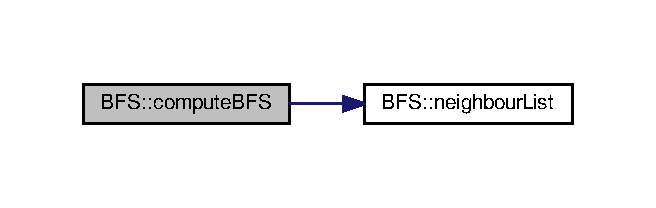
\includegraphics[width=315pt]{classBFS_a569f5936b7d708e928f6477548ffcdd2_cgraph}
\end{center}
\end{figure}


\index{B\+FS@{B\+FS}!get\+Distance@{get\+Distance}}
\index{get\+Distance@{get\+Distance}!B\+FS@{B\+FS}}
\subsubsection[{\texorpdfstring{get\+Distance(int, int)}{getDistance(int, int)}}]{\setlength{\rightskip}{0pt plus 5cm}int B\+F\+S\+::get\+Distance (
\begin{DoxyParamCaption}
\item[{int}]{x, }
\item[{int}]{y}
\end{DoxyParamCaption}
)}\hypertarget{classBFS_a59c2fa43dd3f00bc0524d264338da1d5}{}\label{classBFS_a59c2fa43dd3f00bc0524d264338da1d5}


function to get the distance value of a specific grid 


\begin{DoxyParams}{Parameters}
{\em x} & x-\/position of the grid \\
\hline
{\em y} & y-\/position of the grid\\
\hline
\end{DoxyParams}
\begin{DoxyReturn}{Returns}
integer value of distance grid for the x and y coordinates 
\end{DoxyReturn}


Definition at line 71 of file B\+F\+S.\+cpp.



References distance.



Referenced by T\+E\+S\+T().

\index{B\+FS@{B\+FS}!get\+Explored@{get\+Explored}}
\index{get\+Explored@{get\+Explored}!B\+FS@{B\+FS}}
\subsubsection[{\texorpdfstring{get\+Explored(int, int)}{getExplored(int, int)}}]{\setlength{\rightskip}{0pt plus 5cm}int B\+F\+S\+::get\+Explored (
\begin{DoxyParamCaption}
\item[{int}]{x, }
\item[{int}]{y}
\end{DoxyParamCaption}
)}\hypertarget{classBFS_af170bc63c82b8e814df7fd6a035303cc}{}\label{classBFS_af170bc63c82b8e814df7fd6a035303cc}


function to get the explored value of a specific grid 


\begin{DoxyParams}{Parameters}
{\em x} & x-\/position of the grid \\
\hline
{\em y} & y-\/position of the grid\\
\hline
\end{DoxyParams}
\begin{DoxyReturn}{Returns}
integer value of explored grid for the x and y coordinates 
\end{DoxyReturn}


Definition at line 66 of file B\+F\+S.\+cpp.



References explored.



Referenced by T\+E\+S\+T().

\index{B\+FS@{B\+FS}!neighbour\+List@{neighbour\+List}}
\index{neighbour\+List@{neighbour\+List}!B\+FS@{B\+FS}}
\subsubsection[{\texorpdfstring{neighbour\+List(const std\+::vector$<$ std\+::vector$<$ int $>$ $>$ \&, std\+::vector$<$ int $>$, std\+::queue$<$ std\+::vector$<$ int $>$ $>$ \&)}{neighbourList(const std::vector< std::vector< int > > &, std::vector< int >, std::queue< std::vector< int > > &)}}]{\setlength{\rightskip}{0pt plus 5cm}void B\+F\+S\+::neighbour\+List (
\begin{DoxyParamCaption}
\item[{const std\+::vector$<$ std\+::vector$<$ int $>$ $>$ \&}]{, }
\item[{std\+::vector$<$ int $>$}]{, }
\item[{std\+::queue$<$ std\+::vector$<$ int $>$ $>$ \&}]{}
\end{DoxyParamCaption}
)}\hypertarget{classBFS_a099fc340466239bed3cb23bcf3c6eeae}{}\label{classBFS_a099fc340466239bed3cb23bcf3c6eeae}


function to estimate the neighbouring node 


\begin{DoxyParams}{Parameters}
{\em frontier} & vector \\
\hline
{\em vector} & coordinate to which neighbouring node has to found out \\
\hline
{\em list} & of all neighbouring node of the given coordinate\\
\hline
\end{DoxyParams}
\begin{DoxyReturn}{Returns}
frontiers Queue to store all the frontiers 
\end{DoxyReturn}


Definition at line 76 of file B\+F\+S.\+cpp.



Referenced by compute\+B\+F\+S(), and T\+E\+S\+T().



\subsection{Member Data Documentation}
\index{B\+FS@{B\+FS}!distance@{distance}}
\index{distance@{distance}!B\+FS@{B\+FS}}
\subsubsection[{\texorpdfstring{distance}{distance}}]{\setlength{\rightskip}{0pt plus 5cm}std\+::vector$<$std\+::vector$<$int$>$ $>$ B\+F\+S\+::distance\hspace{0.3cm}{\ttfamily [private]}}\hypertarget{classBFS_afe579e465bd78cca7566530b0e006df2}{}\label{classBFS_afe579e465bd78cca7566530b0e006df2}


Definition at line 57 of file B\+F\+S.\+hpp.



Referenced by B\+F\+S(), compute\+B\+F\+S(), and get\+Distance().

\index{B\+FS@{B\+FS}!explored@{explored}}
\index{explored@{explored}!B\+FS@{B\+FS}}
\subsubsection[{\texorpdfstring{explored}{explored}}]{\setlength{\rightskip}{0pt plus 5cm}std\+::vector$<$std\+::vector$<$int$>$ $>$ B\+F\+S\+::explored\hspace{0.3cm}{\ttfamily [private]}}\hypertarget{classBFS_a2e5bcb2d5e51e544bbd5de47a470186d}{}\label{classBFS_a2e5bcb2d5e51e544bbd5de47a470186d}


Definition at line 59 of file B\+F\+S.\+hpp.



Referenced by B\+F\+S(), compute\+B\+F\+S(), and get\+Explored().

\index{B\+FS@{B\+FS}!p\+Queue@{p\+Queue}}
\index{p\+Queue@{p\+Queue}!B\+FS@{B\+FS}}
\subsubsection[{\texorpdfstring{p\+Queue}{pQueue}}]{\setlength{\rightskip}{0pt plus 5cm}std\+::queue$<$std\+::vector$<$int$>$ $>$ B\+F\+S\+::p\+Queue\hspace{0.3cm}{\ttfamily [private]}}\hypertarget{classBFS_a408e3b926379694275b0a1c967c12839}{}\label{classBFS_a408e3b926379694275b0a1c967c12839}


Definition at line 55 of file B\+F\+S.\+hpp.



Referenced by compute\+B\+F\+S().



The documentation for this class was generated from the following files\+:\begin{DoxyCompactItemize}
\item 
include/\hyperlink{BFS_8hpp}{B\+F\+S.\+hpp}\item 
src/\hyperlink{BFS_8cpp}{B\+F\+S.\+cpp}\end{DoxyCompactItemize}

\hypertarget{classexplore}{}\section{explore Class Reference}
\label{classexplore}\index{explore@{explore}}


Class to implement the \hyperlink{classBFS}{B\+FS}.  




{\ttfamily \#include $<$explore.\+hpp$>$}

\subsection*{Public Member Functions}
\begin{DoxyCompactItemize}
\item 
\hyperlink{classexplore_a1f0ce75d7c2beafbcd80320379788e7d}{explore} ()
\begin{DoxyCompactList}\small\item\em class constructor \end{DoxyCompactList}\item 
void \hyperlink{classexplore_a1e21ba2b5ae23bed33de7856e1418b64}{path\+Search} (std\+::vector$<$ int $>$, std\+::vector$<$ int $>$, \hyperlink{classmap}{map} \&)
\begin{DoxyCompactList}\small\item\em path\+Search to find the path to the goal \end{DoxyCompactList}\item 
bool \hyperlink{classexplore_a402fe39518e7024b1f49cd000c1620ed}{compute\+Shortest\+Path} (std\+::vector$<$ int $>$, std\+::vector$<$ int $>$, std\+::vector$<$ std\+::vector$<$ int $>$ $>$ \&, \hyperlink{classmap}{map} \&)
\begin{DoxyCompactList}\small\item\em function to compute the shortest path using \hyperlink{classBFS}{B\+FS} \end{DoxyCompactList}\item 
void \hyperlink{classexplore_ab529fa2c030a29a5ac687b26b61b0663}{find\+Obstacle\+Free\+Neighbours} (std\+::vector$<$ int $>$, std\+::queue$<$ std\+::vector$<$ int $>$ $>$ \&, \hyperlink{classmap}{map} \&)
\begin{DoxyCompactList}\small\item\em function to find the neighbour of the given point which is without the obstacle \end{DoxyCompactList}\item 
bool \hyperlink{classexplore_a668d5b972220ff43b4680beb1e889dd4}{navigate} (float, \hyperlink{classmap}{map} \&, std\+::vector$<$ int $>$)
\begin{DoxyCompactList}\small\item\em function to publish goal to the move base topic \end{DoxyCompactList}\item 
\hyperlink{classexplore_a65b7817d6755089698fa978f9e273750}{$\sim$explore} ()
\begin{DoxyCompactList}\small\item\em class destructor \end{DoxyCompactList}\end{DoxyCompactItemize}
\subsection*{Private Attributes}
\begin{DoxyCompactItemize}
\item 
std\+::vector$<$ std\+::vector$<$ int $>$ $>$ \hyperlink{classexplore_a3cb0f00e270d2da0bf7a3c1335f03cc4}{path}
\end{DoxyCompactItemize}


\subsection{Detailed Description}
Class to implement the \hyperlink{classBFS}{B\+FS}. 


\begin{DoxyParams}{Parameters}
{\em path} & vector to store the path\\
\hline
\end{DoxyParams}
\begin{DoxyReturn}{Returns}
None 
\end{DoxyReturn}


Definition at line 54 of file explore.\+hpp.



\subsection{Constructor \& Destructor Documentation}
\index{explore@{explore}!explore@{explore}}
\index{explore@{explore}!explore@{explore}}
\subsubsection[{\texorpdfstring{explore()}{explore()}}]{\setlength{\rightskip}{0pt plus 5cm}explore\+::explore (
\begin{DoxyParamCaption}
{}
\end{DoxyParamCaption}
)}\hypertarget{classexplore_a1f0ce75d7c2beafbcd80320379788e7d}{}\label{classexplore_a1f0ce75d7c2beafbcd80320379788e7d}


class constructor 

\begin{DoxyReturn}{Returns}
None 
\end{DoxyReturn}


Definition at line 51 of file explore.\+cpp.

\index{explore@{explore}!````~explore@{$\sim$explore}}
\index{````~explore@{$\sim$explore}!explore@{explore}}
\subsubsection[{\texorpdfstring{$\sim$explore()}{~explore()}}]{\setlength{\rightskip}{0pt plus 5cm}explore\+::$\sim$explore (
\begin{DoxyParamCaption}
{}
\end{DoxyParamCaption}
)}\hypertarget{classexplore_a65b7817d6755089698fa978f9e273750}{}\label{classexplore_a65b7817d6755089698fa978f9e273750}


class destructor 

\begin{DoxyReturn}{Returns}
None 
\end{DoxyReturn}


Definition at line 250 of file explore.\+cpp.



\subsection{Member Function Documentation}
\index{explore@{explore}!compute\+Shortest\+Path@{compute\+Shortest\+Path}}
\index{compute\+Shortest\+Path@{compute\+Shortest\+Path}!explore@{explore}}
\subsubsection[{\texorpdfstring{compute\+Shortest\+Path(std\+::vector$<$ int $>$, std\+::vector$<$ int $>$, std\+::vector$<$ std\+::vector$<$ int $>$ $>$ \&, map \&)}{computeShortestPath(std::vector< int >, std::vector< int >, std::vector< std::vector< int > > &, map &)}}]{\setlength{\rightskip}{0pt plus 5cm}bool explore\+::compute\+Shortest\+Path (
\begin{DoxyParamCaption}
\item[{std\+::vector$<$ int $>$}]{start, }
\item[{std\+::vector$<$ int $>$}]{End, }
\item[{std\+::vector$<$ std\+::vector$<$ int $>$ $>$ \&}]{path1, }
\item[{{\bf map} \&}]{obj}
\end{DoxyParamCaption}
)}\hypertarget{classexplore_a402fe39518e7024b1f49cd000c1620ed}{}\label{classexplore_a402fe39518e7024b1f49cd000c1620ed}


function to compute the shortest path using \hyperlink{classBFS}{B\+FS} 


\begin{DoxyParams}{Parameters}
{\em start} & vector contains the start point for the path \\
\hline
{\em end} & vector contains the end point for the path \\
\hline
{\em path} & that stores the path to the goal \\
\hline
{\em map} & Object to get the rows, grid value and column\\
\hline
\end{DoxyParams}
\begin{DoxyReturn}{Returns}
bool 
\end{DoxyReturn}


Definition at line 83 of file explore.\+cpp.



References find\+Obstacle\+Free\+Neighbours(), path, map\+::return\+Cols(), and map\+::return\+Rows().



Referenced by path\+Search(), and T\+E\+S\+T().



Here is the call graph for this function\+:
\nopagebreak
\begin{figure}[H]
\begin{center}
\leavevmode
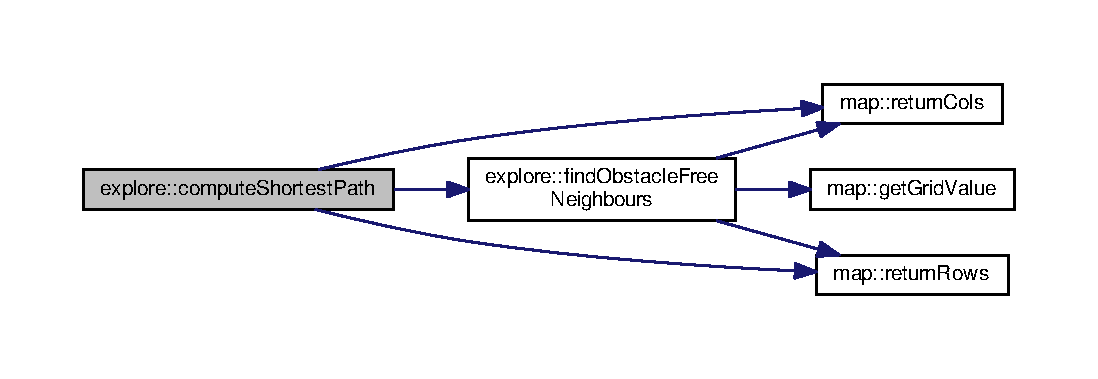
\includegraphics[width=350pt]{classexplore_a402fe39518e7024b1f49cd000c1620ed_cgraph}
\end{center}
\end{figure}


\index{explore@{explore}!find\+Obstacle\+Free\+Neighbours@{find\+Obstacle\+Free\+Neighbours}}
\index{find\+Obstacle\+Free\+Neighbours@{find\+Obstacle\+Free\+Neighbours}!explore@{explore}}
\subsubsection[{\texorpdfstring{find\+Obstacle\+Free\+Neighbours(std\+::vector$<$ int $>$, std\+::queue$<$ std\+::vector$<$ int $>$ $>$ \&, map \&)}{findObstacleFreeNeighbours(std::vector< int >, std::queue< std::vector< int > > &, map &)}}]{\setlength{\rightskip}{0pt plus 5cm}void explore\+::find\+Obstacle\+Free\+Neighbours (
\begin{DoxyParamCaption}
\item[{std\+::vector$<$ int $>$}]{v, }
\item[{std\+::queue$<$ std\+::vector$<$ int $>$ $>$ \&}]{list, }
\item[{{\bf map} \&}]{obj}
\end{DoxyParamCaption}
)}\hypertarget{classexplore_ab529fa2c030a29a5ac687b26b61b0663}{}\label{classexplore_ab529fa2c030a29a5ac687b26b61b0663}


function to find the neighbour of the given point which is without the obstacle 


\begin{DoxyParams}{Parameters}
{\em v} & vector contains the point to which neighbour has to be found \\
\hline
{\em list} & is a queue contains the list of neighbour \\
\hline
{\em map} & Object to get rows and columns\\
\hline
\end{DoxyParams}
\begin{DoxyReturn}{Returns}
None 
\end{DoxyReturn}


Definition at line 54 of file explore.\+cpp.



References map\+::get\+Grid\+Value(), map\+::return\+Cols(), and map\+::return\+Rows().



Referenced by compute\+Shortest\+Path(), and T\+E\+S\+T().



Here is the call graph for this function\+:
\nopagebreak
\begin{figure}[H]
\begin{center}
\leavevmode
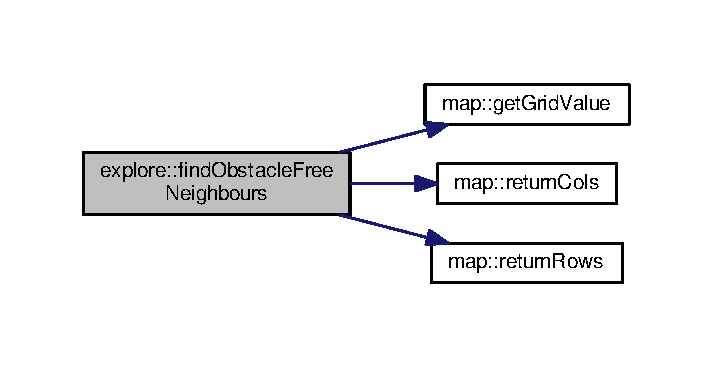
\includegraphics[width=342pt]{classexplore_ab529fa2c030a29a5ac687b26b61b0663_cgraph}
\end{center}
\end{figure}


\index{explore@{explore}!navigate@{navigate}}
\index{navigate@{navigate}!explore@{explore}}
\subsubsection[{\texorpdfstring{navigate(float, map \&, std\+::vector$<$ int $>$)}{navigate(float, map &, std::vector< int >)}}]{\setlength{\rightskip}{0pt plus 5cm}bool explore\+::navigate (
\begin{DoxyParamCaption}
\item[{float}]{resolution, }
\item[{{\bf map} \&}]{obj, }
\item[{std\+::vector$<$ int $>$}]{pos}
\end{DoxyParamCaption}
)}\hypertarget{classexplore_a668d5b972220ff43b4680beb1e889dd4}{}\label{classexplore_a668d5b972220ff43b4680beb1e889dd4}


function to publish goal to the move base topic 


\begin{DoxyParams}{Parameters}
{\em resolution} & is a float that contains the resolution of the map \\
\hline
{\em map} & Object to get the rows, column\\
\hline
\end{DoxyParams}
\begin{DoxyReturn}{Returns}
bool whether it has reached the target or not 
\end{DoxyReturn}


Definition at line 165 of file explore.\+cpp.



References path, map\+::return\+Cols(), and map\+::return\+Rows().



Referenced by main().



Here is the call graph for this function\+:
\nopagebreak
\begin{figure}[H]
\begin{center}
\leavevmode
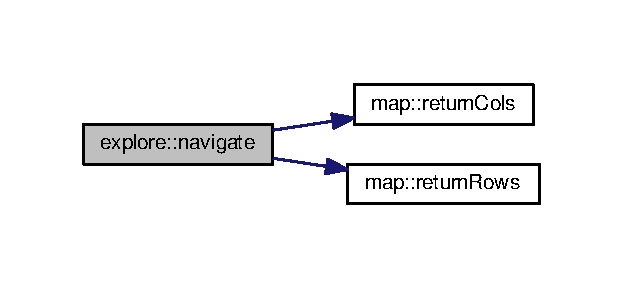
\includegraphics[width=299pt]{classexplore_a668d5b972220ff43b4680beb1e889dd4_cgraph}
\end{center}
\end{figure}


\index{explore@{explore}!path\+Search@{path\+Search}}
\index{path\+Search@{path\+Search}!explore@{explore}}
\subsubsection[{\texorpdfstring{path\+Search(std\+::vector$<$ int $>$, std\+::vector$<$ int $>$, map \&)}{pathSearch(std::vector< int >, std::vector< int >, map &)}}]{\setlength{\rightskip}{0pt plus 5cm}void explore\+::path\+Search (
\begin{DoxyParamCaption}
\item[{std\+::vector$<$ int $>$}]{start, }
\item[{std\+::vector$<$ int $>$}]{end, }
\item[{{\bf map} \&}]{obj}
\end{DoxyParamCaption}
)}\hypertarget{classexplore_a1e21ba2b5ae23bed33de7856e1418b64}{}\label{classexplore_a1e21ba2b5ae23bed33de7856e1418b64}


path\+Search to find the path to the goal 


\begin{DoxyParams}{Parameters}
{\em start} & contains the start point for the path \\
\hline
{\em end} & contains the end point for the path \\
\hline
{\em map} & object to get rows and columns\\
\hline
\end{DoxyParams}
\begin{DoxyReturn}{Returns}
None 
\end{DoxyReturn}


Definition at line 155 of file explore.\+cpp.



References compute\+Shortest\+Path(), and path.



Referenced by main().



Here is the call graph for this function\+:
\nopagebreak
\begin{figure}[H]
\begin{center}
\leavevmode
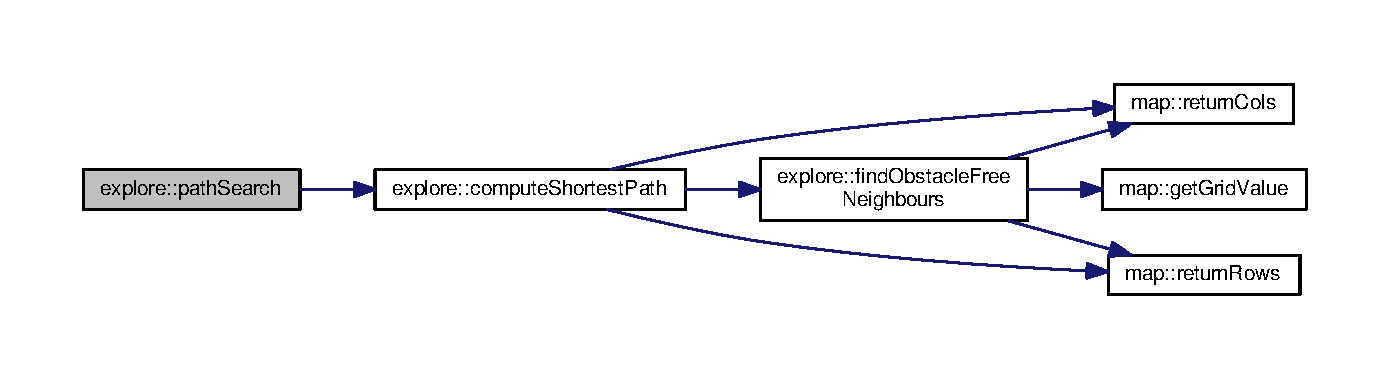
\includegraphics[width=350pt]{classexplore_a1e21ba2b5ae23bed33de7856e1418b64_cgraph}
\end{center}
\end{figure}




\subsection{Member Data Documentation}
\index{explore@{explore}!path@{path}}
\index{path@{path}!explore@{explore}}
\subsubsection[{\texorpdfstring{path}{path}}]{\setlength{\rightskip}{0pt plus 5cm}std\+::vector$<$std\+::vector$<$int$>$ $>$ explore\+::path\hspace{0.3cm}{\ttfamily [private]}}\hypertarget{classexplore_a3cb0f00e270d2da0bf7a3c1335f03cc4}{}\label{classexplore_a3cb0f00e270d2da0bf7a3c1335f03cc4}


Definition at line 57 of file explore.\+hpp.



Referenced by compute\+Shortest\+Path(), navigate(), and path\+Search().



The documentation for this class was generated from the following files\+:\begin{DoxyCompactItemize}
\item 
include/\hyperlink{explore_8hpp}{explore.\+hpp}\item 
src/\hyperlink{explore_8cpp}{explore.\+cpp}\end{DoxyCompactItemize}

\hypertarget{classmap}{}\section{map Class Reference}
\label{classmap}\index{map@{map}}


Class to implement the M\+AP.  




{\ttfamily \#include $<$map.\+hpp$>$}

\subsection*{Public Member Functions}
\begin{DoxyCompactItemize}
\item 
\hyperlink{classmap_abedfe6722ad83929739afd899c88fea4}{map} ()
\begin{DoxyCompactList}\small\item\em Constructor for the class map. \end{DoxyCompactList}\item 
void \hyperlink{classmap_acaa7a0726870c1d08c75b3f84caa298b}{frontier\+Search} (int, int)
\begin{DoxyCompactList}\small\item\em Function to search frontiers in the map. \end{DoxyCompactList}\item 
bool \hyperlink{classmap_a5e55d5c21318b0036147b9ea558c6983}{check\+Neighbour} (int, int, int)
\begin{DoxyCompactList}\small\item\em Function to check if the neighbour\textquotesingle{}s grid value. \end{DoxyCompactList}\item 
std\+::vector$<$ int $>$ \hyperlink{classmap_ad07d469282f85b48d181e530a886b335}{compute\+Frontier\+Centroid} (const std\+::queue$<$ std\+::vector$<$ int $>$$>$ \&)
\begin{DoxyCompactList}\small\item\em Function to compute the centroid of the frontier. \end{DoxyCompactList}\item 
std\+::vector$<$ int $>$ \hyperlink{classmap_a300d8aaac77b805595e640205aad1cb0}{nearest} (const std\+::queue$<$ std\+::vector$<$ int $>$$>$ \&, int, int)
\begin{DoxyCompactList}\small\item\em Function to find the point closest to computed centroid. \end{DoxyCompactList}\item 
bool \hyperlink{classmap_ad0c8afa9f68ede5257f5b7b2d33b093f}{request\+Map} (ros\+::\+Node\+Handle \&)
\begin{DoxyCompactList}\small\item\em Function to request map from gmapping node. \end{DoxyCompactList}\item 
void \hyperlink{classmap_ad3a6b0b96fc74179816e7a4ed785fc4d}{mapcallback} (const nav\+\_\+msgs\+::\+Occupancy\+Grid \&msg)
\begin{DoxyCompactList}\small\item\em Call\+Back function for the map subscriber. \end{DoxyCompactList}\item 
std\+::vector$<$ int $>$ \hyperlink{classmap_a69743a83eb45ec5cef3fbc07aae26427}{nearest\+Centroid} (int, int)
\begin{DoxyCompactList}\small\item\em Function to find the point closest to computed centroid. \end{DoxyCompactList}\item 
int \hyperlink{classmap_a696bcdd2197355d1ff65e6fdf90cad46}{get\+Grid\+Value} (int, int)
\begin{DoxyCompactList}\small\item\em Function to return the grid value. \end{DoxyCompactList}\item 
int \hyperlink{classmap_af9092b505e0d7f793322c7a481e3ca88}{get\+Centroid\+Size} ()
\begin{DoxyCompactList}\small\item\em Function to return the size of centroid queue. \end{DoxyCompactList}\item 
int \hyperlink{classmap_a665740b6cec1d2fac63bf1a9985e9628}{return\+Rows} ()
\begin{DoxyCompactList}\small\item\em Function to return row size. \end{DoxyCompactList}\item 
int \hyperlink{classmap_abffb3a9e6f9e18a73695b62e42d0811c}{return\+Cols} ()
\begin{DoxyCompactList}\small\item\em Function to return coloumn size. \end{DoxyCompactList}\item 
float \hyperlink{classmap_abd2282cb63fd166dbf2e90f78f610953}{get\+Resolution} ()
\begin{DoxyCompactList}\small\item\em Function to return resolution of the map. \end{DoxyCompactList}\item 
std\+::vector$<$ int $>$ \hyperlink{classmap_a51047b6cd09491df72de1447c7c99431}{get\+Start} ()
\begin{DoxyCompactList}\small\item\em Function to return origin. \end{DoxyCompactList}\item 
\hyperlink{classmap_a0cc22df7b44f7835fa10ed241848b041}{$\sim$map} ()
\begin{DoxyCompactList}\small\item\em Destructor for the class map. \end{DoxyCompactList}\end{DoxyCompactItemize}
\subsection*{Public Attributes}
\begin{DoxyCompactItemize}
\item 
std\+::vector$<$ int $>$ \hyperlink{classmap_a73ea3c7b79de5a8b5733b7babc21e68b}{start}
\end{DoxyCompactItemize}
\subsection*{Private Attributes}
\begin{DoxyCompactItemize}
\item 
std\+::queue$<$ std\+::vector$<$ int $>$ $>$ \hyperlink{classmap_ad3683241c11549fa2888eadf3465857f}{frontier\+Queue}
\item 
std\+::queue$<$ std\+::vector$<$ int $>$ $>$ \hyperlink{classmap_a8fe868100933bfd68b502b68d42f1883}{centroid\+Queue}
\item 
std\+::queue$<$ std\+::vector$<$ int $>$ $>$ \hyperlink{classmap_ad8a2f40c1520dd9f0f5337abbf81e64f}{explored}
\item 
std\+::vector$<$ std\+::vector$<$ int $>$ $>$ \hyperlink{classmap_a43036b0bcee6beeb4e8f4dfc5019e5fb}{grid}
\item 
int \hyperlink{classmap_a2ee828fe96a115fe070e8ff8eea7b488}{rows}
\item 
int \hyperlink{classmap_ad82f9850ab232d78d0cac14c5e6a752f}{cols}
\item 
float \hyperlink{classmap_ab2c38de30b06b80ec0a6ce646056d33a}{map\+Resolution}
\item 
ros\+::\+Subscriber \hyperlink{classmap_ae40cfd9b303640dfc7a56e198056d2a0}{O\+G\+M\+\_\+subscriber}
\end{DoxyCompactItemize}


\subsection{Detailed Description}
Class to implement the M\+AP. 


\begin{DoxyParams}{Parameters}
{\em frontier} & queue to hold the frontier points \\
\hline
{\em Centroid} & queue to hold the centroid of individual frontiers \\
\hline
{\em grid} & the map as 2d vector \\
\hline
{\em row} & integer with row size of grid \\
\hline
{\em cols} & integer with coloumn size of grid \\
\hline
{\em map\+Resolution} & integer with resolution of grid \\
\hline
{\em O\+G\+M\+\_\+\+Subscriber} & is the subscriber handle for /\+Map \\
\hline
{\em start} & vector containing the origin \\
\hline
\end{DoxyParams}
\begin{DoxyReturn}{Returns}
none 
\end{DoxyReturn}


Definition at line 63 of file map.\+hpp.



\subsection{Constructor \& Destructor Documentation}
\index{map@{map}!map@{map}}
\index{map@{map}!map@{map}}
\subsubsection[{\texorpdfstring{map()}{map()}}]{\setlength{\rightskip}{0pt plus 5cm}map\+::map (
\begin{DoxyParamCaption}
{}
\end{DoxyParamCaption}
)}\hypertarget{classmap_abedfe6722ad83929739afd899c88fea4}{}\label{classmap_abedfe6722ad83929739afd899c88fea4}


Constructor for the class map. 


\begin{DoxyParams}{Parameters}
{\em None} & \\
\hline
\end{DoxyParams}
\begin{DoxyReturn}{Returns}
None 
\end{DoxyReturn}


Definition at line 51 of file map.\+cpp.



References cols, grid, map\+Resolution, and rows.



Referenced by frontier\+Search().

\index{map@{map}!````~map@{$\sim$map}}
\index{````~map@{$\sim$map}!map@{map}}
\subsubsection[{\texorpdfstring{$\sim$map()}{~map()}}]{\setlength{\rightskip}{0pt plus 5cm}map\+::$\sim$map (
\begin{DoxyParamCaption}
{}
\end{DoxyParamCaption}
)}\hypertarget{classmap_a0cc22df7b44f7835fa10ed241848b041}{}\label{classmap_a0cc22df7b44f7835fa10ed241848b041}


Destructor for the class map. 


\begin{DoxyParams}{Parameters}
{\em None} & \\
\hline
\end{DoxyParams}
\begin{DoxyReturn}{Returns}
None 
\end{DoxyReturn}


Definition at line 284 of file map.\+cpp.



\subsection{Member Function Documentation}
\index{map@{map}!check\+Neighbour@{check\+Neighbour}}
\index{check\+Neighbour@{check\+Neighbour}!map@{map}}
\subsubsection[{\texorpdfstring{check\+Neighbour(int, int, int)}{checkNeighbour(int, int, int)}}]{\setlength{\rightskip}{0pt plus 5cm}bool map\+::check\+Neighbour (
\begin{DoxyParamCaption}
\item[{int}]{x\+Point, }
\item[{int}]{y\+Point, }
\item[{int}]{mode}
\end{DoxyParamCaption}
)}\hypertarget{classmap_a5e55d5c21318b0036147b9ea558c6983}{}\label{classmap_a5e55d5c21318b0036147b9ea558c6983}


Function to check if the neighbour\textquotesingle{}s grid value. 


\begin{DoxyParams}{Parameters}
{\em X} & coordinate of grid \\
\hline
{\em Y} & coordinate of grid \\
\hline
{\em Value} & to be checked \\
\hline
\end{DoxyParams}
\begin{DoxyReturn}{Returns}
Check 
\end{DoxyReturn}


Definition at line 124 of file map.\+cpp.



References grid.



Referenced by frontier\+Search(), and T\+E\+S\+T().

\index{map@{map}!compute\+Frontier\+Centroid@{compute\+Frontier\+Centroid}}
\index{compute\+Frontier\+Centroid@{compute\+Frontier\+Centroid}!map@{map}}
\subsubsection[{\texorpdfstring{compute\+Frontier\+Centroid(const std\+::queue$<$ std\+::vector$<$ int $>$$>$ \&)}{computeFrontierCentroid(const std::queue< std::vector< int >> &)}}]{\setlength{\rightskip}{0pt plus 5cm}std\+::vector$<$ int $>$ map\+::compute\+Frontier\+Centroid (
\begin{DoxyParamCaption}
\item[{const std\+::queue$<$ std\+::vector$<$ int $>$$>$ \&}]{q}
\end{DoxyParamCaption}
)}\hypertarget{classmap_ad07d469282f85b48d181e530a886b335}{}\label{classmap_ad07d469282f85b48d181e530a886b335}


Function to compute the centroid of the frontier. 


\begin{DoxyParams}{Parameters}
{\em Frontier} & Queue containing the centroid coordinates \\
\hline
\end{DoxyParams}
\begin{DoxyReturn}{Returns}
Centroid point 
\end{DoxyReturn}


Definition at line 173 of file map.\+cpp.



References nearest().



Referenced by frontier\+Search(), and T\+E\+S\+T().



Here is the call graph for this function\+:
\nopagebreak
\begin{figure}[H]
\begin{center}
\leavevmode
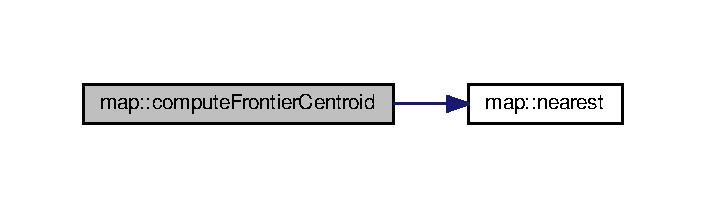
\includegraphics[width=339pt]{classmap_ad07d469282f85b48d181e530a886b335_cgraph}
\end{center}
\end{figure}


\index{map@{map}!frontier\+Search@{frontier\+Search}}
\index{frontier\+Search@{frontier\+Search}!map@{map}}
\subsubsection[{\texorpdfstring{frontier\+Search(int, int)}{frontierSearch(int, int)}}]{\setlength{\rightskip}{0pt plus 5cm}void map\+::frontier\+Search (
\begin{DoxyParamCaption}
\item[{int}]{height, }
\item[{int}]{width}
\end{DoxyParamCaption}
)}\hypertarget{classmap_acaa7a0726870c1d08c75b3f84caa298b}{}\label{classmap_acaa7a0726870c1d08c75b3f84caa298b}


Function to search frontiers in the map. 


\begin{DoxyParams}{Parameters}
{\em X} & coordinate of grid \\
\hline
{\em Y} & coordinate of grid \\
\hline
\end{DoxyParams}
\begin{DoxyReturn}{Returns}
none 
\end{DoxyReturn}


Definition at line 195 of file map.\+cpp.



References centroid\+Queue, check\+Neighbour(), B\+F\+S\+::compute\+B\+F\+S(), compute\+Frontier\+Centroid(), explored, frontier\+Queue, grid, and map().



Referenced by main(), and T\+E\+S\+T().



Here is the call graph for this function\+:
\nopagebreak
\begin{figure}[H]
\begin{center}
\leavevmode
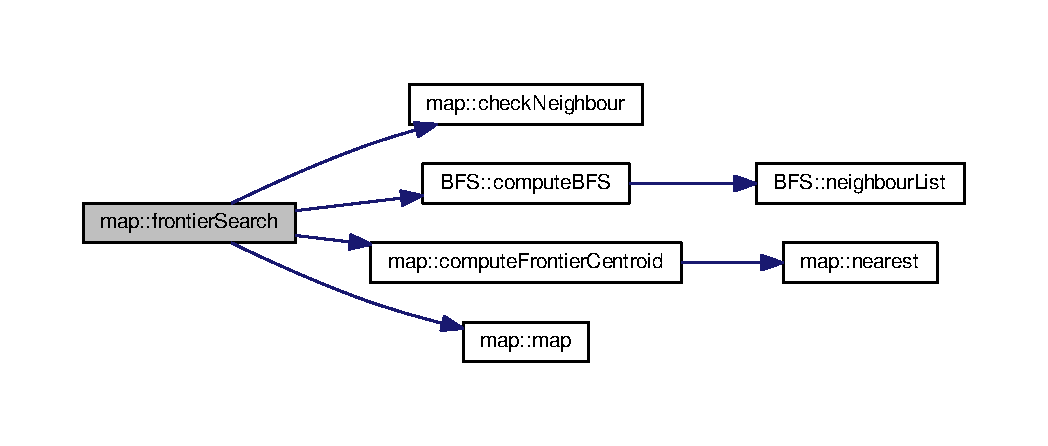
\includegraphics[width=350pt]{classmap_acaa7a0726870c1d08c75b3f84caa298b_cgraph}
\end{center}
\end{figure}


\index{map@{map}!get\+Centroid\+Size@{get\+Centroid\+Size}}
\index{get\+Centroid\+Size@{get\+Centroid\+Size}!map@{map}}
\subsubsection[{\texorpdfstring{get\+Centroid\+Size()}{getCentroidSize()}}]{\setlength{\rightskip}{0pt plus 5cm}int map\+::get\+Centroid\+Size (
\begin{DoxyParamCaption}
{}
\end{DoxyParamCaption}
)}\hypertarget{classmap_af9092b505e0d7f793322c7a481e3ca88}{}\label{classmap_af9092b505e0d7f793322c7a481e3ca88}


Function to return the size of centroid queue. 


\begin{DoxyParams}{Parameters}
{\em None} & \\
\hline
\end{DoxyParams}
\begin{DoxyReturn}{Returns}
centroid size 
\end{DoxyReturn}


Definition at line 120 of file map.\+cpp.



References centroid\+Queue.



Referenced by T\+E\+S\+T().

\index{map@{map}!get\+Grid\+Value@{get\+Grid\+Value}}
\index{get\+Grid\+Value@{get\+Grid\+Value}!map@{map}}
\subsubsection[{\texorpdfstring{get\+Grid\+Value(int, int)}{getGridValue(int, int)}}]{\setlength{\rightskip}{0pt plus 5cm}int map\+::get\+Grid\+Value (
\begin{DoxyParamCaption}
\item[{int}]{x, }
\item[{int}]{y}
\end{DoxyParamCaption}
)}\hypertarget{classmap_a696bcdd2197355d1ff65e6fdf90cad46}{}\label{classmap_a696bcdd2197355d1ff65e6fdf90cad46}


Function to return the grid value. 


\begin{DoxyParams}{Parameters}
{\em X} & coordinate \\
\hline
{\em Y} & coordinate \\
\hline
\end{DoxyParams}
\begin{DoxyReturn}{Returns}
Grid value 
\end{DoxyReturn}


Definition at line 108 of file map.\+cpp.



References grid.



Referenced by explore\+::find\+Obstacle\+Free\+Neighbours(), and T\+E\+S\+T().

\index{map@{map}!get\+Resolution@{get\+Resolution}}
\index{get\+Resolution@{get\+Resolution}!map@{map}}
\subsubsection[{\texorpdfstring{get\+Resolution()}{getResolution()}}]{\setlength{\rightskip}{0pt plus 5cm}float map\+::get\+Resolution (
\begin{DoxyParamCaption}
{}
\end{DoxyParamCaption}
)}\hypertarget{classmap_abd2282cb63fd166dbf2e90f78f610953}{}\label{classmap_abd2282cb63fd166dbf2e90f78f610953}


Function to return resolution of the map. 


\begin{DoxyParams}{Parameters}
{\em None} & \\
\hline
\end{DoxyParams}
\begin{DoxyReturn}{Returns}
resolution of the map 
\end{DoxyReturn}


Definition at line 280 of file map.\+cpp.



References map\+Resolution.



Referenced by main(), and T\+E\+S\+T().

\index{map@{map}!get\+Start@{get\+Start}}
\index{get\+Start@{get\+Start}!map@{map}}
\subsubsection[{\texorpdfstring{get\+Start()}{getStart()}}]{\setlength{\rightskip}{0pt plus 5cm}std\+::vector$<$ int $>$ map\+::get\+Start (
\begin{DoxyParamCaption}
{}
\end{DoxyParamCaption}
)}\hypertarget{classmap_a51047b6cd09491df72de1447c7c99431}{}\label{classmap_a51047b6cd09491df72de1447c7c99431}


Function to return origin. 


\begin{DoxyParams}{Parameters}
{\em None} & \\
\hline
\end{DoxyParams}
\begin{DoxyReturn}{Returns}
origin vector 
\end{DoxyReturn}


Definition at line 276 of file map.\+cpp.



References start.



Referenced by main().

\index{map@{map}!mapcallback@{mapcallback}}
\index{mapcallback@{mapcallback}!map@{map}}
\subsubsection[{\texorpdfstring{mapcallback(const nav\+\_\+msgs\+::\+Occupancy\+Grid \&msg)}{mapcallback(const nav_msgs::OccupancyGrid &msg)}}]{\setlength{\rightskip}{0pt plus 5cm}void map\+::mapcallback (
\begin{DoxyParamCaption}
\item[{const nav\+\_\+msgs\+::\+Occupancy\+Grid \&}]{msg}
\end{DoxyParamCaption}
)}\hypertarget{classmap_ad3a6b0b96fc74179816e7a4ed785fc4d}{}\label{classmap_ad3a6b0b96fc74179816e7a4ed785fc4d}


Call\+Back function for the map subscriber. 


\begin{DoxyParams}{Parameters}
{\em Contains} & the map in as occupancy grid in row major form \\
\hline
\end{DoxyParams}
\begin{DoxyReturn}{Returns}
none 
\end{DoxyReturn}


Definition at line 76 of file map.\+cpp.



References cols, grid, map\+Resolution, rows, and start.



Referenced by request\+Map().

\index{map@{map}!nearest@{nearest}}
\index{nearest@{nearest}!map@{map}}
\subsubsection[{\texorpdfstring{nearest(const std\+::queue$<$ std\+::vector$<$ int $>$$>$ \&, int, int)}{nearest(const std::queue< std::vector< int >> &, int, int)}}]{\setlength{\rightskip}{0pt plus 5cm}std\+::vector$<$ int $>$ map\+::nearest (
\begin{DoxyParamCaption}
\item[{const std\+::queue$<$ std\+::vector$<$ int $>$$>$ \&}]{q, }
\item[{int}]{centroidx, }
\item[{int}]{centroidy}
\end{DoxyParamCaption}
)}\hypertarget{classmap_a300d8aaac77b805595e640205aad1cb0}{}\label{classmap_a300d8aaac77b805595e640205aad1cb0}


Function to find the point closest to computed centroid. 


\begin{DoxyParams}{Parameters}
{\em Frontier} & Queue containing individual frontier points \\
\hline
\end{DoxyParams}
\begin{DoxyReturn}{Returns}
Point on frontier nearest to centroid 
\end{DoxyReturn}


Definition at line 148 of file map.\+cpp.



Referenced by compute\+Frontier\+Centroid(), and T\+E\+S\+T().

\index{map@{map}!nearest\+Centroid@{nearest\+Centroid}}
\index{nearest\+Centroid@{nearest\+Centroid}!map@{map}}
\subsubsection[{\texorpdfstring{nearest\+Centroid(int, int)}{nearestCentroid(int, int)}}]{\setlength{\rightskip}{0pt plus 5cm}std\+::vector$<$ int $>$ map\+::nearest\+Centroid (
\begin{DoxyParamCaption}
\item[{int}]{startX, }
\item[{int}]{startY}
\end{DoxyParamCaption}
)}\hypertarget{classmap_a69743a83eb45ec5cef3fbc07aae26427}{}\label{classmap_a69743a83eb45ec5cef3fbc07aae26427}


Function to find the point closest to computed centroid. 


\begin{DoxyParams}{Parameters}
{\em Frontier} & Queue containing individual frontier points \\
\hline
\end{DoxyParams}
\begin{DoxyReturn}{Returns}
Point on frontier nearest to centroid 
\end{DoxyReturn}


Definition at line 248 of file map.\+cpp.



References centroid\+Queue.



Referenced by main().

\index{map@{map}!request\+Map@{request\+Map}}
\index{request\+Map@{request\+Map}!map@{map}}
\subsubsection[{\texorpdfstring{request\+Map(ros\+::\+Node\+Handle \&)}{requestMap(ros::NodeHandle &)}}]{\setlength{\rightskip}{0pt plus 5cm}bool map\+::request\+Map (
\begin{DoxyParamCaption}
\item[{ros\+::\+Node\+Handle \&}]{nh}
\end{DoxyParamCaption}
)}\hypertarget{classmap_ad0c8afa9f68ede5257f5b7b2d33b093f}{}\label{classmap_ad0c8afa9f68ede5257f5b7b2d33b093f}


Function to request map from gmapping node. 


\begin{DoxyParams}{Parameters}
{\em Node} & handle \\
\hline
\end{DoxyParams}
\begin{DoxyReturn}{Returns}
Check if map is received 
\end{DoxyReturn}


Definition at line 70 of file map.\+cpp.



References mapcallback(), and O\+G\+M\+\_\+subscriber.



Referenced by main(), and T\+E\+S\+T().



Here is the call graph for this function\+:
\nopagebreak
\begin{figure}[H]
\begin{center}
\leavevmode
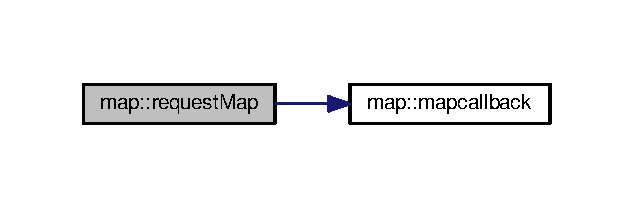
\includegraphics[width=304pt]{classmap_ad0c8afa9f68ede5257f5b7b2d33b093f_cgraph}
\end{center}
\end{figure}


\index{map@{map}!return\+Cols@{return\+Cols}}
\index{return\+Cols@{return\+Cols}!map@{map}}
\subsubsection[{\texorpdfstring{return\+Cols()}{returnCols()}}]{\setlength{\rightskip}{0pt plus 5cm}int map\+::return\+Cols (
\begin{DoxyParamCaption}
{}
\end{DoxyParamCaption}
)}\hypertarget{classmap_abffb3a9e6f9e18a73695b62e42d0811c}{}\label{classmap_abffb3a9e6f9e18a73695b62e42d0811c}


Function to return coloumn size. 


\begin{DoxyParams}{Parameters}
{\em None} & \\
\hline
\end{DoxyParams}
\begin{DoxyReturn}{Returns}
coloumn size 
\end{DoxyReturn}


Definition at line 116 of file map.\+cpp.



References cols.



Referenced by explore\+::compute\+Shortest\+Path(), explore\+::find\+Obstacle\+Free\+Neighbours(), main(), explore\+::navigate(), sensor\+::sensor(), and T\+E\+S\+T().

\index{map@{map}!return\+Rows@{return\+Rows}}
\index{return\+Rows@{return\+Rows}!map@{map}}
\subsubsection[{\texorpdfstring{return\+Rows()}{returnRows()}}]{\setlength{\rightskip}{0pt plus 5cm}int map\+::return\+Rows (
\begin{DoxyParamCaption}
{}
\end{DoxyParamCaption}
)}\hypertarget{classmap_a665740b6cec1d2fac63bf1a9985e9628}{}\label{classmap_a665740b6cec1d2fac63bf1a9985e9628}


Function to return row size. 


\begin{DoxyParams}{Parameters}
{\em None} & \\
\hline
\end{DoxyParams}
\begin{DoxyReturn}{Returns}
row size 
\end{DoxyReturn}


Definition at line 112 of file map.\+cpp.



References rows.



Referenced by explore\+::compute\+Shortest\+Path(), explore\+::find\+Obstacle\+Free\+Neighbours(), main(), explore\+::navigate(), sensor\+::sensor(), and T\+E\+S\+T().



\subsection{Member Data Documentation}
\index{map@{map}!centroid\+Queue@{centroid\+Queue}}
\index{centroid\+Queue@{centroid\+Queue}!map@{map}}
\subsubsection[{\texorpdfstring{centroid\+Queue}{centroidQueue}}]{\setlength{\rightskip}{0pt plus 5cm}std\+::queue$<$std\+::vector$<$int$>$ $>$ map\+::centroid\+Queue\hspace{0.3cm}{\ttfamily [private]}}\hypertarget{classmap_a8fe868100933bfd68b502b68d42f1883}{}\label{classmap_a8fe868100933bfd68b502b68d42f1883}


Definition at line 66 of file map.\+hpp.



Referenced by frontier\+Search(), get\+Centroid\+Size(), and nearest\+Centroid().

\index{map@{map}!cols@{cols}}
\index{cols@{cols}!map@{map}}
\subsubsection[{\texorpdfstring{cols}{cols}}]{\setlength{\rightskip}{0pt plus 5cm}int map\+::cols\hspace{0.3cm}{\ttfamily [private]}}\hypertarget{classmap_ad82f9850ab232d78d0cac14c5e6a752f}{}\label{classmap_ad82f9850ab232d78d0cac14c5e6a752f}


Definition at line 69 of file map.\+hpp.



Referenced by map(), mapcallback(), and return\+Cols().

\index{map@{map}!explored@{explored}}
\index{explored@{explored}!map@{map}}
\subsubsection[{\texorpdfstring{explored}{explored}}]{\setlength{\rightskip}{0pt plus 5cm}std\+::queue$<$std\+::vector$<$int$>$ $>$ map\+::explored\hspace{0.3cm}{\ttfamily [private]}}\hypertarget{classmap_ad8a2f40c1520dd9f0f5337abbf81e64f}{}\label{classmap_ad8a2f40c1520dd9f0f5337abbf81e64f}


Definition at line 67 of file map.\+hpp.



Referenced by frontier\+Search().

\index{map@{map}!frontier\+Queue@{frontier\+Queue}}
\index{frontier\+Queue@{frontier\+Queue}!map@{map}}
\subsubsection[{\texorpdfstring{frontier\+Queue}{frontierQueue}}]{\setlength{\rightskip}{0pt plus 5cm}std\+::queue$<$std\+::vector$<$int$>$ $>$ map\+::frontier\+Queue\hspace{0.3cm}{\ttfamily [private]}}\hypertarget{classmap_ad3683241c11549fa2888eadf3465857f}{}\label{classmap_ad3683241c11549fa2888eadf3465857f}


Definition at line 65 of file map.\+hpp.



Referenced by frontier\+Search().

\index{map@{map}!grid@{grid}}
\index{grid@{grid}!map@{map}}
\subsubsection[{\texorpdfstring{grid}{grid}}]{\setlength{\rightskip}{0pt plus 5cm}std\+::vector$<$std\+::vector$<$int$>$ $>$ map\+::grid\hspace{0.3cm}{\ttfamily [private]}}\hypertarget{classmap_a43036b0bcee6beeb4e8f4dfc5019e5fb}{}\label{classmap_a43036b0bcee6beeb4e8f4dfc5019e5fb}


Definition at line 68 of file map.\+hpp.



Referenced by check\+Neighbour(), frontier\+Search(), get\+Grid\+Value(), map(), and mapcallback().

\index{map@{map}!map\+Resolution@{map\+Resolution}}
\index{map\+Resolution@{map\+Resolution}!map@{map}}
\subsubsection[{\texorpdfstring{map\+Resolution}{mapResolution}}]{\setlength{\rightskip}{0pt plus 5cm}float map\+::map\+Resolution\hspace{0.3cm}{\ttfamily [private]}}\hypertarget{classmap_ab2c38de30b06b80ec0a6ce646056d33a}{}\label{classmap_ab2c38de30b06b80ec0a6ce646056d33a}


Definition at line 70 of file map.\+hpp.



Referenced by get\+Resolution(), map(), and mapcallback().

\index{map@{map}!O\+G\+M\+\_\+subscriber@{O\+G\+M\+\_\+subscriber}}
\index{O\+G\+M\+\_\+subscriber@{O\+G\+M\+\_\+subscriber}!map@{map}}
\subsubsection[{\texorpdfstring{O\+G\+M\+\_\+subscriber}{OGM_subscriber}}]{\setlength{\rightskip}{0pt plus 5cm}ros\+::\+Subscriber map\+::\+O\+G\+M\+\_\+subscriber\hspace{0.3cm}{\ttfamily [private]}}\hypertarget{classmap_ae40cfd9b303640dfc7a56e198056d2a0}{}\label{classmap_ae40cfd9b303640dfc7a56e198056d2a0}


Definition at line 71 of file map.\+hpp.



Referenced by request\+Map().

\index{map@{map}!rows@{rows}}
\index{rows@{rows}!map@{map}}
\subsubsection[{\texorpdfstring{rows}{rows}}]{\setlength{\rightskip}{0pt plus 5cm}int map\+::rows\hspace{0.3cm}{\ttfamily [private]}}\hypertarget{classmap_a2ee828fe96a115fe070e8ff8eea7b488}{}\label{classmap_a2ee828fe96a115fe070e8ff8eea7b488}


Definition at line 69 of file map.\+hpp.



Referenced by map(), mapcallback(), and return\+Rows().

\index{map@{map}!start@{start}}
\index{start@{start}!map@{map}}
\subsubsection[{\texorpdfstring{start}{start}}]{\setlength{\rightskip}{0pt plus 5cm}std\+::vector$<$int$>$ map\+::start}\hypertarget{classmap_a73ea3c7b79de5a8b5733b7babc21e68b}{}\label{classmap_a73ea3c7b79de5a8b5733b7babc21e68b}


Definition at line 81 of file map.\+hpp.



Referenced by get\+Start(), and mapcallback().



The documentation for this class was generated from the following files\+:\begin{DoxyCompactItemize}
\item 
include/\hyperlink{map_8hpp}{map.\+hpp}\item 
src/\hyperlink{map_8cpp}{map.\+cpp}\end{DoxyCompactItemize}

\hypertarget{classsensor}{}\section{sensor Class Reference}
\label{classsensor}\index{sensor@{sensor}}


Class to implement the radiation sensor.  




{\ttfamily \#include $<$sensor.\+hpp$>$}

\subsection*{Public Member Functions}
\begin{DoxyCompactItemize}
\item 
\hyperlink{classsensor_af1db958929faf6e927e2eca5b05c3b40}{sensor} (\hyperlink{classmap}{map} \&)
\begin{DoxyCompactList}\small\item\em class constructor \end{DoxyCompactList}\item 
void \hyperlink{classsensor_aa7aac0b5dca04e72e9334457a3cbd498}{save\+Radiation\+Map} ()
\begin{DoxyCompactList}\small\item\em Class to save the radiation data as ppm file. \end{DoxyCompactList}\item 
std\+::vector$<$ std\+::vector$<$ float $>$ $>$ \hyperlink{classsensor_af13c7b147a19c868375b44199ab9760e}{get\+Radiation\+Map} ()
\begin{DoxyCompactList}\small\item\em Class to implement the \hyperlink{classBFS}{B\+FS}. \end{DoxyCompactList}\item 
\hyperlink{classsensor_a9252346748c0bd090109ee5bcf45f13a}{$\sim$sensor} ()
\end{DoxyCompactItemize}
\subsection*{Private Attributes}
\begin{DoxyCompactItemize}
\item 
std\+::vector$<$ std\+::vector$<$ float $>$ $>$ \hyperlink{classsensor_a20a26da767dcc2547c02e56dc969e549}{radiation\+Map}
\end{DoxyCompactItemize}


\subsection{Detailed Description}
Class to implement the radiation sensor. 


\begin{DoxyParams}{Parameters}
{\em radiation\+Map} & that store the intensity of the radiation\\
\hline
\end{DoxyParams}
\begin{DoxyReturn}{Returns}
None 
\end{DoxyReturn}


Definition at line 53 of file sensor.\+hpp.



\subsection{Constructor \& Destructor Documentation}
\index{sensor@{sensor}!sensor@{sensor}}
\index{sensor@{sensor}!sensor@{sensor}}
\subsubsection[{\texorpdfstring{sensor(map \&)}{sensor(map &)}}]{\setlength{\rightskip}{0pt plus 5cm}sensor\+::sensor (
\begin{DoxyParamCaption}
\item[{{\bf map} \&}]{obj}
\end{DoxyParamCaption}
)\hspace{0.3cm}{\ttfamily [explicit]}}\hypertarget{classsensor_af1db958929faf6e927e2eca5b05c3b40}{}\label{classsensor_af1db958929faf6e927e2eca5b05c3b40}


class constructor 


\begin{DoxyParams}{Parameters}
{\em Map} & object to get number of rows and column in the map\\
\hline
\end{DoxyParams}
\begin{DoxyReturn}{Returns}
None 
\end{DoxyReturn}


Definition at line 47 of file sensor.\+cpp.



References radiation\+Map, map\+::return\+Cols(), and map\+::return\+Rows().



Here is the call graph for this function\+:
\nopagebreak
\begin{figure}[H]
\begin{center}
\leavevmode
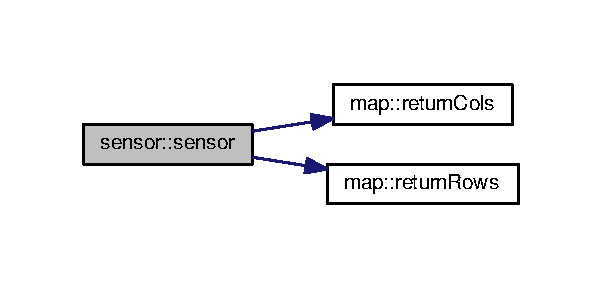
\includegraphics[width=289pt]{classsensor_af1db958929faf6e927e2eca5b05c3b40_cgraph}
\end{center}
\end{figure}


\index{sensor@{sensor}!````~sensor@{$\sim$sensor}}
\index{````~sensor@{$\sim$sensor}!sensor@{sensor}}
\subsubsection[{\texorpdfstring{$\sim$sensor()}{~sensor()}}]{\setlength{\rightskip}{0pt plus 5cm}sensor\+::$\sim$sensor (
\begin{DoxyParamCaption}
{}
\end{DoxyParamCaption}
)}\hypertarget{classsensor_a9252346748c0bd090109ee5bcf45f13a}{}\label{classsensor_a9252346748c0bd090109ee5bcf45f13a}


Definition at line 90 of file sensor.\+cpp.



\subsection{Member Function Documentation}
\index{sensor@{sensor}!get\+Radiation\+Map@{get\+Radiation\+Map}}
\index{get\+Radiation\+Map@{get\+Radiation\+Map}!sensor@{sensor}}
\subsubsection[{\texorpdfstring{get\+Radiation\+Map()}{getRadiationMap()}}]{\setlength{\rightskip}{0pt plus 5cm}std\+::vector$<$ std\+::vector$<$ float $>$ $>$ sensor\+::get\+Radiation\+Map (
\begin{DoxyParamCaption}
{}
\end{DoxyParamCaption}
)}\hypertarget{classsensor_af13c7b147a19c868375b44199ab9760e}{}\label{classsensor_af13c7b147a19c868375b44199ab9760e}


Class to implement the \hyperlink{classBFS}{B\+FS}. 

\begin{DoxyReturn}{Returns}
radiation\+Map in 2-\/D vector 
\end{DoxyReturn}


Definition at line 86 of file sensor.\+cpp.



References radiation\+Map.



Referenced by T\+E\+S\+T().

\index{sensor@{sensor}!save\+Radiation\+Map@{save\+Radiation\+Map}}
\index{save\+Radiation\+Map@{save\+Radiation\+Map}!sensor@{sensor}}
\subsubsection[{\texorpdfstring{save\+Radiation\+Map()}{saveRadiationMap()}}]{\setlength{\rightskip}{0pt plus 5cm}void sensor\+::save\+Radiation\+Map (
\begin{DoxyParamCaption}
{}
\end{DoxyParamCaption}
)}\hypertarget{classsensor_aa7aac0b5dca04e72e9334457a3cbd498}{}\label{classsensor_aa7aac0b5dca04e72e9334457a3cbd498}


Class to save the radiation data as ppm file. 

\begin{DoxyReturn}{Returns}
None 
\end{DoxyReturn}


Definition at line 65 of file sensor.\+cpp.



References radiation\+Map.



Referenced by main().



\subsection{Member Data Documentation}
\index{sensor@{sensor}!radiation\+Map@{radiation\+Map}}
\index{radiation\+Map@{radiation\+Map}!sensor@{sensor}}
\subsubsection[{\texorpdfstring{radiation\+Map}{radiationMap}}]{\setlength{\rightskip}{0pt plus 5cm}std\+::vector$<$std\+::vector$<$float$>$ $>$ sensor\+::radiation\+Map\hspace{0.3cm}{\ttfamily [private]}}\hypertarget{classsensor_a20a26da767dcc2547c02e56dc969e549}{}\label{classsensor_a20a26da767dcc2547c02e56dc969e549}


Definition at line 56 of file sensor.\+hpp.



Referenced by get\+Radiation\+Map(), save\+Radiation\+Map(), and sensor().



The documentation for this class was generated from the following files\+:\begin{DoxyCompactItemize}
\item 
include/\hyperlink{sensor_8hpp}{sensor.\+hpp}\item 
src/\hyperlink{sensor_8cpp}{sensor.\+cpp}\end{DoxyCompactItemize}

\chapter{File Documentation}
\hypertarget{BFS_8hpp}{}\section{include/\+B\+FS.hpp File Reference}
\label{BFS_8hpp}\index{include/\+B\+F\+S.\+hpp@{include/\+B\+F\+S.\+hpp}}


To declare a class which implements \hyperlink{classBFS}{B\+FS}  Nantha Kumar Sunder  Nithish Sanjeev Kumar.  


{\ttfamily \#include $<$vector$>$}\\*
{\ttfamily \#include $<$queue$>$}\\*
{\ttfamily \#include \char`\"{}ros/ros.\+h\char`\"{}}\\*
Include dependency graph for B\+F\+S.\+hpp\+:
\nopagebreak
\begin{figure}[H]
\begin{center}
\leavevmode
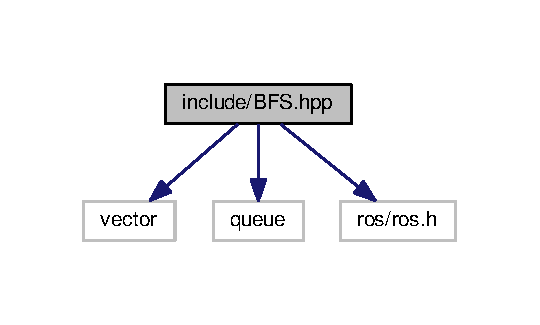
\includegraphics[width=259pt]{BFS_8hpp__incl}
\end{center}
\end{figure}
This graph shows which files directly or indirectly include this file\+:
\nopagebreak
\begin{figure}[H]
\begin{center}
\leavevmode
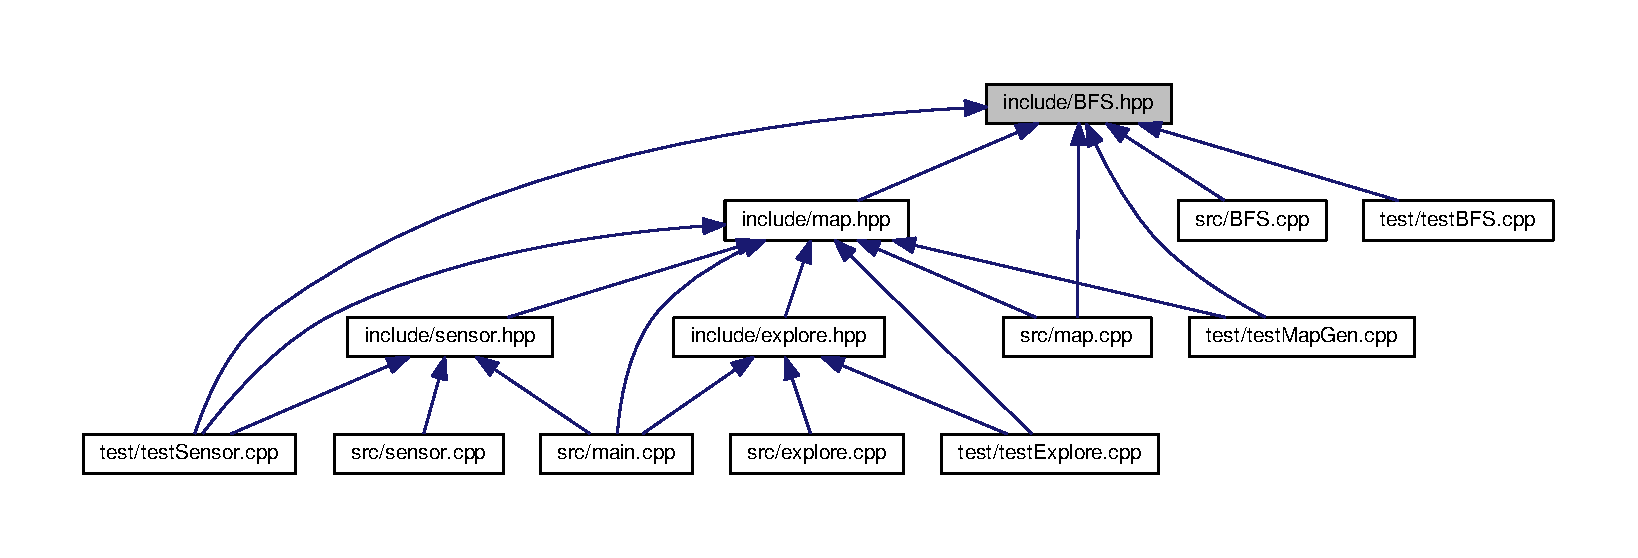
\includegraphics[width=350pt]{BFS_8hpp__dep__incl}
\end{center}
\end{figure}
\subsection*{Classes}
\begin{DoxyCompactItemize}
\item 
class \hyperlink{classBFS}{B\+FS}
\begin{DoxyCompactList}\small\item\em Class to implement the \hyperlink{classBFS}{B\+FS}. \end{DoxyCompactList}\end{DoxyCompactItemize}


\subsection{Detailed Description}
To declare a class which implements \hyperlink{classBFS}{B\+FS}  Nantha Kumar Sunder  Nithish Sanjeev Kumar. 

B\+SD 3-\/\+Clause License

Copyright (c) 2018, Nantha Kumar Sunder, Nithish Sanjeev Kumar All rights reserved.

Redistribution and use in source and binary forms, with or without modification, are permitted provided that the following conditions are met\+:


\begin{DoxyItemize}
\item Redistributions of source code must retain the above copyright notice, this list of conditions and the following disclaimer.
\item Redistributions in binary form must reproduce the above copyright notice, this list of conditions and the following disclaimer in the documentation and/or other materials provided with the distribution.
\item Neither the name of the copyright holder nor the names of its contributors may be used to endorse or promote products derived from this software without specific prior written permission.
\end{DoxyItemize}

T\+H\+IS S\+O\+F\+T\+W\+A\+RE IS P\+R\+O\+V\+I\+D\+ED BY T\+HE C\+O\+P\+Y\+R\+I\+G\+HT H\+O\+L\+D\+E\+RS A\+ND C\+O\+N\+T\+R\+I\+B\+U\+T\+O\+RS \char`\"{}\+A\+S I\+S\char`\"{} A\+ND A\+NY E\+X\+P\+R\+E\+SS OR I\+M\+P\+L\+I\+ED W\+A\+R\+R\+A\+N\+T\+I\+ES, I\+N\+C\+L\+U\+D\+I\+NG, B\+UT N\+OT L\+I\+M\+I\+T\+ED TO, T\+HE I\+M\+P\+L\+I\+ED W\+A\+R\+R\+A\+N\+T\+I\+ES OF M\+E\+R\+C\+H\+A\+N\+T\+A\+B\+I\+L\+I\+TY A\+ND F\+I\+T\+N\+E\+SS F\+OR A P\+A\+R\+T\+I\+C\+U\+L\+AR P\+U\+R\+P\+O\+SE A\+RE D\+I\+S\+C\+L\+A\+I\+M\+ED. IN NO E\+V\+E\+NT S\+H\+A\+LL T\+HE C\+O\+P\+Y\+R\+I\+G\+HT H\+O\+L\+D\+ER OR C\+O\+N\+T\+R\+I\+B\+U\+T\+O\+RS BE L\+I\+A\+B\+LE F\+OR A\+NY D\+I\+R\+E\+CT, I\+N\+D\+I\+R\+E\+CT, I\+N\+C\+I\+D\+E\+N\+T\+AL, S\+P\+E\+C\+I\+AL, E\+X\+E\+M\+P\+L\+A\+RY, OR C\+O\+N\+S\+E\+Q\+U\+E\+N\+T\+I\+AL D\+A\+M\+A\+G\+ES (I\+N\+C\+L\+U\+D\+I\+NG, B\+UT N\+OT L\+I\+M\+I\+T\+ED TO, P\+R\+O\+C\+U\+R\+E\+M\+E\+NT OF S\+U\+B\+S\+T\+I\+T\+U\+TE G\+O\+O\+DS OR S\+E\+R\+V\+I\+C\+ES; L\+O\+SS OF U\+SE, D\+A\+TA, OR P\+R\+O\+F\+I\+TS; OR B\+U\+S\+I\+N\+E\+SS I\+N\+T\+E\+R\+R\+U\+P\+T\+I\+ON) H\+O\+W\+E\+V\+ER C\+A\+U\+S\+ED A\+ND ON A\+NY T\+H\+E\+O\+RY OF L\+I\+A\+B\+I\+L\+I\+TY, W\+H\+E\+T\+H\+ER IN C\+O\+N\+T\+R\+A\+CT, S\+T\+R\+I\+CT L\+I\+A\+B\+I\+L\+I\+TY, OR T\+O\+RT (I\+N\+C\+L\+U\+D\+I\+NG N\+E\+G\+L\+I\+G\+E\+N\+CE OR O\+T\+H\+E\+R\+W\+I\+SE) A\+R\+I\+S\+I\+NG IN A\+NY W\+AY O\+UT OF T\+HE U\+SE OF T\+H\+IS S\+O\+F\+T\+W\+A\+RE, E\+V\+EN IF A\+D\+V\+I\+S\+ED OF T\+HE P\+O\+S\+S\+I\+B\+I\+L\+I\+TY OF S\+U\+CH D\+A\+M\+A\+GE. \begin{DoxyCopyright}{Copyright}
2018 , Nantha Kumar Sunder, Nithish Sanjeev Kumar All rights reserved 
\end{DoxyCopyright}

\hypertarget{explore_8hpp}{}\section{include/explore.hpp File Reference}
\label{explore_8hpp}\index{include/explore.\+hpp@{include/explore.\+hpp}}


a class to explores the map  


{\ttfamily \#include $<$queue$>$}\\*
{\ttfamily \#include $<$vector$>$}\\*
{\ttfamily \#include \char`\"{}map.\+hpp\char`\"{}}\\*
Include dependency graph for explore.\+hpp\+:
\nopagebreak
\begin{figure}[H]
\begin{center}
\leavevmode
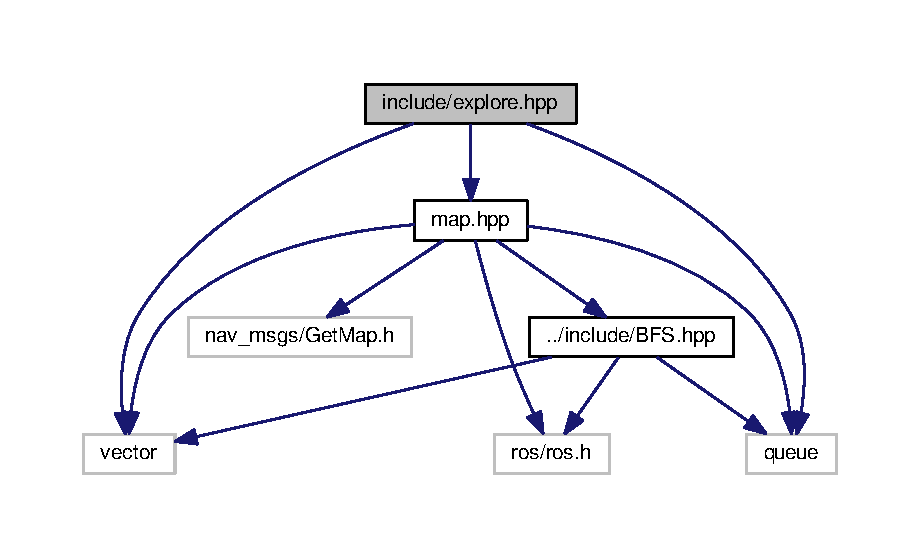
\includegraphics[width=350pt]{explore_8hpp__incl}
\end{center}
\end{figure}
This graph shows which files directly or indirectly include this file\+:
\nopagebreak
\begin{figure}[H]
\begin{center}
\leavevmode
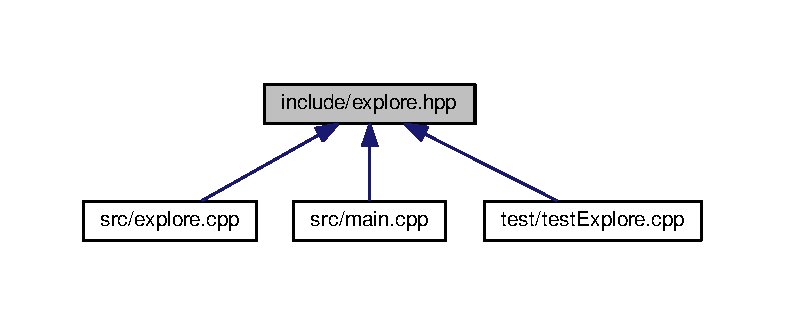
\includegraphics[width=350pt]{explore_8hpp__dep__incl}
\end{center}
\end{figure}
\subsection*{Classes}
\begin{DoxyCompactItemize}
\item 
class \hyperlink{classexplore}{explore}
\begin{DoxyCompactList}\small\item\em Class to implement the \hyperlink{classBFS}{B\+FS}. \end{DoxyCompactList}\end{DoxyCompactItemize}


\subsection{Detailed Description}
a class to explores the map 

B\+SD 3-\/\+Clause License

Copyright (c) 2018, Nantha Kumar Sunder, Nithish Sanjeev Kumar All rights reserved.

Redistribution and use in source and binary forms, with or without modification, are permitted provided that the following conditions are met\+:


\begin{DoxyItemize}
\item Redistributions of source code must retain the above copyright notice, this list of conditions and the following disclaimer.
\item Redistributions in binary form must reproduce the above copyright notice, this list of conditions and the following disclaimer in the documentation and/or other materials provided with the distribution.
\item Neither the name of the copyright holder nor the names of its contributors may be used to endorse or promote products derived from this software without specific prior written permission.
\end{DoxyItemize}

T\+H\+IS S\+O\+F\+T\+W\+A\+RE IS P\+R\+O\+V\+I\+D\+ED BY T\+HE C\+O\+P\+Y\+R\+I\+G\+HT H\+O\+L\+D\+E\+RS A\+ND C\+O\+N\+T\+R\+I\+B\+U\+T\+O\+RS \char`\"{}\+A\+S I\+S\char`\"{} A\+ND A\+NY E\+X\+P\+R\+E\+SS OR I\+M\+P\+L\+I\+ED W\+A\+R\+R\+A\+N\+T\+I\+ES, I\+N\+C\+L\+U\+D\+I\+NG, B\+UT N\+OT L\+I\+M\+I\+T\+ED TO, T\+HE I\+M\+P\+L\+I\+ED W\+A\+R\+R\+A\+N\+T\+I\+ES OF M\+E\+R\+C\+H\+A\+N\+T\+A\+B\+I\+L\+I\+TY A\+ND F\+I\+T\+N\+E\+SS F\+OR A P\+A\+R\+T\+I\+C\+U\+L\+AR P\+U\+R\+P\+O\+SE A\+RE D\+I\+S\+C\+L\+A\+I\+M\+ED. IN NO E\+V\+E\+NT S\+H\+A\+LL T\+HE C\+O\+P\+Y\+R\+I\+G\+HT H\+O\+L\+D\+ER OR C\+O\+N\+T\+R\+I\+B\+U\+T\+O\+RS BE L\+I\+A\+B\+LE F\+OR A\+NY D\+I\+R\+E\+CT, I\+N\+D\+I\+R\+E\+CT, I\+N\+C\+I\+D\+E\+N\+T\+AL, S\+P\+E\+C\+I\+AL, E\+X\+E\+M\+P\+L\+A\+RY, OR C\+O\+N\+S\+E\+Q\+U\+E\+N\+T\+I\+AL D\+A\+M\+A\+G\+ES (I\+N\+C\+L\+U\+D\+I\+NG, B\+UT N\+OT L\+I\+M\+I\+T\+ED TO, P\+R\+O\+C\+U\+R\+E\+M\+E\+NT OF S\+U\+B\+S\+T\+I\+T\+U\+TE G\+O\+O\+DS OR S\+E\+R\+V\+I\+C\+ES; L\+O\+SS OF U\+SE, D\+A\+TA, OR P\+R\+O\+F\+I\+TS; OR B\+U\+S\+I\+N\+E\+SS I\+N\+T\+E\+R\+R\+U\+P\+T\+I\+ON) H\+O\+W\+E\+V\+ER C\+A\+U\+S\+ED A\+ND ON A\+NY T\+H\+E\+O\+RY OF L\+I\+A\+B\+I\+L\+I\+TY, W\+H\+E\+T\+H\+ER IN C\+O\+N\+T\+R\+A\+CT, S\+T\+R\+I\+CT L\+I\+A\+B\+I\+L\+I\+TY, OR T\+O\+RT (I\+N\+C\+L\+U\+D\+I\+NG N\+E\+G\+L\+I\+G\+E\+N\+CE OR O\+T\+H\+E\+R\+W\+I\+SE) A\+R\+I\+S\+I\+NG IN A\+NY W\+AY O\+UT OF T\+HE U\+SE OF T\+H\+IS S\+O\+F\+T\+W\+A\+RE, E\+V\+EN IF A\+D\+V\+I\+S\+ED OF T\+HE P\+O\+S\+S\+I\+B\+I\+L\+I\+TY OF S\+U\+CH D\+A\+M\+A\+GE.

Nantha Kumar Sunder  Nithish Sanjeev Kumar \begin{DoxyCopyright}{Copyright}
2018 , Nantha Kumar Sunder, Nithish Sanjeev Kumar All rights reserved 
\end{DoxyCopyright}

\hypertarget{map_8hpp}{}\section{include/map.hpp File Reference}
\label{map_8hpp}\index{include/map.\+hpp@{include/map.\+hpp}}


To declare a class which implements the map and processes the frontier.  


{\ttfamily \#include $<$ros/ros.\+h$>$}\\*
{\ttfamily \#include $<$nav\+\_\+msgs/\+Get\+Map.\+h$>$}\\*
{\ttfamily \#include $<$vector$>$}\\*
{\ttfamily \#include $<$queue$>$}\\*
{\ttfamily \#include \char`\"{}../include/\+B\+F\+S.\+hpp\char`\"{}}\\*
Include dependency graph for map.\+hpp\+:
\nopagebreak
\begin{figure}[H]
\begin{center}
\leavevmode
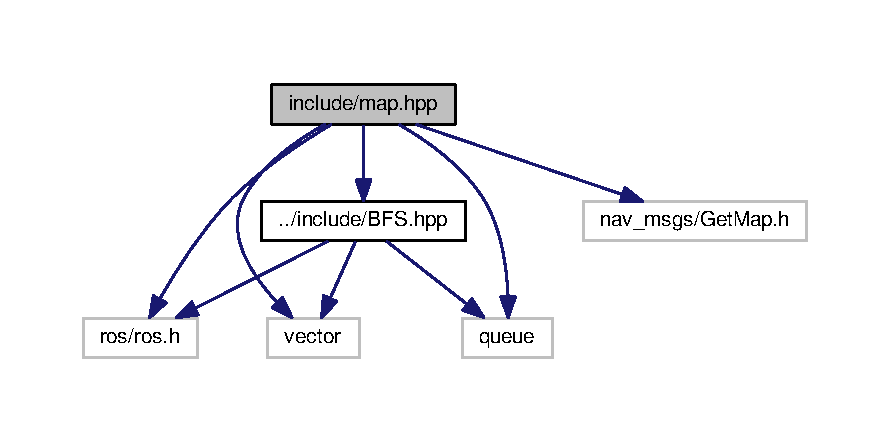
\includegraphics[width=350pt]{map_8hpp__incl}
\end{center}
\end{figure}
This graph shows which files directly or indirectly include this file\+:
\nopagebreak
\begin{figure}[H]
\begin{center}
\leavevmode
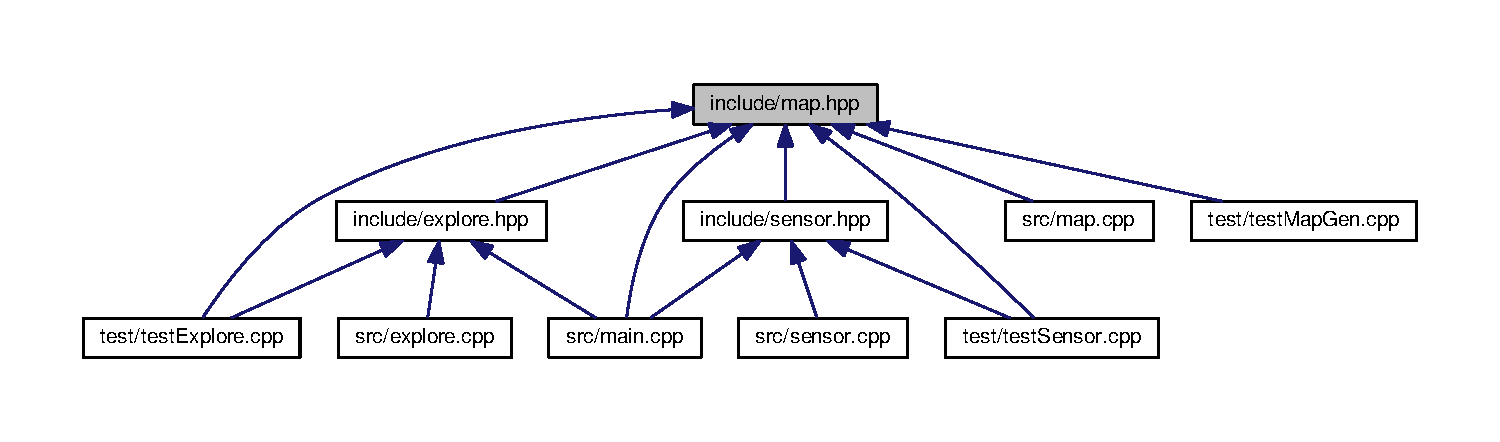
\includegraphics[width=350pt]{map_8hpp__dep__incl}
\end{center}
\end{figure}
\subsection*{Classes}
\begin{DoxyCompactItemize}
\item 
class \hyperlink{classmap}{map}
\begin{DoxyCompactList}\small\item\em Class to implement the M\+AP. \end{DoxyCompactList}\end{DoxyCompactItemize}


\subsection{Detailed Description}
To declare a class which implements the map and processes the frontier. 

B\+SD 3-\/\+Clause License

Copyright (c) 2018, Nantha Kumar Sunder, Nithish Sanjeev Kumar All rights reserved.

Redistribution and use in source and binary forms, with or without modification, are permitted provided that the following conditions are met\+:


\begin{DoxyItemize}
\item Redistributions of source code must retain the above copyright notice, this list of conditions and the following disclaimer.
\item Redistributions in binary form must reproduce the above copyright notice, this list of conditions and the following disclaimer in the documentation and/or other materials provided with the distribution.
\item Neither the name of the copyright holder nor the names of its contributors may be used to endorse or promote products derived from this software without specific prior written permission.
\end{DoxyItemize}

T\+H\+IS S\+O\+F\+T\+W\+A\+RE IS P\+R\+O\+V\+I\+D\+ED BY T\+HE C\+O\+P\+Y\+R\+I\+G\+HT H\+O\+L\+D\+E\+RS A\+ND C\+O\+N\+T\+R\+I\+B\+U\+T\+O\+RS \char`\"{}\+A\+S I\+S\char`\"{} A\+ND A\+NY E\+X\+P\+R\+E\+SS OR I\+M\+P\+L\+I\+ED W\+A\+R\+R\+A\+N\+T\+I\+ES, I\+N\+C\+L\+U\+D\+I\+NG, B\+UT N\+OT L\+I\+M\+I\+T\+ED TO, T\+HE I\+M\+P\+L\+I\+ED W\+A\+R\+R\+A\+N\+T\+I\+ES OF M\+E\+R\+C\+H\+A\+N\+T\+A\+B\+I\+L\+I\+TY A\+ND F\+I\+T\+N\+E\+SS F\+OR A P\+A\+R\+T\+I\+C\+U\+L\+AR P\+U\+R\+P\+O\+SE A\+RE D\+I\+S\+C\+L\+A\+I\+M\+ED. IN NO E\+V\+E\+NT S\+H\+A\+LL T\+HE C\+O\+P\+Y\+R\+I\+G\+HT H\+O\+L\+D\+ER OR C\+O\+N\+T\+R\+I\+B\+U\+T\+O\+RS BE L\+I\+A\+B\+LE F\+OR A\+NY D\+I\+R\+E\+CT, I\+N\+D\+I\+R\+E\+CT, I\+N\+C\+I\+D\+E\+N\+T\+AL, S\+P\+E\+C\+I\+AL, E\+X\+E\+M\+P\+L\+A\+RY, OR C\+O\+N\+S\+E\+Q\+U\+E\+N\+T\+I\+AL D\+A\+M\+A\+G\+ES (I\+N\+C\+L\+U\+D\+I\+NG, B\+UT N\+OT L\+I\+M\+I\+T\+ED TO, P\+R\+O\+C\+U\+R\+E\+M\+E\+NT OF S\+U\+B\+S\+T\+I\+T\+U\+TE G\+O\+O\+DS OR S\+E\+R\+V\+I\+C\+ES; L\+O\+SS OF U\+SE, D\+A\+TA, OR P\+R\+O\+F\+I\+TS; OR B\+U\+S\+I\+N\+E\+SS I\+N\+T\+E\+R\+R\+U\+P\+T\+I\+ON) H\+O\+W\+E\+V\+ER C\+A\+U\+S\+ED A\+ND ON A\+NY T\+H\+E\+O\+RY OF L\+I\+A\+B\+I\+L\+I\+TY, W\+H\+E\+T\+H\+ER IN C\+O\+N\+T\+R\+A\+CT, S\+T\+R\+I\+CT L\+I\+A\+B\+I\+L\+I\+TY, OR T\+O\+RT (I\+N\+C\+L\+U\+D\+I\+NG N\+E\+G\+L\+I\+G\+E\+N\+CE OR O\+T\+H\+E\+R\+W\+I\+SE) A\+R\+I\+S\+I\+NG IN A\+NY W\+AY O\+UT OF T\+HE U\+SE OF T\+H\+IS S\+O\+F\+T\+W\+A\+RE, E\+V\+EN IF A\+D\+V\+I\+S\+ED OF T\+HE P\+O\+S\+S\+I\+B\+I\+L\+I\+TY OF S\+U\+CH D\+A\+M\+A\+GE.

Nithish Sanjeev Kumar  Nantha Kumar Sunder \begin{DoxyCopyright}{Copyright}
2018 , Nantha Kumar Sunder, Nithish Sanjeev Kumar All rights reserved 
\end{DoxyCopyright}

\hypertarget{sensor_8hpp}{}\section{include/sensor.hpp File Reference}
\label{sensor_8hpp}\index{include/sensor.\+hpp@{include/sensor.\+hpp}}


To declare a class which implements radiation sensor module.  


{\ttfamily \#include $<$vector$>$}\\*
{\ttfamily \#include \char`\"{}map.\+hpp\char`\"{}}\\*
Include dependency graph for sensor.\+hpp\+:
\nopagebreak
\begin{figure}[H]
\begin{center}
\leavevmode
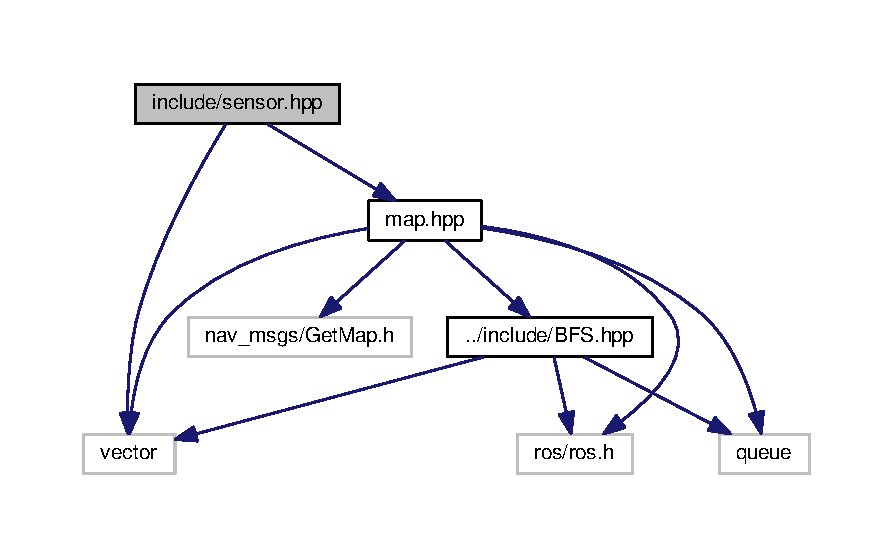
\includegraphics[width=350pt]{sensor_8hpp__incl}
\end{center}
\end{figure}
This graph shows which files directly or indirectly include this file\+:
\nopagebreak
\begin{figure}[H]
\begin{center}
\leavevmode
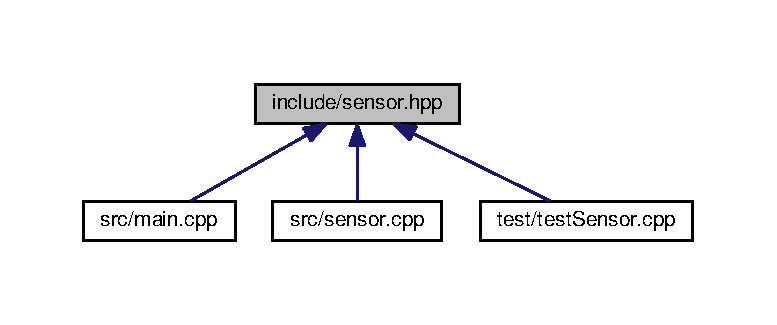
\includegraphics[width=350pt]{sensor_8hpp__dep__incl}
\end{center}
\end{figure}
\subsection*{Classes}
\begin{DoxyCompactItemize}
\item 
class \hyperlink{classsensor}{sensor}
\begin{DoxyCompactList}\small\item\em Class to implement the radiation sensor. \end{DoxyCompactList}\end{DoxyCompactItemize}


\subsection{Detailed Description}
To declare a class which implements radiation sensor module. 

class definition which implements radiation sensor module

B\+SD 3-\/\+Clause License

Copyright (c) 2018, Nantha Kumar Sunder, Nithish Sanjeev Kumar All rights reserved.

Redistribution and use in source and binary forms, with or without modification, are permitted provided that the following conditions are met\+:


\begin{DoxyItemize}
\item Redistributions of source code must retain the above copyright notice, this list of conditions and the following disclaimer.
\item Redistributions in binary form must reproduce the above copyright notice, this list of conditions and the following disclaimer in the documentation and/or other materials provided with the distribution.
\item Neither the name of the copyright holder nor the names of its contributors may be used to endorse or promote products derived from this software without specific prior written permission.
\end{DoxyItemize}

T\+H\+IS S\+O\+F\+T\+W\+A\+RE IS P\+R\+O\+V\+I\+D\+ED BY T\+HE C\+O\+P\+Y\+R\+I\+G\+HT H\+O\+L\+D\+E\+RS A\+ND C\+O\+N\+T\+R\+I\+B\+U\+T\+O\+RS \char`\"{}\+A\+S I\+S\char`\"{} A\+ND A\+NY E\+X\+P\+R\+E\+SS OR I\+M\+P\+L\+I\+ED W\+A\+R\+R\+A\+N\+T\+I\+ES, I\+N\+C\+L\+U\+D\+I\+NG, B\+UT N\+OT L\+I\+M\+I\+T\+ED TO, T\+HE I\+M\+P\+L\+I\+ED W\+A\+R\+R\+A\+N\+T\+I\+ES OF M\+E\+R\+C\+H\+A\+N\+T\+A\+B\+I\+L\+I\+TY A\+ND F\+I\+T\+N\+E\+SS F\+OR A P\+A\+R\+T\+I\+C\+U\+L\+AR P\+U\+R\+P\+O\+SE A\+RE D\+I\+S\+C\+L\+A\+I\+M\+ED. IN NO E\+V\+E\+NT S\+H\+A\+LL T\+HE C\+O\+P\+Y\+R\+I\+G\+HT H\+O\+L\+D\+ER OR C\+O\+N\+T\+R\+I\+B\+U\+T\+O\+RS BE L\+I\+A\+B\+LE F\+OR A\+NY D\+I\+R\+E\+CT, I\+N\+D\+I\+R\+E\+CT, I\+N\+C\+I\+D\+E\+N\+T\+AL, S\+P\+E\+C\+I\+AL, E\+X\+E\+M\+P\+L\+A\+RY, OR C\+O\+N\+S\+E\+Q\+U\+E\+N\+T\+I\+AL D\+A\+M\+A\+G\+ES (I\+N\+C\+L\+U\+D\+I\+NG, B\+UT N\+OT L\+I\+M\+I\+T\+ED TO, P\+R\+O\+C\+U\+R\+E\+M\+E\+NT OF S\+U\+B\+S\+T\+I\+T\+U\+TE G\+O\+O\+DS OR S\+E\+R\+V\+I\+C\+ES; L\+O\+SS OF U\+SE, D\+A\+TA, OR P\+R\+O\+F\+I\+TS; OR B\+U\+S\+I\+N\+E\+SS I\+N\+T\+E\+R\+R\+U\+P\+T\+I\+ON) H\+O\+W\+E\+V\+ER C\+A\+U\+S\+ED A\+ND ON A\+NY T\+H\+E\+O\+RY OF L\+I\+A\+B\+I\+L\+I\+TY, W\+H\+E\+T\+H\+ER IN C\+O\+N\+T\+R\+A\+CT, S\+T\+R\+I\+CT L\+I\+A\+B\+I\+L\+I\+TY, OR T\+O\+RT (I\+N\+C\+L\+U\+D\+I\+NG N\+E\+G\+L\+I\+G\+E\+N\+CE OR O\+T\+H\+E\+R\+W\+I\+SE) A\+R\+I\+S\+I\+NG IN A\+NY W\+AY O\+UT OF T\+HE U\+SE OF T\+H\+IS S\+O\+F\+T\+W\+A\+RE, E\+V\+EN IF A\+D\+V\+I\+S\+ED OF T\+HE P\+O\+S\+S\+I\+B\+I\+L\+I\+TY OF S\+U\+CH D\+A\+M\+A\+GE.

Nantha Kumar Sunder  Nithish Sanjeev Kumar \begin{DoxyCopyright}{Copyright}
2018 , Nantha Kumar Sunder, Nithish Sanjeev Kumar All rights reserved 
\end{DoxyCopyright}

\hypertarget{BFS_8cpp}{}\section{src/\+B\+FS.cpp File Reference}
\label{BFS_8cpp}\index{src/\+B\+F\+S.\+cpp@{src/\+B\+F\+S.\+cpp}}
{\ttfamily \#include $<$ros/ros.\+h$>$}\\*
{\ttfamily \#include $<$queue$>$}\\*
{\ttfamily \#include $<$vector$>$}\\*
{\ttfamily \#include \char`\"{}B\+F\+S.\+hpp\char`\"{}}\\*
Include dependency graph for B\+F\+S.\+cpp\+:
\nopagebreak
\begin{figure}[H]
\begin{center}
\leavevmode
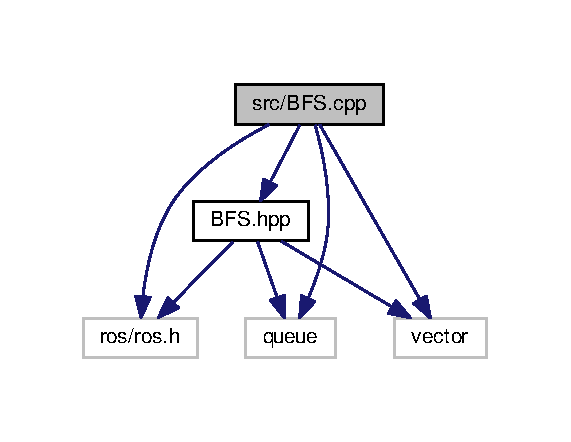
\includegraphics[width=274pt]{BFS_8cpp__incl}
\end{center}
\end{figure}

\hypertarget{explore_8cpp}{}\section{src/explore.cpp File Reference}
\label{explore_8cpp}\index{src/explore.\+cpp@{src/explore.\+cpp}}


To implement the function of the class \hyperlink{classBFS}{B\+FS}.  


{\ttfamily \#include $<$tf/transform\+\_\+broadcaster.\+h$>$}\\*
{\ttfamily \#include $<$tf/transform\+\_\+listener.\+h$>$}\\*
{\ttfamily \#include $<$cstdlib$>$}\\*
{\ttfamily \#include $<$algorithm$>$}\\*
{\ttfamily \#include \char`\"{}actionlib/client/simple\+\_\+action\+\_\+client.\+h\char`\"{}}\\*
{\ttfamily \#include \char`\"{}move\+\_\+base\+\_\+msgs/\+Move\+Base\+Action.\+h\char`\"{}}\\*
{\ttfamily \#include \char`\"{}geometry\+\_\+msgs/\+Twist.\+h\char`\"{}}\\*
{\ttfamily \#include \char`\"{}explore.\+hpp\char`\"{}}\\*
Include dependency graph for explore.\+cpp\+:
\nopagebreak
\begin{figure}[H]
\begin{center}
\leavevmode
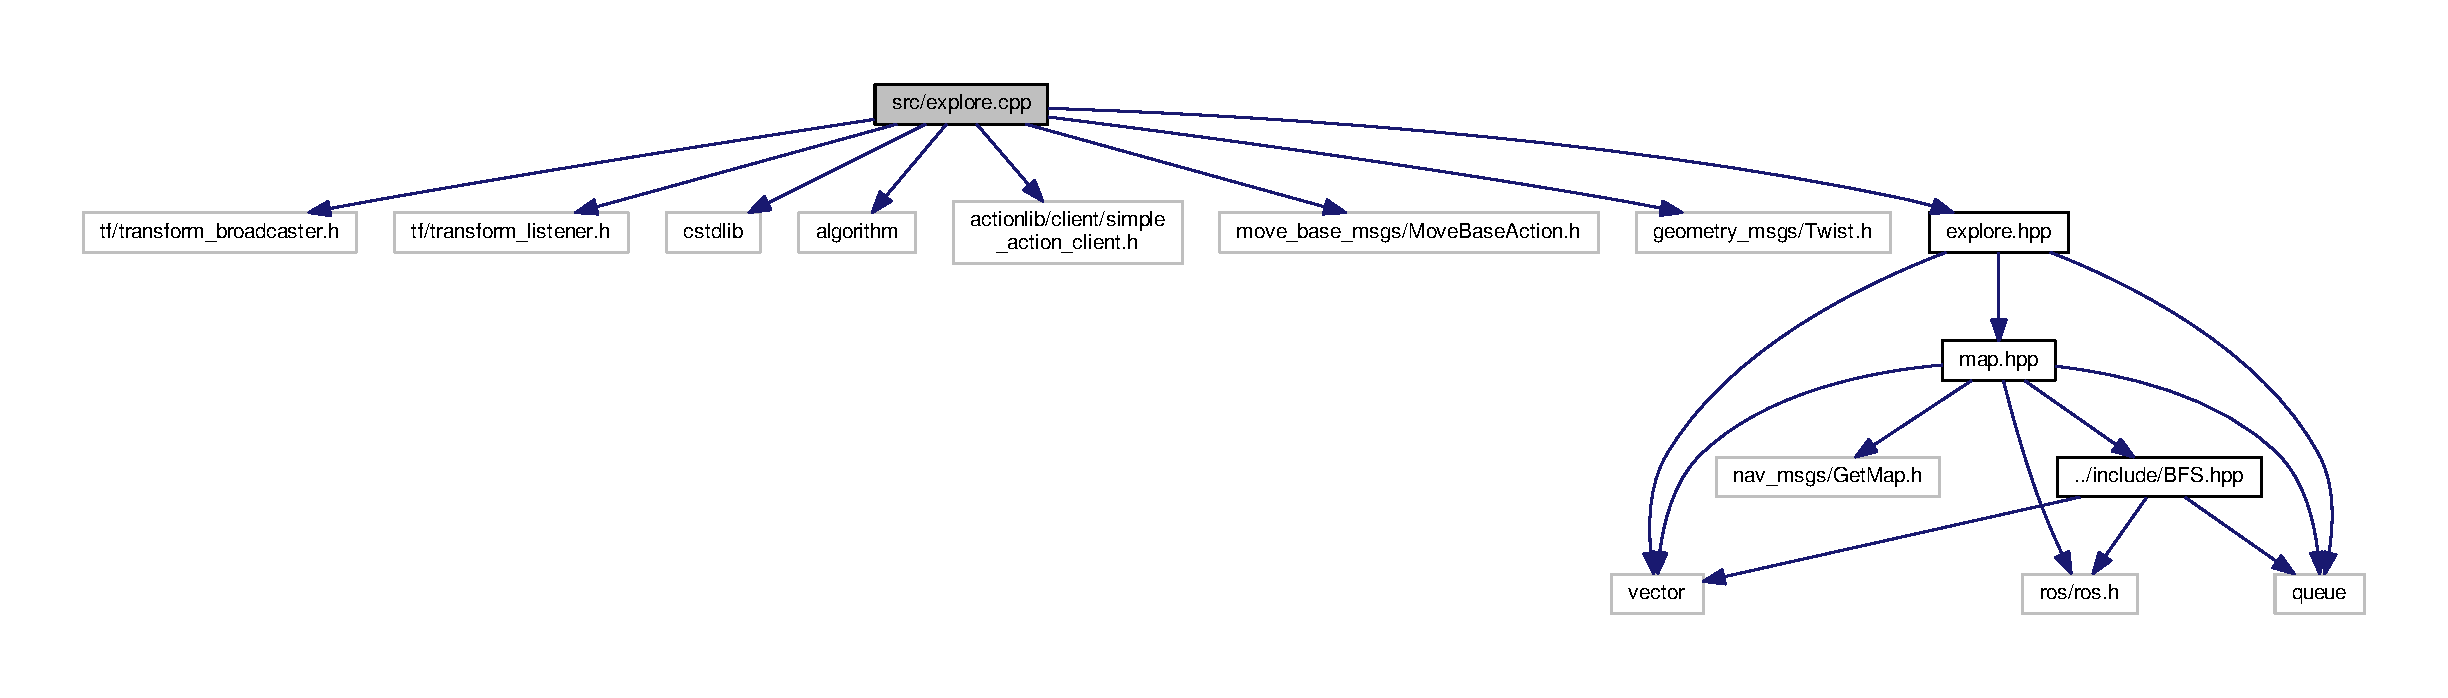
\includegraphics[width=350pt]{explore_8cpp__incl}
\end{center}
\end{figure}


\subsection{Detailed Description}
To implement the function of the class \hyperlink{classBFS}{B\+FS}. 

To implement the functions of the class explore.

B\+SD 3-\/\+Clause License

Copyright (c) 2018, Nantha Kumar Sunder, Nithish Sanjeev Kumar All rights reserved.

Redistribution and use in source and binary forms, with or without modification, are permitted provided that the following conditions are met\+:


\begin{DoxyItemize}
\item Redistributions of source code must retain the above copyright notice, this list of conditions and the following disclaimer.
\item Redistributions in binary form must reproduce the above copyright notice, this list of conditions and the following disclaimer in the documentation and/or other materials provided with the distribution.
\item Neither the name of the copyright holder nor the names of its contributors may be used to endorse or promote products derived from this software without specific prior written permission.
\end{DoxyItemize}

T\+H\+IS S\+O\+F\+T\+W\+A\+RE IS P\+R\+O\+V\+I\+D\+ED BY T\+HE C\+O\+P\+Y\+R\+I\+G\+HT H\+O\+L\+D\+E\+RS A\+ND C\+O\+N\+T\+R\+I\+B\+U\+T\+O\+RS \char`\"{}\+A\+S I\+S\char`\"{} A\+ND A\+NY E\+X\+P\+R\+E\+SS OR I\+M\+P\+L\+I\+ED W\+A\+R\+R\+A\+N\+T\+I\+ES, I\+N\+C\+L\+U\+D\+I\+NG, B\+UT N\+OT L\+I\+M\+I\+T\+ED TO, T\+HE I\+M\+P\+L\+I\+ED W\+A\+R\+R\+A\+N\+T\+I\+ES OF M\+E\+R\+C\+H\+A\+N\+T\+A\+B\+I\+L\+I\+TY A\+ND F\+I\+T\+N\+E\+SS F\+OR A P\+A\+R\+T\+I\+C\+U\+L\+AR P\+U\+R\+P\+O\+SE A\+RE D\+I\+S\+C\+L\+A\+I\+M\+ED. IN NO E\+V\+E\+NT S\+H\+A\+LL T\+HE C\+O\+P\+Y\+R\+I\+G\+HT H\+O\+L\+D\+ER OR C\+O\+N\+T\+R\+I\+B\+U\+T\+O\+RS BE L\+I\+A\+B\+LE F\+OR A\+NY D\+I\+R\+E\+CT, I\+N\+D\+I\+R\+E\+CT, I\+N\+C\+I\+D\+E\+N\+T\+AL, S\+P\+E\+C\+I\+AL, E\+X\+E\+M\+P\+L\+A\+RY, OR C\+O\+N\+S\+E\+Q\+U\+E\+N\+T\+I\+AL D\+A\+M\+A\+G\+ES (I\+N\+C\+L\+U\+D\+I\+NG, B\+UT N\+OT L\+I\+M\+I\+T\+ED TO, P\+R\+O\+C\+U\+R\+E\+M\+E\+NT OF S\+U\+B\+S\+T\+I\+T\+U\+TE G\+O\+O\+DS OR S\+E\+R\+V\+I\+C\+ES; L\+O\+SS OF U\+SE, D\+A\+TA, OR P\+R\+O\+F\+I\+TS; OR B\+U\+S\+I\+N\+E\+SS I\+N\+T\+E\+R\+R\+U\+P\+T\+I\+ON) H\+O\+W\+E\+V\+ER C\+A\+U\+S\+ED A\+ND ON A\+NY T\+H\+E\+O\+RY OF L\+I\+A\+B\+I\+L\+I\+TY, W\+H\+E\+T\+H\+ER IN C\+O\+N\+T\+R\+A\+CT, S\+T\+R\+I\+CT L\+I\+A\+B\+I\+L\+I\+TY, OR T\+O\+RT (I\+N\+C\+L\+U\+D\+I\+NG N\+E\+G\+L\+I\+G\+E\+N\+CE OR O\+T\+H\+E\+R\+W\+I\+SE) A\+R\+I\+S\+I\+NG IN A\+NY W\+AY O\+UT OF T\+HE U\+SE OF T\+H\+IS S\+O\+F\+T\+W\+A\+RE, E\+V\+EN IF A\+D\+V\+I\+S\+ED OF T\+HE P\+O\+S\+S\+I\+B\+I\+L\+I\+TY OF S\+U\+CH D\+A\+M\+A\+GE.

Nantha Kumar Sunder  Nithish Sanjeev Kumar \begin{DoxyCopyright}{Copyright}
2018 , Nantha Kumar Sunder, Nithish Sanjeev Kumar All rights reserved 
\end{DoxyCopyright}

\hypertarget{src_2main_8cpp}{}\section{src/main.cpp File Reference}
\label{src_2main_8cpp}\index{src/main.\+cpp@{src/main.\+cpp}}
{\ttfamily \#include $<$ros/ros.\+h$>$}\\*
{\ttfamily \#include $<$stdlib.\+h$>$}\\*
{\ttfamily \#include $<$tf/transform\+\_\+broadcaster.\+h$>$}\\*
{\ttfamily \#include $<$tf/transform\+\_\+listener.\+h$>$}\\*
{\ttfamily \#include \char`\"{}geometry\+\_\+msgs/\+Twist.\+h\char`\"{}}\\*
{\ttfamily \#include \char`\"{}map.\+hpp\char`\"{}}\\*
{\ttfamily \#include \char`\"{}explore.\+hpp\char`\"{}}\\*
{\ttfamily \#include \char`\"{}sensor.\+hpp\char`\"{}}\\*
Include dependency graph for main.\+cpp\+:
\nopagebreak
\begin{figure}[H]
\begin{center}
\leavevmode
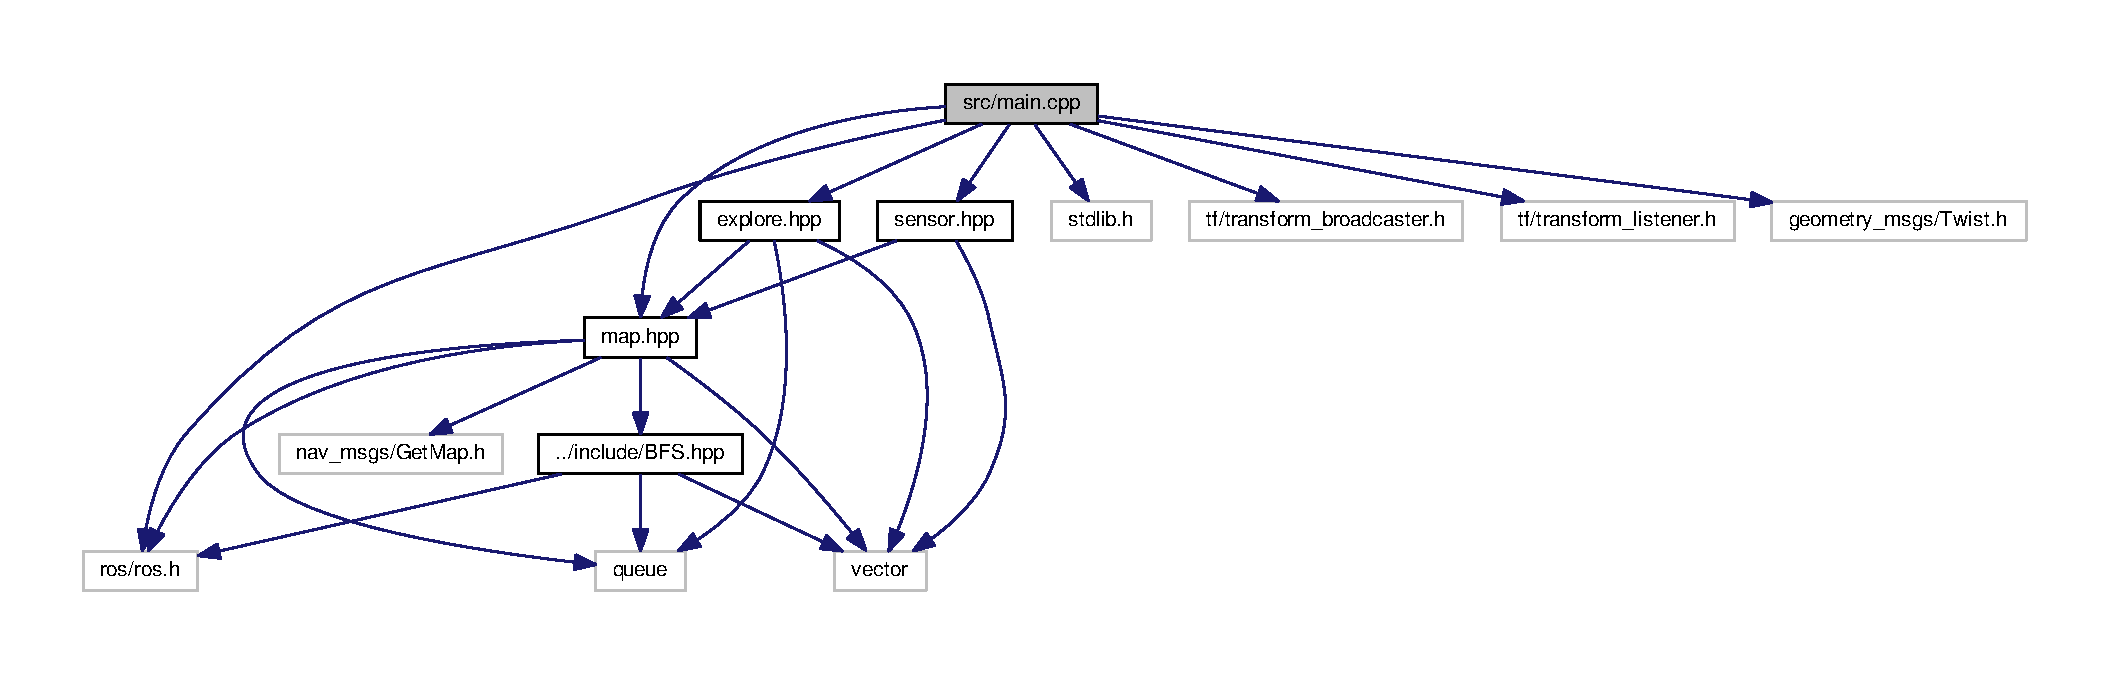
\includegraphics[width=350pt]{src_2main_8cpp__incl}
\end{center}
\end{figure}
\subsection*{Functions}
\begin{DoxyCompactItemize}
\item 
int \hyperlink{src_2main_8cpp_a3c04138a5bfe5d72780bb7e82a18e627}{main} (int argc, char $\ast$$\ast$argv)
\end{DoxyCompactItemize}


\subsection{Function Documentation}
\index{src/main.\+cpp@{src/main.\+cpp}!main@{main}}
\index{main@{main}!src/main.\+cpp@{src/main.\+cpp}}
\subsubsection[{\texorpdfstring{main(int argc, char $\ast$$\ast$argv)}{main(int argc, char **argv)}}]{\setlength{\rightskip}{0pt plus 5cm}int main (
\begin{DoxyParamCaption}
\item[{int}]{argc, }
\item[{char $\ast$$\ast$}]{argv}
\end{DoxyParamCaption}
)}\hypertarget{src_2main_8cpp_a3c04138a5bfe5d72780bb7e82a18e627}{}\label{src_2main_8cpp_a3c04138a5bfe5d72780bb7e82a18e627}


Definition at line 51 of file main.\+cpp.



References map\+::frontier\+Search(), map\+::get\+Resolution(), map\+::get\+Start(), explore\+::navigate(), map\+::nearest\+Centroid(), explore\+::path\+Search(), map\+::request\+Map(), map\+::return\+Cols(), map\+::return\+Rows(), and sensor\+::save\+Radiation\+Map().



Here is the call graph for this function\+:
\nopagebreak
\begin{figure}[H]
\begin{center}
\leavevmode
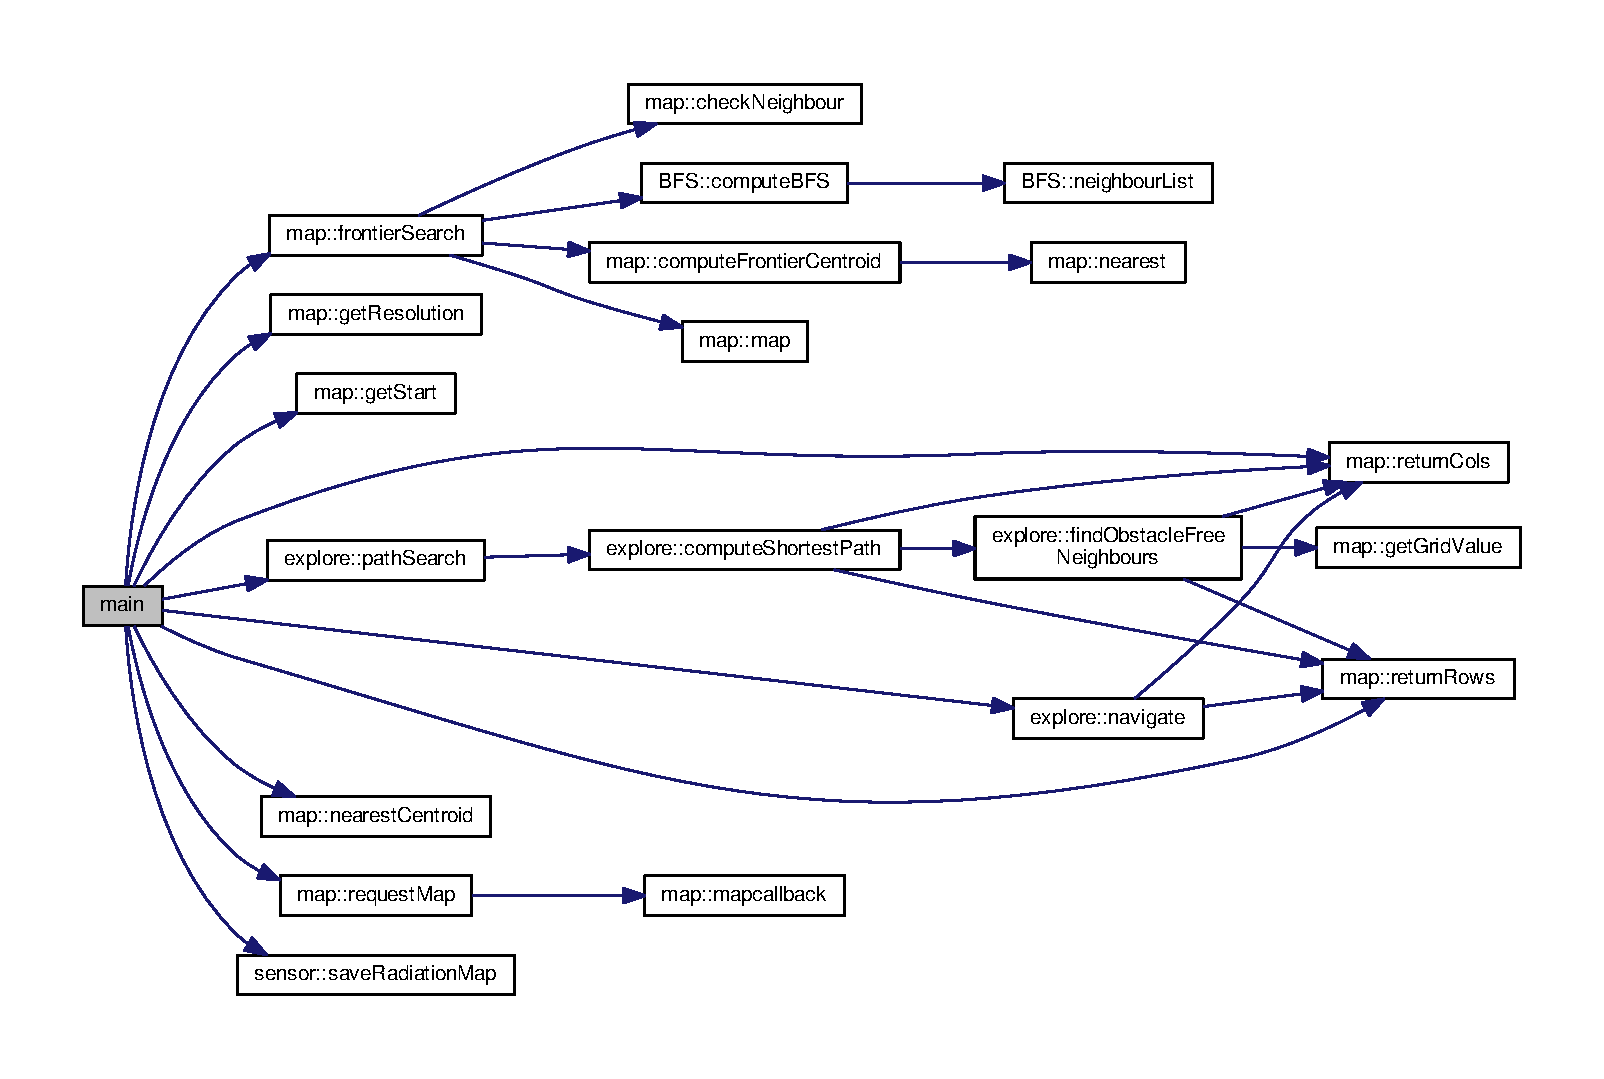
\includegraphics[width=350pt]{src_2main_8cpp_a3c04138a5bfe5d72780bb7e82a18e627_cgraph}
\end{center}
\end{figure}



\hypertarget{test_2main_8cpp}{}\section{test/main.cpp File Reference}
\label{test_2main_8cpp}\index{test/main.\+cpp@{test/main.\+cpp}}
{\ttfamily \#include $<$gtest/gtest.\+h$>$}\\*
{\ttfamily \#include $<$ros/ros.\+h$>$}\\*
Include dependency graph for main.\+cpp\+:
\nopagebreak
\begin{figure}[H]
\begin{center}
\leavevmode
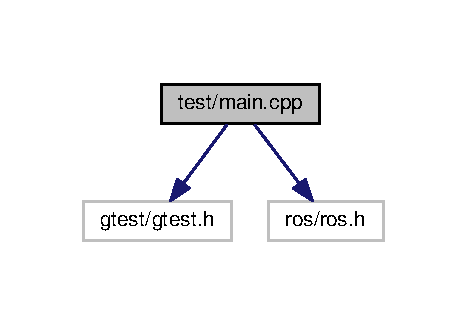
\includegraphics[width=224pt]{test_2main_8cpp__incl}
\end{center}
\end{figure}
\subsection*{Functions}
\begin{DoxyCompactItemize}
\item 
int \hyperlink{test_2main_8cpp_a3c04138a5bfe5d72780bb7e82a18e627}{main} (int argc, char $\ast$$\ast$argv)
\end{DoxyCompactItemize}


\subsection{Function Documentation}
\index{test/main.\+cpp@{test/main.\+cpp}!main@{main}}
\index{main@{main}!test/main.\+cpp@{test/main.\+cpp}}
\subsubsection[{\texorpdfstring{main(int argc, char $\ast$$\ast$argv)}{main(int argc, char **argv)}}]{\setlength{\rightskip}{0pt plus 5cm}int main (
\begin{DoxyParamCaption}
\item[{int}]{argc, }
\item[{char $\ast$$\ast$}]{argv}
\end{DoxyParamCaption}
)}\hypertarget{test_2main_8cpp_a3c04138a5bfe5d72780bb7e82a18e627}{}\label{test_2main_8cpp_a3c04138a5bfe5d72780bb7e82a18e627}


Definition at line 45 of file main.\+cpp.


\hypertarget{map_8cpp}{}\section{src/map.cpp File Reference}
\label{map_8cpp}\index{src/map.\+cpp@{src/map.\+cpp}}


To implementation of the class which implements the map.  


{\ttfamily \#include $<$ros/ros.\+h$>$}\\*
{\ttfamily \#include $<$nav\+\_\+msgs/\+Get\+Map.\+h$>$}\\*
{\ttfamily \#include $<$vector$>$}\\*
{\ttfamily \#include $<$queue$>$}\\*
{\ttfamily \#include $<$cmath$>$}\\*
{\ttfamily \#include \char`\"{}map.\+hpp\char`\"{}}\\*
{\ttfamily \#include \char`\"{}../include/\+B\+F\+S.\+hpp\char`\"{}}\\*
Include dependency graph for map.\+cpp\+:
\nopagebreak
\begin{figure}[H]
\begin{center}
\leavevmode
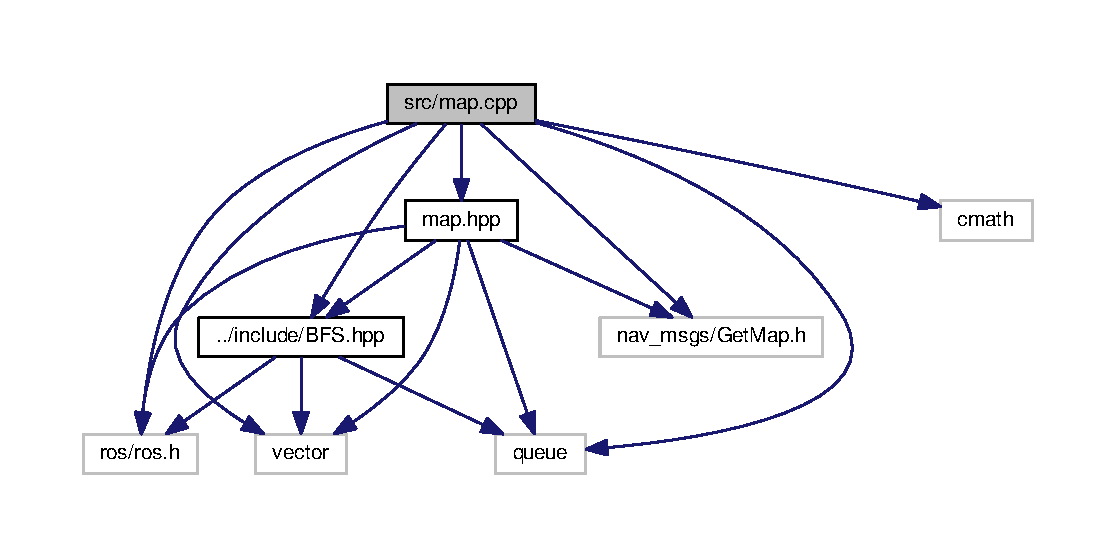
\includegraphics[width=350pt]{map_8cpp__incl}
\end{center}
\end{figure}


\subsection{Detailed Description}
To implementation of the class which implements the map. 

B\+SD 3-\/\+Clause License

Copyright (c) 2018, Nantha Kumar Sunder, Nithish Sanjeev Kumar All rights reserved.

Redistribution and use in source and binary forms, with or without modification, are permitted provided that the following conditions are met\+:


\begin{DoxyItemize}
\item Redistributions of source code must retain the above copyright notice, this list of conditions and the following disclaimer.
\item Redistributions in binary form must reproduce the above copyright notice, this list of conditions and the following disclaimer in the documentation and/or other materials provided with the distribution.
\item Neither the name of the copyright holder nor the names of its contributors may be used to endorse or promote products derived from this software without specific prior written permission.
\end{DoxyItemize}

T\+H\+IS S\+O\+F\+T\+W\+A\+RE IS P\+R\+O\+V\+I\+D\+ED BY T\+HE C\+O\+P\+Y\+R\+I\+G\+HT H\+O\+L\+D\+E\+RS A\+ND C\+O\+N\+T\+R\+I\+B\+U\+T\+O\+RS \char`\"{}\+A\+S I\+S\char`\"{} A\+ND A\+NY E\+X\+P\+R\+E\+SS OR I\+M\+P\+L\+I\+ED W\+A\+R\+R\+A\+N\+T\+I\+ES, I\+N\+C\+L\+U\+D\+I\+NG, B\+UT N\+OT L\+I\+M\+I\+T\+ED TO, T\+HE I\+M\+P\+L\+I\+ED W\+A\+R\+R\+A\+N\+T\+I\+ES OF M\+E\+R\+C\+H\+A\+N\+T\+A\+B\+I\+L\+I\+TY A\+ND F\+I\+T\+N\+E\+SS F\+OR A P\+A\+R\+T\+I\+C\+U\+L\+AR P\+U\+R\+P\+O\+SE A\+RE D\+I\+S\+C\+L\+A\+I\+M\+ED. IN NO E\+V\+E\+NT S\+H\+A\+LL T\+HE C\+O\+P\+Y\+R\+I\+G\+HT H\+O\+L\+D\+ER OR C\+O\+N\+T\+R\+I\+B\+U\+T\+O\+RS BE L\+I\+A\+B\+LE F\+OR A\+NY D\+I\+R\+E\+CT, I\+N\+D\+I\+R\+E\+CT, I\+N\+C\+I\+D\+E\+N\+T\+AL, S\+P\+E\+C\+I\+AL, E\+X\+E\+M\+P\+L\+A\+RY, OR C\+O\+N\+S\+E\+Q\+U\+E\+N\+T\+I\+AL D\+A\+M\+A\+G\+ES (I\+N\+C\+L\+U\+D\+I\+NG, B\+UT N\+OT L\+I\+M\+I\+T\+ED TO, P\+R\+O\+C\+U\+Rccen\+E\+M\+E\+NT OF S\+U\+B\+S\+T\+I\+T\+U\+TE G\+O\+O\+DS OR S\+E\+R\+V\+I\+C\+ES; L\+O\+SS OF U\+SE, D\+A\+TA, OR P\+R\+O\+F\+I\+TS; OR B\+U\+S\+I\+N\+E\+SS I\+N\+T\+E\+R\+R\+U\+P\+T\+I\+ON) H\+O\+W\+E\+V\+ER C\+A\+U\+S\+ED A\+ND ON A\+NY T\+H\+E\+O\+RY OF L\+I\+A\+B\+I\+L\+I\+TY, W\+H\+E\+T\+H\+ER IN C\+O\+N\+T\+R\+A\+CT, S\+T\+R\+I\+CT L\+I\+A\+B\+I\+L\+I\+TY, OR T\+O\+RT (I\+N\+C\+L\+U\+D\+I\+NG N\+E\+G\+L\+I\+G\+E\+N\+CE OR O\+T\+H\+E\+R\+W\+I\+SE) A\+R\+I\+S\+I\+NG IN A\+NY W\+AY O\+UT OF T\+HE U\+SE OF T\+H\+IS S\+O\+F\+T\+W\+A\+RE, E\+V\+EN IF A\+D\+V\+I\+S\+ED OF T\+HE P\+O\+S\+S\+I\+B\+I\+L\+I\+TY OF S\+U\+CH D\+A\+M\+A\+GE.

Nithish Sanjeev Kumar  Nantha Kumar Sunder \begin{DoxyCopyright}{Copyright}
2018 , Nantha Kumar Sunder, Nithish Sanjeev Kumar All rights reserved 
\end{DoxyCopyright}

\hypertarget{sensor_8cpp}{}\section{src/sensor.cpp File Reference}
\label{sensor_8cpp}\index{src/sensor.\+cpp@{src/sensor.\+cpp}}
{\ttfamily \#include $<$cmath$>$}\\*
{\ttfamily \#include $<$fstream$>$}\\*
{\ttfamily \#include $<$vector$>$}\\*
{\ttfamily \#include \char`\"{}../include/sensor.\+hpp\char`\"{}}\\*
Include dependency graph for sensor.\+cpp\+:
\nopagebreak
\begin{figure}[H]
\begin{center}
\leavevmode
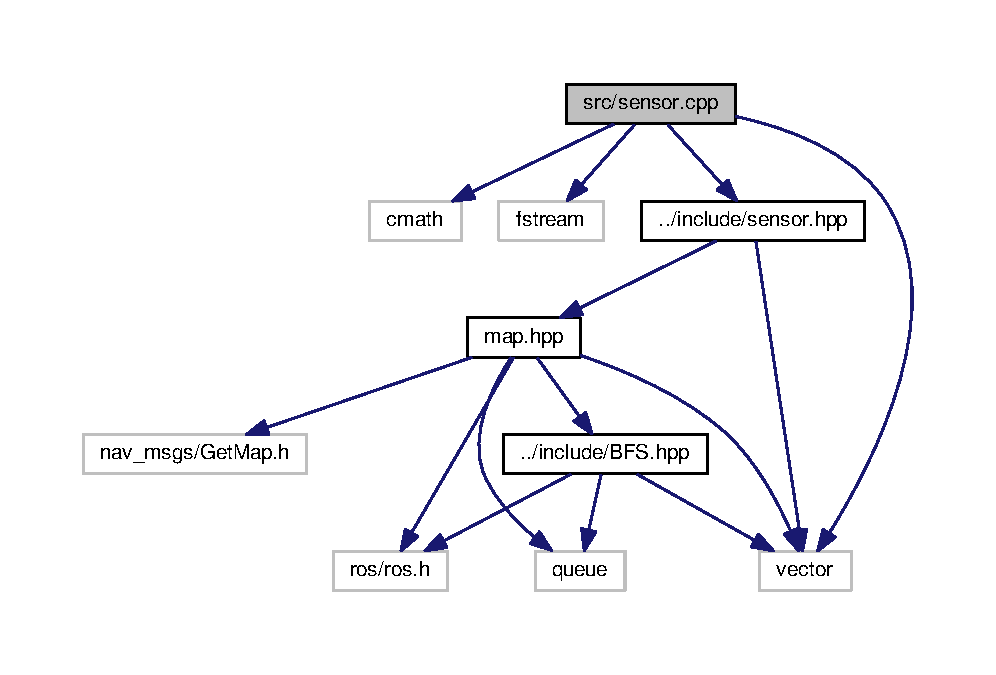
\includegraphics[width=350pt]{sensor_8cpp__incl}
\end{center}
\end{figure}

\hypertarget{testBFS_8cpp}{}\section{test/test\+B\+FS.cpp File Reference}
\label{testBFS_8cpp}\index{test/test\+B\+F\+S.\+cpp@{test/test\+B\+F\+S.\+cpp}}
{\ttfamily \#include $<$gtest/gtest.\+h$>$}\\*
{\ttfamily \#include $<$ros/ros.\+h$>$}\\*
{\ttfamily \#include $<$ros/service\+\_\+client.\+h$>$}\\*
{\ttfamily \#include $<$vector$>$}\\*
{\ttfamily \#include $<$queue$>$}\\*
{\ttfamily \#include \char`\"{}../include/\+B\+F\+S.\+hpp\char`\"{}}\\*
Include dependency graph for test\+B\+F\+S.\+cpp\+:
\nopagebreak
\begin{figure}[H]
\begin{center}
\leavevmode
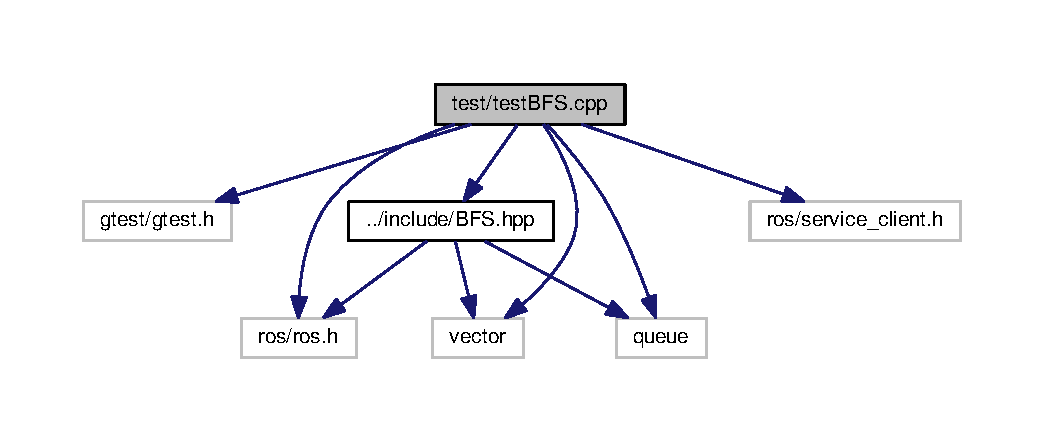
\includegraphics[width=350pt]{testBFS_8cpp__incl}
\end{center}
\end{figure}
\subsection*{Functions}
\begin{DoxyCompactItemize}
\item 
\hyperlink{testBFS_8cpp_ae04f729df8587db1f58afe0fa1d6a03f}{T\+E\+ST} (compute\+B\+FS, check\+B\+F\+S\+Alogrithm)
\item 
\hyperlink{testBFS_8cpp_af9df3b3b70f4af42aca089a716b075ab}{T\+E\+ST} (Neighbour\+List, check\+Neighbour\+List\+Output)
\item 
\hyperlink{testBFS_8cpp_a66a31bcb9df38b680336f9db921f588d}{T\+E\+ST} (get\+Explored, check\+Return\+Value)
\item 
\hyperlink{testBFS_8cpp_a704cc4b933a647cacc2f921bee19a211}{T\+E\+ST} (get\+Distance, check\+Return\+Value)
\end{DoxyCompactItemize}


\subsection{Function Documentation}
\index{test\+B\+F\+S.\+cpp@{test\+B\+F\+S.\+cpp}!T\+E\+ST@{T\+E\+ST}}
\index{T\+E\+ST@{T\+E\+ST}!test\+B\+F\+S.\+cpp@{test\+B\+F\+S.\+cpp}}
\subsubsection[{\texorpdfstring{T\+E\+S\+T(compute\+B\+F\+S, check\+B\+F\+S\+Alogrithm)}{TEST(computeBFS, checkBFSAlogrithm)}}]{\setlength{\rightskip}{0pt plus 5cm}T\+E\+ST (
\begin{DoxyParamCaption}
\item[{compute\+B\+FS}]{, }
\item[{check\+B\+F\+S\+Alogrithm}]{}
\end{DoxyParamCaption}
)}\hypertarget{testBFS_8cpp_ae04f729df8587db1f58afe0fa1d6a03f}{}\label{testBFS_8cpp_ae04f729df8587db1f58afe0fa1d6a03f}


Definition at line 49 of file test\+B\+F\+S.\+cpp.



References B\+F\+S\+::compute\+B\+F\+S().



Here is the call graph for this function\+:
\nopagebreak
\begin{figure}[H]
\begin{center}
\leavevmode
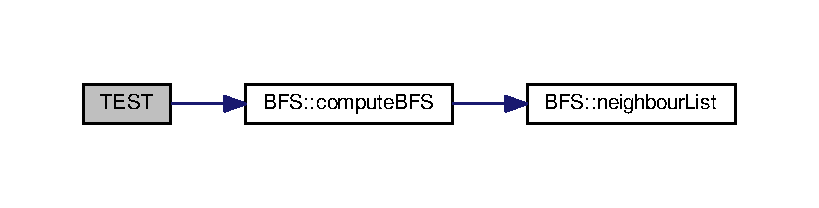
\includegraphics[width=350pt]{testBFS_8cpp_ae04f729df8587db1f58afe0fa1d6a03f_cgraph}
\end{center}
\end{figure}


\index{test\+B\+F\+S.\+cpp@{test\+B\+F\+S.\+cpp}!T\+E\+ST@{T\+E\+ST}}
\index{T\+E\+ST@{T\+E\+ST}!test\+B\+F\+S.\+cpp@{test\+B\+F\+S.\+cpp}}
\subsubsection[{\texorpdfstring{T\+E\+S\+T(\+Neighbour\+List, check\+Neighbour\+List\+Output)}{TEST(NeighbourList, checkNeighbourListOutput)}}]{\setlength{\rightskip}{0pt plus 5cm}T\+E\+ST (
\begin{DoxyParamCaption}
\item[{Neighbour\+List}]{, }
\item[{check\+Neighbour\+List\+Output}]{}
\end{DoxyParamCaption}
)}\hypertarget{testBFS_8cpp_af9df3b3b70f4af42aca089a716b075ab}{}\label{testBFS_8cpp_af9df3b3b70f4af42aca089a716b075ab}


Definition at line 80 of file test\+B\+F\+S.\+cpp.



References B\+F\+S\+::neighbour\+List().



Here is the call graph for this function\+:
\nopagebreak
\begin{figure}[H]
\begin{center}
\leavevmode
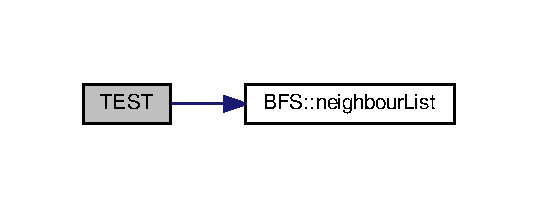
\includegraphics[width=258pt]{testBFS_8cpp_af9df3b3b70f4af42aca089a716b075ab_cgraph}
\end{center}
\end{figure}


\index{test\+B\+F\+S.\+cpp@{test\+B\+F\+S.\+cpp}!T\+E\+ST@{T\+E\+ST}}
\index{T\+E\+ST@{T\+E\+ST}!test\+B\+F\+S.\+cpp@{test\+B\+F\+S.\+cpp}}
\subsubsection[{\texorpdfstring{T\+E\+S\+T(get\+Explored, check\+Return\+Value)}{TEST(getExplored, checkReturnValue)}}]{\setlength{\rightskip}{0pt plus 5cm}T\+E\+ST (
\begin{DoxyParamCaption}
\item[{get\+Explored}]{, }
\item[{check\+Return\+Value}]{}
\end{DoxyParamCaption}
)}\hypertarget{testBFS_8cpp_a66a31bcb9df38b680336f9db921f588d}{}\label{testBFS_8cpp_a66a31bcb9df38b680336f9db921f588d}


Definition at line 114 of file test\+B\+F\+S.\+cpp.



References B\+F\+S\+::get\+Explored().



Here is the call graph for this function\+:
\nopagebreak
\begin{figure}[H]
\begin{center}
\leavevmode
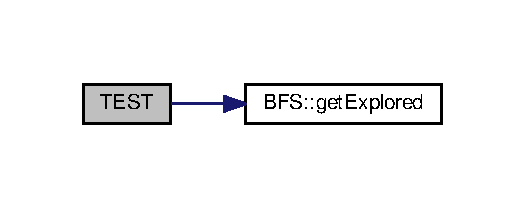
\includegraphics[width=252pt]{testBFS_8cpp_a66a31bcb9df38b680336f9db921f588d_cgraph}
\end{center}
\end{figure}


\index{test\+B\+F\+S.\+cpp@{test\+B\+F\+S.\+cpp}!T\+E\+ST@{T\+E\+ST}}
\index{T\+E\+ST@{T\+E\+ST}!test\+B\+F\+S.\+cpp@{test\+B\+F\+S.\+cpp}}
\subsubsection[{\texorpdfstring{T\+E\+S\+T(get\+Distance, check\+Return\+Value)}{TEST(getDistance, checkReturnValue)}}]{\setlength{\rightskip}{0pt plus 5cm}T\+E\+ST (
\begin{DoxyParamCaption}
\item[{get\+Distance}]{, }
\item[{check\+Return\+Value}]{}
\end{DoxyParamCaption}
)}\hypertarget{testBFS_8cpp_a704cc4b933a647cacc2f921bee19a211}{}\label{testBFS_8cpp_a704cc4b933a647cacc2f921bee19a211}


Definition at line 119 of file test\+B\+F\+S.\+cpp.



References B\+F\+S\+::get\+Distance().



Here is the call graph for this function\+:
\nopagebreak
\begin{figure}[H]
\begin{center}
\leavevmode
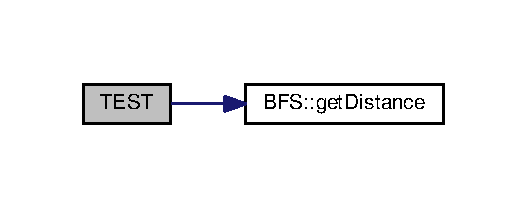
\includegraphics[width=253pt]{testBFS_8cpp_a704cc4b933a647cacc2f921bee19a211_cgraph}
\end{center}
\end{figure}



\hypertarget{testExplore_8cpp}{}\section{test/test\+Explore.cpp File Reference}
\label{testExplore_8cpp}\index{test/test\+Explore.\+cpp@{test/test\+Explore.\+cpp}}


To test the class explore.  


{\ttfamily \#include $<$gtest/gtest.\+h$>$}\\*
{\ttfamily \#include $<$ros/ros.\+h$>$}\\*
{\ttfamily \#include $<$vector$>$}\\*
{\ttfamily \#include $<$queue$>$}\\*
{\ttfamily \#include \char`\"{}map.\+hpp\char`\"{}}\\*
{\ttfamily \#include \char`\"{}explore.\+hpp\char`\"{}}\\*
Include dependency graph for test\+Explore.\+cpp\+:
\nopagebreak
\begin{figure}[H]
\begin{center}
\leavevmode
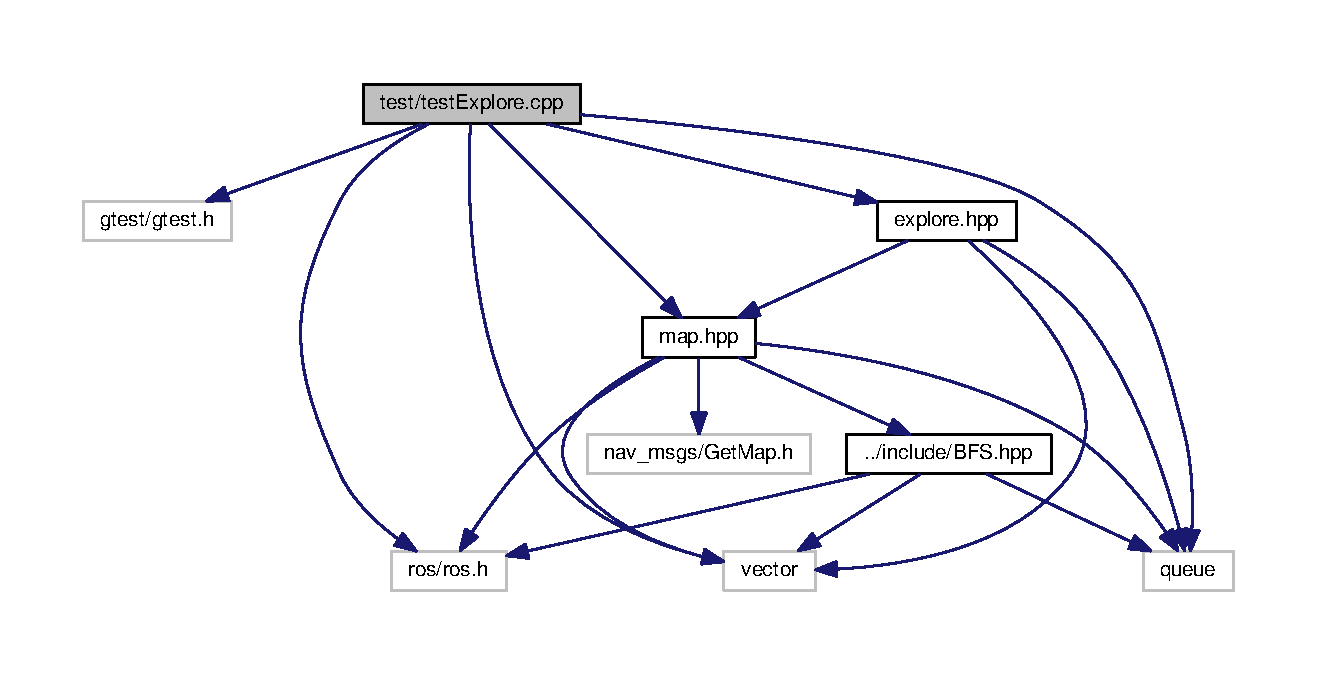
\includegraphics[width=350pt]{testExplore_8cpp__incl}
\end{center}
\end{figure}
\subsection*{Functions}
\begin{DoxyCompactItemize}
\item 
\hyperlink{testExplore_8cpp_afcc81a2b305ae7087ad05ab6b7fe8c3c}{T\+E\+ST} (find\+Obstacle\+Free\+Neighbours, To\+Find\+The\+Obtacle\+Free\+Neighbours)
\item 
\hyperlink{testExplore_8cpp_aaff8adb5fb0dfc1232a375f71faea03e}{T\+E\+ST} (compute\+Shortest\+Path, check\+Return\+Value)
\end{DoxyCompactItemize}


\subsection{Detailed Description}
To test the class explore. 

B\+SD 3-\/\+Clause License

Copyright (c) 2018, Nantha Kumar Sunder, Nithish Sanjeev Kumar All rights reserved.

Redistribution and use in source and binary forms, with or without modification, are permitted provided that the following conditions are met\+:


\begin{DoxyItemize}
\item Redistributions of source code must retain the above copyright notice, this list of conditions and the following disclaimer.
\item Redistributions in binary form must reproduce the above copyright notice, this list of conditions and the following disclaimer in the documentation and/or other materials provided with the distribution.
\item Neither the name of the copyright holder nor the names of its contributors may be used to endorse or promote products derived from this software without specific prior written permission.
\end{DoxyItemize}

T\+H\+IS S\+O\+F\+T\+W\+A\+RE IS P\+R\+O\+V\+I\+D\+ED BY T\+HE C\+O\+P\+Y\+R\+I\+G\+HT H\+O\+L\+D\+E\+RS A\+ND C\+O\+N\+T\+R\+I\+B\+U\+T\+O\+RS \char`\"{}\+A\+S I\+S\char`\"{} A\+ND A\+NY E\+X\+P\+R\+E\+SS OR I\+M\+P\+L\+I\+ED W\+A\+R\+R\+A\+N\+T\+I\+ES, I\+N\+C\+L\+U\+D\+I\+NG, B\+UT N\+OT L\+I\+M\+I\+T\+ED TO, T\+HE I\+M\+P\+L\+I\+ED W\+A\+R\+R\+A\+N\+T\+I\+ES OF M\+E\+R\+C\+H\+A\+N\+T\+A\+B\+I\+L\+I\+TY A\+ND F\+I\+T\+N\+E\+SS F\+OR A P\+A\+R\+T\+I\+C\+U\+L\+AR P\+U\+R\+P\+O\+SE A\+RE D\+I\+S\+C\+L\+A\+I\+M\+ED. IN NO E\+V\+E\+NT S\+H\+A\+LL T\+HE C\+O\+P\+Y\+R\+I\+G\+HT H\+O\+L\+D\+ER OR C\+O\+N\+T\+R\+I\+B\+U\+T\+O\+RS BE L\+I\+A\+B\+LE F\+OR A\+NY D\+I\+R\+E\+CT, I\+N\+D\+I\+R\+E\+CT, I\+N\+C\+I\+D\+E\+N\+T\+AL, S\+P\+E\+C\+I\+AL, E\+X\+E\+M\+P\+L\+A\+RY, OR C\+O\+N\+S\+E\+Q\+U\+E\+N\+T\+I\+AL D\+A\+M\+A\+G\+ES (I\+N\+C\+L\+U\+D\+I\+NG, B\+UT N\+OT L\+I\+M\+I\+T\+ED TO, P\+R\+O\+C\+U\+R\+E\+M\+E\+NT OF S\+U\+B\+S\+T\+I\+T\+U\+TE G\+O\+O\+DS OR S\+E\+R\+V\+I\+C\+ES; L\+O\+SS OF U\+SE, D\+A\+TA, OR P\+R\+O\+F\+I\+TS; OR B\+U\+S\+I\+N\+E\+SS I\+N\+T\+E\+R\+R\+U\+P\+T\+I\+ON) H\+O\+W\+E\+V\+ER C\+A\+U\+S\+ED A\+ND ON A\+NY T\+H\+E\+O\+RY OF L\+I\+A\+B\+I\+L\+I\+TY, W\+H\+E\+T\+H\+ER IN C\+O\+N\+T\+R\+A\+CT, S\+T\+R\+I\+CT L\+I\+A\+B\+I\+L\+I\+TY, OR T\+O\+RT (I\+N\+C\+L\+U\+D\+I\+NG N\+E\+G\+L\+I\+G\+E\+N\+CE OR O\+T\+H\+E\+R\+W\+I\+SE) A\+R\+I\+S\+I\+NG IN A\+NY W\+AY O\+UT OF T\+HE U\+SE OF T\+H\+IS S\+O\+F\+T\+W\+A\+RE, E\+V\+EN IF A\+D\+V\+I\+S\+ED OF T\+HE P\+O\+S\+S\+I\+B\+I\+L\+I\+TY OF S\+U\+CH D\+A\+M\+A\+GE.

Nithish Sanjeev Kumar  Nantha Kumar Sunder \begin{DoxyCopyright}{Copyright}
2018 , Nantha Kumar Sunder, Nithish Sanjeev Kumar All rights reserved 
\end{DoxyCopyright}


\subsection{Function Documentation}
\index{test\+Explore.\+cpp@{test\+Explore.\+cpp}!T\+E\+ST@{T\+E\+ST}}
\index{T\+E\+ST@{T\+E\+ST}!test\+Explore.\+cpp@{test\+Explore.\+cpp}}
\subsubsection[{\texorpdfstring{T\+E\+S\+T(find\+Obstacle\+Free\+Neighbours, To\+Find\+The\+Obtacle\+Free\+Neighbours)}{TEST(findObstacleFreeNeighbours, ToFindTheObtacleFreeNeighbours)}}]{\setlength{\rightskip}{0pt plus 5cm}T\+E\+ST (
\begin{DoxyParamCaption}
\item[{find\+Obstacle\+Free\+Neighbours}]{, }
\item[{To\+Find\+The\+Obtacle\+Free\+Neighbours}]{}
\end{DoxyParamCaption}
)}\hypertarget{testExplore_8cpp_afcc81a2b305ae7087ad05ab6b7fe8c3c}{}\label{testExplore_8cpp_afcc81a2b305ae7087ad05ab6b7fe8c3c}


Definition at line 49 of file test\+Explore.\+cpp.



References explore\+::find\+Obstacle\+Free\+Neighbours().



Here is the call graph for this function\+:
\nopagebreak
\begin{figure}[H]
\begin{center}
\leavevmode
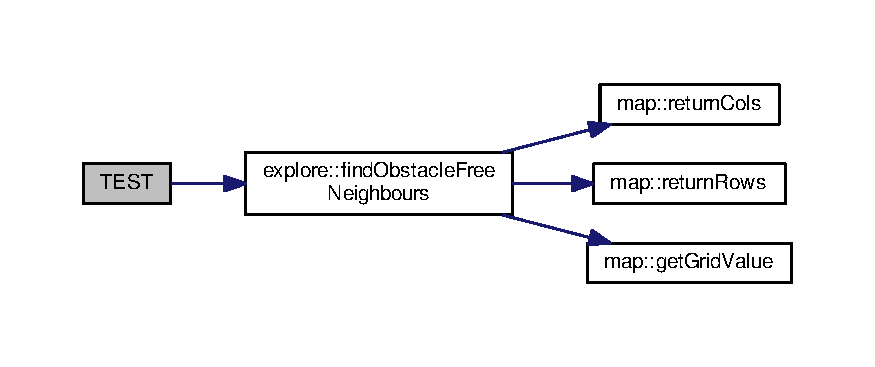
\includegraphics[width=350pt]{testExplore_8cpp_afcc81a2b305ae7087ad05ab6b7fe8c3c_cgraph}
\end{center}
\end{figure}


\index{test\+Explore.\+cpp@{test\+Explore.\+cpp}!T\+E\+ST@{T\+E\+ST}}
\index{T\+E\+ST@{T\+E\+ST}!test\+Explore.\+cpp@{test\+Explore.\+cpp}}
\subsubsection[{\texorpdfstring{T\+E\+S\+T(compute\+Shortest\+Path, check\+Return\+Value)}{TEST(computeShortestPath, checkReturnValue)}}]{\setlength{\rightskip}{0pt plus 5cm}T\+E\+ST (
\begin{DoxyParamCaption}
\item[{compute\+Shortest\+Path}]{, }
\item[{check\+Return\+Value}]{}
\end{DoxyParamCaption}
)}\hypertarget{testExplore_8cpp_aaff8adb5fb0dfc1232a375f71faea03e}{}\label{testExplore_8cpp_aaff8adb5fb0dfc1232a375f71faea03e}


Definition at line 65 of file test\+Explore.\+cpp.



References explore\+::compute\+Shortest\+Path().



Here is the call graph for this function\+:
\nopagebreak
\begin{figure}[H]
\begin{center}
\leavevmode
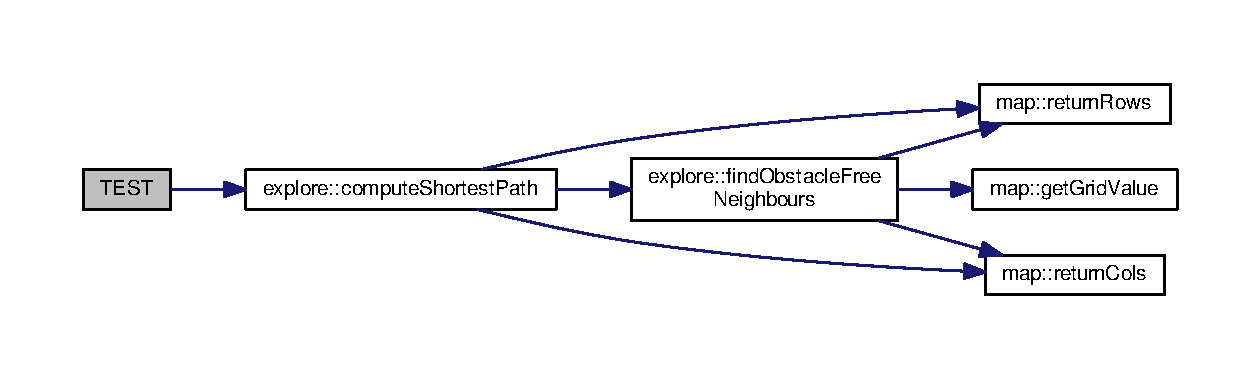
\includegraphics[width=350pt]{testExplore_8cpp_aaff8adb5fb0dfc1232a375f71faea03e_cgraph}
\end{center}
\end{figure}



\hypertarget{testMapGen_8cpp}{}\section{test/test\+Map\+Gen.cpp File Reference}
\label{testMapGen_8cpp}\index{test/test\+Map\+Gen.\+cpp@{test/test\+Map\+Gen.\+cpp}}


To test the class map\+Gen.  


{\ttfamily \#include $<$gtest/gtest.\+h$>$}\\*
{\ttfamily \#include $<$ros/ros.\+h$>$}\\*
{\ttfamily \#include $<$ros/service\+\_\+client.\+h$>$}\\*
{\ttfamily \#include \char`\"{}map.\+hpp\char`\"{}}\\*
{\ttfamily \#include \char`\"{}B\+F\+S.\+hpp\char`\"{}}\\*
Include dependency graph for test\+Map\+Gen.\+cpp\+:
\nopagebreak
\begin{figure}[H]
\begin{center}
\leavevmode
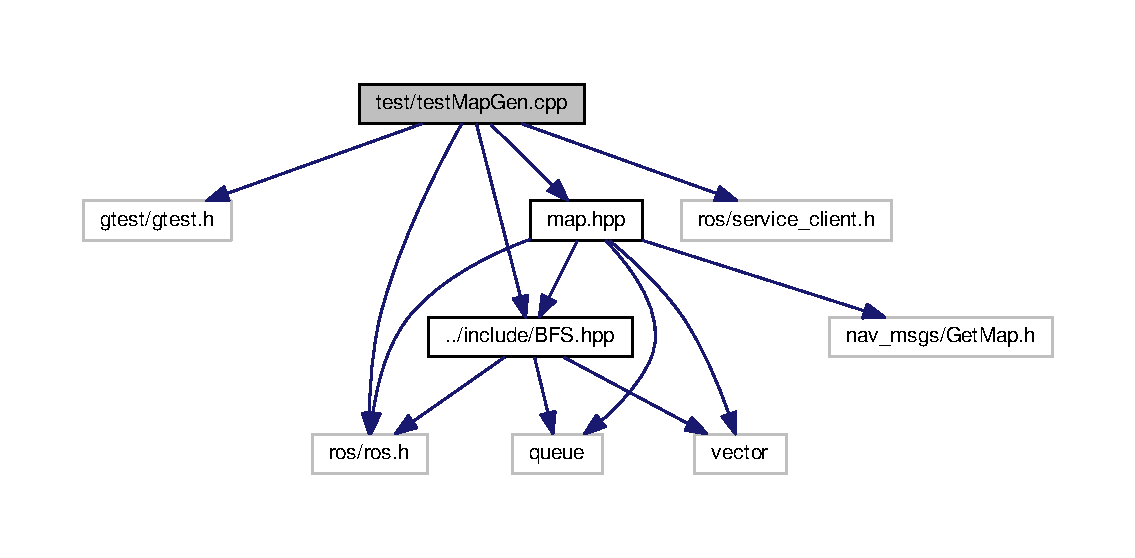
\includegraphics[width=350pt]{testMapGen_8cpp__incl}
\end{center}
\end{figure}
\subsection*{Functions}
\begin{DoxyCompactItemize}
\item 
\hyperlink{testMapGen_8cpp_a2092d45a9092550679406ae44957256c}{T\+E\+ST} (request\+Map, check\+Node\+Activation)
\item 
\hyperlink{testMapGen_8cpp_a82f7b5240c76a845f836dcf397e3cd38}{T\+E\+ST} (frontier\+Search, Check\+Frontier\+Search)
\item 
\hyperlink{testMapGen_8cpp_a71b9bb9521f3381729de7e198fc5ab07}{T\+E\+ST} (check\+Neighbour, Check\+Frontier\+Search)
\item 
\hyperlink{testMapGen_8cpp_adbb3cfc7b0c1e61d71ed72aa84f8ae90}{T\+E\+ST} (Get\+Resolution, Check\+Resolution)
\item 
\hyperlink{testMapGen_8cpp_a9de61f4534bff97afed629b7543f97ed}{T\+E\+ST} (nearest, check\+Return\+Value)
\item 
\hyperlink{testMapGen_8cpp_a74230d688d2a3a1bf058aa97bb0760dd}{T\+E\+ST} (compute\+Frontier\+Centroid, check\+Centroid\+Value)
\item 
\hyperlink{testMapGen_8cpp_a262fd421e6225192e2ab37f27334a59b}{T\+E\+ST} (Return\+Rows, check\+Return\+Value\+Of\+Row)
\item 
\hyperlink{testMapGen_8cpp_ae9436b25d0925fbbbff0264319898b61}{T\+E\+ST} (Return\+Cols, check\+Return\+Value\+Of\+Cols)
\item 
\hyperlink{testMapGen_8cpp_a225a868ba83e0d799c6358d626ad76cd}{T\+E\+ST} (Get\+Grid\+Value, check\+Get\+Grid\+Value)
\end{DoxyCompactItemize}


\subsection{Detailed Description}
To test the class map\+Gen. 

B\+SD 3-\/\+Clause License

Copyright (c) 2018, Nantha Kumar Sunder, Nithish Sanjeev Kumar All rights reserved.

Redistribution and use in source and binary forms, with or without modification, are permitted provided that the following conditions are met\+:


\begin{DoxyItemize}
\item Redistributions of source code must retain the above copyright notice, this list of conditions and the following disclaimer.
\item Redistributions in binary form must reproduce the above copyright notice, this list of conditions and the following disclaimer in the documentation and/or other materials provided with the distribution.
\item Neither the name of the copyright holder nor the names of its contributors may be used to endorse or promote products derived from this software without specific prior written permission.
\end{DoxyItemize}

T\+H\+IS S\+O\+F\+T\+W\+A\+RE IS P\+R\+O\+V\+I\+D\+ED BY T\+HE C\+O\+P\+Y\+R\+I\+G\+HT H\+O\+L\+D\+E\+RS A\+ND C\+O\+N\+T\+R\+I\+B\+U\+T\+O\+RS \char`\"{}\+A\+S I\+S\char`\"{} A\+ND A\+NY E\+X\+P\+R\+E\+SS OR I\+M\+P\+L\+I\+ED W\+A\+R\+R\+A\+N\+T\+I\+ES, I\+N\+C\+L\+U\+D\+I\+NG, B\+UT N\+OT L\+I\+M\+I\+T\+ED TO, T\+HE I\+M\+P\+L\+I\+ED W\+A\+R\+R\+A\+N\+T\+I\+ES OF M\+E\+R\+C\+H\+A\+N\+T\+A\+B\+I\+L\+I\+TY A\+ND F\+I\+T\+N\+E\+SS F\+OR A P\+A\+R\+T\+I\+C\+U\+L\+AR P\+U\+R\+P\+O\+SE A\+RE D\+I\+S\+C\+L\+A\+I\+M\+ED. IN NO E\+V\+E\+NT S\+H\+A\+LL T\+HE C\+O\+P\+Y\+R\+I\+G\+HT H\+O\+L\+D\+ER OR C\+O\+N\+T\+R\+I\+B\+U\+T\+O\+RS BE L\+I\+A\+B\+LE F\+OR A\+NY D\+I\+R\+E\+CT, I\+N\+D\+I\+R\+E\+CT, I\+N\+C\+I\+D\+E\+N\+T\+AL, S\+P\+E\+C\+I\+AL, E\+X\+E\+M\+P\+L\+A\+RY, OR C\+O\+N\+S\+E\+Q\+U\+E\+N\+T\+I\+AL D\+A\+M\+A\+G\+ES (I\+N\+C\+L\+U\+D\+I\+NG, B\+UT N\+OT L\+I\+M\+I\+T\+ED TO, P\+R\+O\+C\+U\+R\+E\+M\+E\+NT OF S\+U\+B\+S\+T\+I\+T\+U\+TE G\+O\+O\+DS OR S\+E\+R\+V\+I\+C\+ES; L\+O\+SS OF U\+SE, D\+A\+TA, OR P\+R\+O\+F\+I\+TS; OR B\+U\+S\+I\+N\+E\+SS I\+N\+T\+E\+R\+R\+U\+P\+T\+I\+ON) H\+O\+W\+E\+V\+ER C\+A\+U\+S\+ED A\+ND ON A\+NY T\+H\+E\+O\+RY OF L\+I\+A\+B\+I\+L\+I\+TY, W\+H\+E\+T\+H\+ER IN C\+O\+N\+T\+R\+A\+CT, S\+T\+R\+I\+CT L\+I\+A\+B\+I\+L\+I\+TY, OR T\+O\+RT (I\+N\+C\+L\+U\+D\+I\+NG N\+E\+G\+L\+I\+G\+E\+N\+CE OR O\+T\+H\+E\+R\+W\+I\+SE) A\+R\+I\+S\+I\+NG IN A\+NY W\+AY O\+UT OF T\+HE U\+SE OF T\+H\+IS S\+O\+F\+T\+W\+A\+RE, E\+V\+EN IF A\+D\+V\+I\+S\+ED OF T\+HE P\+O\+S\+S\+I\+B\+I\+L\+I\+TY OF S\+U\+CH D\+A\+M\+A\+GE.

Nithish Sanjeev Kumar  Nantha Kumar Sunder \begin{DoxyCopyright}{Copyright}
2018 , Nantha Kumar Sunder, Nithish Sanjeev Kumar All rights reserved 
\end{DoxyCopyright}


\subsection{Function Documentation}
\index{test\+Map\+Gen.\+cpp@{test\+Map\+Gen.\+cpp}!T\+E\+ST@{T\+E\+ST}}
\index{T\+E\+ST@{T\+E\+ST}!test\+Map\+Gen.\+cpp@{test\+Map\+Gen.\+cpp}}
\subsubsection[{\texorpdfstring{T\+E\+S\+T(request\+Map, check\+Node\+Activation)}{TEST(requestMap, checkNodeActivation)}}]{\setlength{\rightskip}{0pt plus 5cm}T\+E\+ST (
\begin{DoxyParamCaption}
\item[{request\+Map}]{, }
\item[{check\+Node\+Activation}]{}
\end{DoxyParamCaption}
)}\hypertarget{testMapGen_8cpp_a2092d45a9092550679406ae44957256c}{}\label{testMapGen_8cpp_a2092d45a9092550679406ae44957256c}


Definition at line 49 of file test\+Map\+Gen.\+cpp.



References map\+::request\+Map().



Here is the call graph for this function\+:
\nopagebreak
\begin{figure}[H]
\begin{center}
\leavevmode
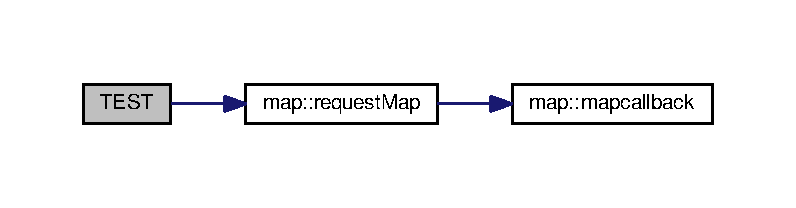
\includegraphics[width=350pt]{testMapGen_8cpp_a2092d45a9092550679406ae44957256c_cgraph}
\end{center}
\end{figure}


\index{test\+Map\+Gen.\+cpp@{test\+Map\+Gen.\+cpp}!T\+E\+ST@{T\+E\+ST}}
\index{T\+E\+ST@{T\+E\+ST}!test\+Map\+Gen.\+cpp@{test\+Map\+Gen.\+cpp}}
\subsubsection[{\texorpdfstring{T\+E\+S\+T(frontier\+Search, Check\+Frontier\+Search)}{TEST(frontierSearch, CheckFrontierSearch)}}]{\setlength{\rightskip}{0pt plus 5cm}T\+E\+ST (
\begin{DoxyParamCaption}
\item[{frontier\+Search}]{, }
\item[{Check\+Frontier\+Search}]{}
\end{DoxyParamCaption}
)}\hypertarget{testMapGen_8cpp_a82f7b5240c76a845f836dcf397e3cd38}{}\label{testMapGen_8cpp_a82f7b5240c76a845f836dcf397e3cd38}


Definition at line 64 of file test\+Map\+Gen.\+cpp.



References map\+::frontier\+Search(), and map\+::get\+Centroid\+Size().



Here is the call graph for this function\+:
\nopagebreak
\begin{figure}[H]
\begin{center}
\leavevmode
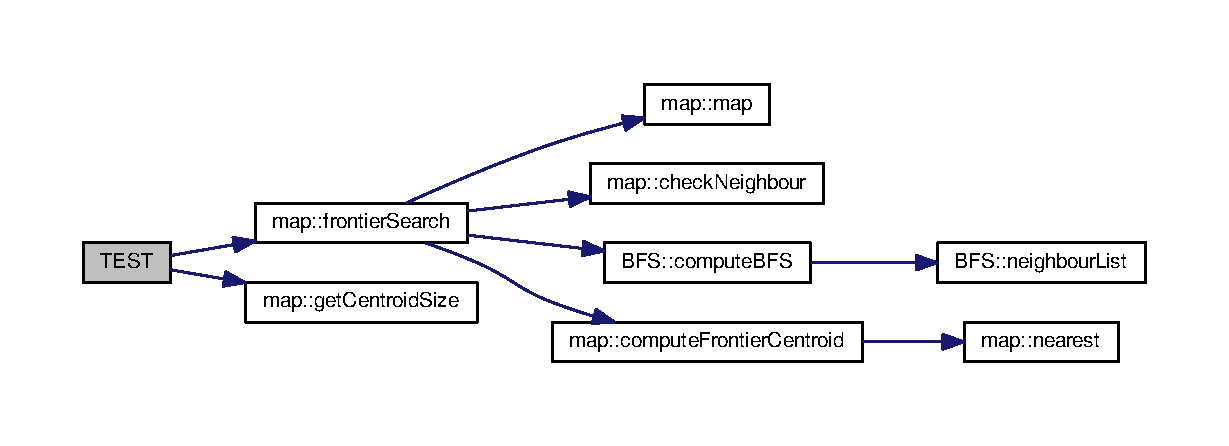
\includegraphics[width=350pt]{testMapGen_8cpp_a82f7b5240c76a845f836dcf397e3cd38_cgraph}
\end{center}
\end{figure}


\index{test\+Map\+Gen.\+cpp@{test\+Map\+Gen.\+cpp}!T\+E\+ST@{T\+E\+ST}}
\index{T\+E\+ST@{T\+E\+ST}!test\+Map\+Gen.\+cpp@{test\+Map\+Gen.\+cpp}}
\subsubsection[{\texorpdfstring{T\+E\+S\+T(check\+Neighbour, Check\+Frontier\+Search)}{TEST(checkNeighbour, CheckFrontierSearch)}}]{\setlength{\rightskip}{0pt plus 5cm}T\+E\+ST (
\begin{DoxyParamCaption}
\item[{check\+Neighbour}]{, }
\item[{Check\+Frontier\+Search}]{}
\end{DoxyParamCaption}
)}\hypertarget{testMapGen_8cpp_a71b9bb9521f3381729de7e198fc5ab07}{}\label{testMapGen_8cpp_a71b9bb9521f3381729de7e198fc5ab07}


Definition at line 74 of file test\+Map\+Gen.\+cpp.



References map\+::check\+Neighbour().



Here is the call graph for this function\+:
\nopagebreak
\begin{figure}[H]
\begin{center}
\leavevmode
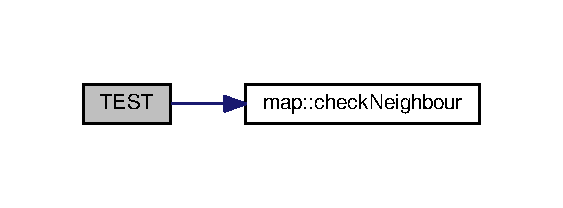
\includegraphics[width=270pt]{testMapGen_8cpp_a71b9bb9521f3381729de7e198fc5ab07_cgraph}
\end{center}
\end{figure}


\index{test\+Map\+Gen.\+cpp@{test\+Map\+Gen.\+cpp}!T\+E\+ST@{T\+E\+ST}}
\index{T\+E\+ST@{T\+E\+ST}!test\+Map\+Gen.\+cpp@{test\+Map\+Gen.\+cpp}}
\subsubsection[{\texorpdfstring{T\+E\+S\+T(\+Get\+Resolution, Check\+Resolution)}{TEST(GetResolution, CheckResolution)}}]{\setlength{\rightskip}{0pt plus 5cm}T\+E\+ST (
\begin{DoxyParamCaption}
\item[{Get\+Resolution}]{, }
\item[{Check\+Resolution}]{}
\end{DoxyParamCaption}
)}\hypertarget{testMapGen_8cpp_adbb3cfc7b0c1e61d71ed72aa84f8ae90}{}\label{testMapGen_8cpp_adbb3cfc7b0c1e61d71ed72aa84f8ae90}


Definition at line 79 of file test\+Map\+Gen.\+cpp.



References map\+::get\+Resolution().



Here is the call graph for this function\+:
\nopagebreak
\begin{figure}[H]
\begin{center}
\leavevmode
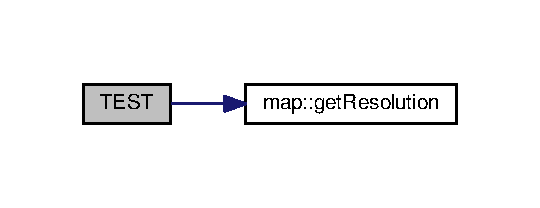
\includegraphics[width=259pt]{testMapGen_8cpp_adbb3cfc7b0c1e61d71ed72aa84f8ae90_cgraph}
\end{center}
\end{figure}


\index{test\+Map\+Gen.\+cpp@{test\+Map\+Gen.\+cpp}!T\+E\+ST@{T\+E\+ST}}
\index{T\+E\+ST@{T\+E\+ST}!test\+Map\+Gen.\+cpp@{test\+Map\+Gen.\+cpp}}
\subsubsection[{\texorpdfstring{T\+E\+S\+T(nearest, check\+Return\+Value)}{TEST(nearest, checkReturnValue)}}]{\setlength{\rightskip}{0pt plus 5cm}T\+E\+ST (
\begin{DoxyParamCaption}
\item[{nearest}]{, }
\item[{check\+Return\+Value}]{}
\end{DoxyParamCaption}
)}\hypertarget{testMapGen_8cpp_a9de61f4534bff97afed629b7543f97ed}{}\label{testMapGen_8cpp_a9de61f4534bff97afed629b7543f97ed}


Definition at line 84 of file test\+Map\+Gen.\+cpp.



References map\+::nearest().



Here is the call graph for this function\+:
\nopagebreak
\begin{figure}[H]
\begin{center}
\leavevmode
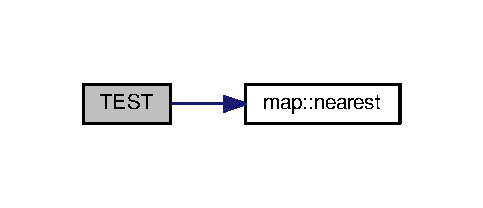
\includegraphics[width=232pt]{testMapGen_8cpp_a9de61f4534bff97afed629b7543f97ed_cgraph}
\end{center}
\end{figure}


\index{test\+Map\+Gen.\+cpp@{test\+Map\+Gen.\+cpp}!T\+E\+ST@{T\+E\+ST}}
\index{T\+E\+ST@{T\+E\+ST}!test\+Map\+Gen.\+cpp@{test\+Map\+Gen.\+cpp}}
\subsubsection[{\texorpdfstring{T\+E\+S\+T(compute\+Frontier\+Centroid, check\+Centroid\+Value)}{TEST(computeFrontierCentroid, checkCentroidValue)}}]{\setlength{\rightskip}{0pt plus 5cm}T\+E\+ST (
\begin{DoxyParamCaption}
\item[{compute\+Frontier\+Centroid}]{, }
\item[{check\+Centroid\+Value}]{}
\end{DoxyParamCaption}
)}\hypertarget{testMapGen_8cpp_a74230d688d2a3a1bf058aa97bb0760dd}{}\label{testMapGen_8cpp_a74230d688d2a3a1bf058aa97bb0760dd}


Definition at line 110 of file test\+Map\+Gen.\+cpp.



References map\+::compute\+Frontier\+Centroid().



Here is the call graph for this function\+:
\nopagebreak
\begin{figure}[H]
\begin{center}
\leavevmode
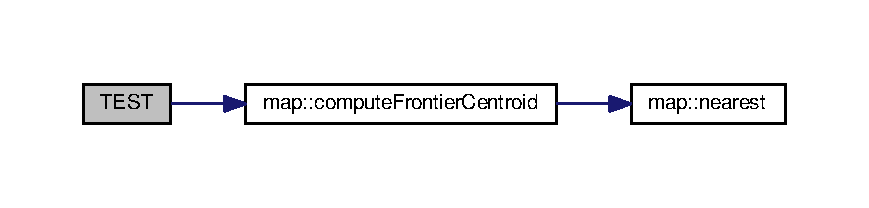
\includegraphics[width=350pt]{testMapGen_8cpp_a74230d688d2a3a1bf058aa97bb0760dd_cgraph}
\end{center}
\end{figure}


\index{test\+Map\+Gen.\+cpp@{test\+Map\+Gen.\+cpp}!T\+E\+ST@{T\+E\+ST}}
\index{T\+E\+ST@{T\+E\+ST}!test\+Map\+Gen.\+cpp@{test\+Map\+Gen.\+cpp}}
\subsubsection[{\texorpdfstring{T\+E\+S\+T(\+Return\+Rows, check\+Return\+Value\+Of\+Row)}{TEST(ReturnRows, checkReturnValueOfRow)}}]{\setlength{\rightskip}{0pt plus 5cm}T\+E\+ST (
\begin{DoxyParamCaption}
\item[{Return\+Rows}]{, }
\item[{check\+Return\+Value\+Of\+Row}]{}
\end{DoxyParamCaption}
)}\hypertarget{testMapGen_8cpp_a262fd421e6225192e2ab37f27334a59b}{}\label{testMapGen_8cpp_a262fd421e6225192e2ab37f27334a59b}


Definition at line 134 of file test\+Map\+Gen.\+cpp.



References map\+::return\+Rows().



Here is the call graph for this function\+:
\nopagebreak
\begin{figure}[H]
\begin{center}
\leavevmode
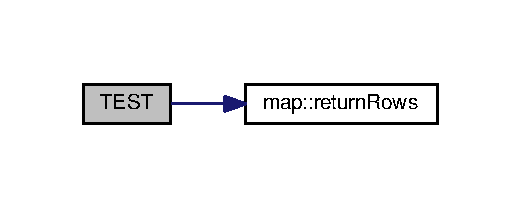
\includegraphics[width=250pt]{testMapGen_8cpp_a262fd421e6225192e2ab37f27334a59b_cgraph}
\end{center}
\end{figure}


\index{test\+Map\+Gen.\+cpp@{test\+Map\+Gen.\+cpp}!T\+E\+ST@{T\+E\+ST}}
\index{T\+E\+ST@{T\+E\+ST}!test\+Map\+Gen.\+cpp@{test\+Map\+Gen.\+cpp}}
\subsubsection[{\texorpdfstring{T\+E\+S\+T(\+Return\+Cols, check\+Return\+Value\+Of\+Cols)}{TEST(ReturnCols, checkReturnValueOfCols)}}]{\setlength{\rightskip}{0pt plus 5cm}T\+E\+ST (
\begin{DoxyParamCaption}
\item[{Return\+Cols}]{, }
\item[{check\+Return\+Value\+Of\+Cols}]{}
\end{DoxyParamCaption}
)}\hypertarget{testMapGen_8cpp_ae9436b25d0925fbbbff0264319898b61}{}\label{testMapGen_8cpp_ae9436b25d0925fbbbff0264319898b61}


Definition at line 138 of file test\+Map\+Gen.\+cpp.



References map\+::return\+Cols().



Here is the call graph for this function\+:
\nopagebreak
\begin{figure}[H]
\begin{center}
\leavevmode
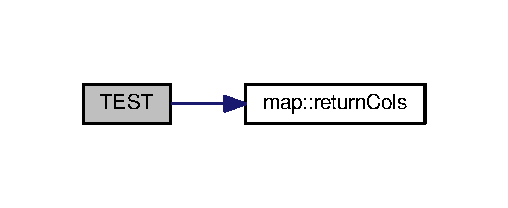
\includegraphics[width=244pt]{testMapGen_8cpp_ae9436b25d0925fbbbff0264319898b61_cgraph}
\end{center}
\end{figure}


\index{test\+Map\+Gen.\+cpp@{test\+Map\+Gen.\+cpp}!T\+E\+ST@{T\+E\+ST}}
\index{T\+E\+ST@{T\+E\+ST}!test\+Map\+Gen.\+cpp@{test\+Map\+Gen.\+cpp}}
\subsubsection[{\texorpdfstring{T\+E\+S\+T(\+Get\+Grid\+Value, check\+Get\+Grid\+Value)}{TEST(GetGridValue, checkGetGridValue)}}]{\setlength{\rightskip}{0pt plus 5cm}T\+E\+ST (
\begin{DoxyParamCaption}
\item[{Get\+Grid\+Value}]{, }
\item[{check\+Get\+Grid\+Value}]{}
\end{DoxyParamCaption}
)}\hypertarget{testMapGen_8cpp_a225a868ba83e0d799c6358d626ad76cd}{}\label{testMapGen_8cpp_a225a868ba83e0d799c6358d626ad76cd}


Definition at line 142 of file test\+Map\+Gen.\+cpp.



References map\+::get\+Grid\+Value().



Here is the call graph for this function\+:
\nopagebreak
\begin{figure}[H]
\begin{center}
\leavevmode
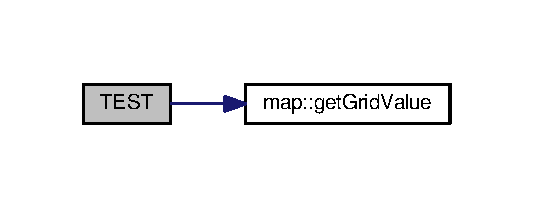
\includegraphics[width=256pt]{testMapGen_8cpp_a225a868ba83e0d799c6358d626ad76cd_cgraph}
\end{center}
\end{figure}



\hypertarget{testSensor_8cpp}{}\section{test/test\+Sensor.cpp File Reference}
\label{testSensor_8cpp}\index{test/test\+Sensor.\+cpp@{test/test\+Sensor.\+cpp}}


To test the class sensor.  


{\ttfamily \#include $<$gtest/gtest.\+h$>$}\\*
{\ttfamily \#include $<$ros/ros.\+h$>$}\\*
{\ttfamily \#include $<$ros/service\+\_\+client.\+h$>$}\\*
{\ttfamily \#include \char`\"{}map.\+hpp\char`\"{}}\\*
{\ttfamily \#include \char`\"{}B\+F\+S.\+hpp\char`\"{}}\\*
{\ttfamily \#include \char`\"{}sensor.\+hpp\char`\"{}}\\*
Include dependency graph for test\+Sensor.\+cpp\+:
\nopagebreak
\begin{figure}[H]
\begin{center}
\leavevmode
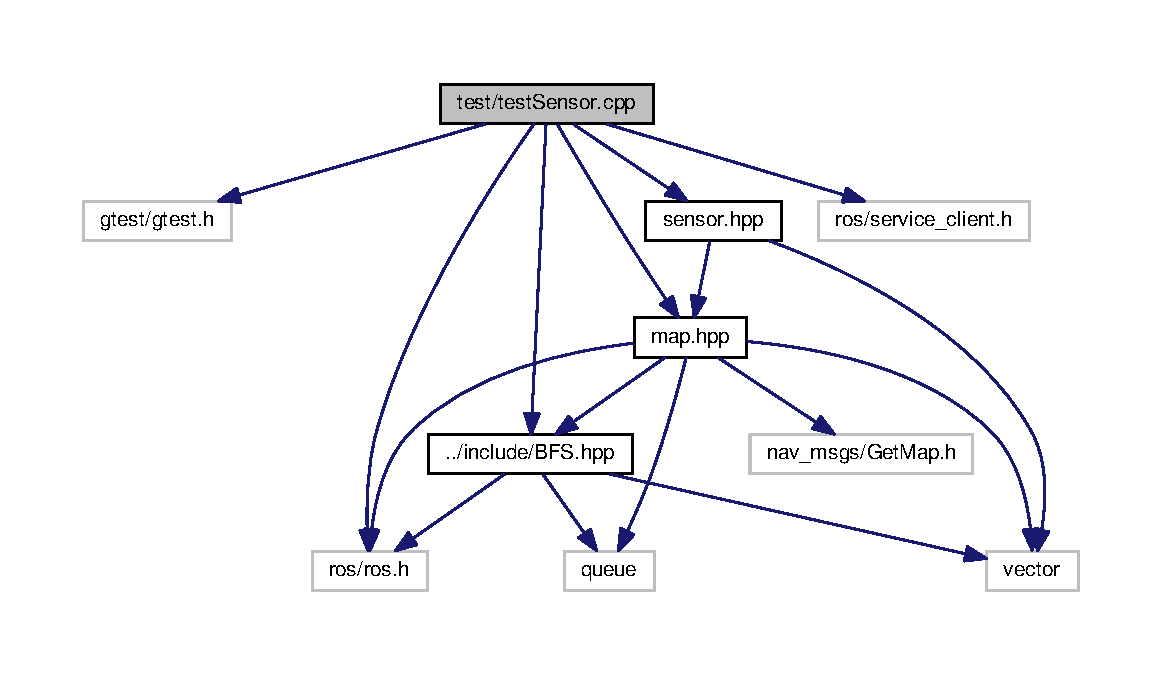
\includegraphics[width=350pt]{testSensor_8cpp__incl}
\end{center}
\end{figure}
\subsection*{Functions}
\begin{DoxyCompactItemize}
\item 
\hyperlink{testSensor_8cpp_acde73c74a87cd4e2a6be903ae254b3ae}{T\+E\+ST} (Sensor\+Test, check\+Radiation\+Ouput)
\end{DoxyCompactItemize}


\subsection{Detailed Description}
To test the class sensor. 

B\+SD 3-\/\+Clause License

Copyright (c) 2018, Nantha Kumar Sunder, Nithish Sanjeev Kumar All rights reserved.

Redistribution and use in source and binary forms, with or without modification, are permitted provided that the following conditions are met\+:


\begin{DoxyItemize}
\item Redistributions of source code must retain the above copyright notice, this list of conditions and the following disclaimer.
\item Redistributions in binary form must reproduce the above copyright notice, this list of conditions and the following disclaimer in the documentation and/or other materials provided with the distribution.
\item Neither the name of the copyright holder nor the names of its contributors may be used to endorse or promote products derived from this software without specific prior written permission.
\end{DoxyItemize}

T\+H\+IS S\+O\+F\+T\+W\+A\+RE IS P\+R\+O\+V\+I\+D\+ED BY T\+HE C\+O\+P\+Y\+R\+I\+G\+HT H\+O\+L\+D\+E\+RS A\+ND C\+O\+N\+T\+R\+I\+B\+U\+T\+O\+RS \char`\"{}\+A\+S I\+S\char`\"{} A\+ND A\+NY E\+X\+P\+R\+E\+SS OR I\+M\+P\+L\+I\+ED W\+A\+R\+R\+A\+N\+T\+I\+ES, I\+N\+C\+L\+U\+D\+I\+NG, B\+UT N\+OT L\+I\+M\+I\+T\+ED TO, T\+HE I\+M\+P\+L\+I\+ED W\+A\+R\+R\+A\+N\+T\+I\+ES OF M\+E\+R\+C\+H\+A\+N\+T\+A\+B\+I\+L\+I\+TY A\+ND F\+I\+T\+N\+E\+SS F\+OR A P\+A\+R\+T\+I\+C\+U\+L\+AR P\+U\+R\+P\+O\+SE A\+RE D\+I\+S\+C\+L\+A\+I\+M\+ED. IN NO E\+V\+E\+NT S\+H\+A\+LL T\+HE C\+O\+P\+Y\+R\+I\+G\+HT H\+O\+L\+D\+ER OR C\+O\+N\+T\+R\+I\+B\+U\+T\+O\+RS BE L\+I\+A\+B\+LE F\+OR A\+NY D\+I\+R\+E\+CT, I\+N\+D\+I\+R\+E\+CT, I\+N\+C\+I\+D\+E\+N\+T\+AL, S\+P\+E\+C\+I\+AL, E\+X\+E\+M\+P\+L\+A\+RY, OR C\+O\+N\+S\+E\+Q\+U\+E\+N\+T\+I\+AL D\+A\+M\+A\+G\+ES (I\+N\+C\+L\+U\+D\+I\+NG, B\+UT N\+OT L\+I\+M\+I\+T\+ED TO, P\+R\+O\+C\+U\+R\+E\+M\+E\+NT OF S\+U\+B\+S\+T\+I\+T\+U\+TE G\+O\+O\+DS OR S\+E\+R\+V\+I\+C\+ES; L\+O\+SS OF U\+SE, D\+A\+TA, OR P\+R\+O\+F\+I\+TS; OR B\+U\+S\+I\+N\+E\+SS I\+N\+T\+E\+R\+R\+U\+P\+T\+I\+ON) H\+O\+W\+E\+V\+ER C\+A\+U\+S\+ED A\+ND ON A\+NY T\+H\+E\+O\+RY OF L\+I\+A\+B\+I\+L\+I\+TY, W\+H\+E\+T\+H\+ER IN C\+O\+N\+T\+R\+A\+CT, S\+T\+R\+I\+CT L\+I\+A\+B\+I\+L\+I\+TY, OR T\+O\+RT (I\+N\+C\+L\+U\+D\+I\+NG N\+E\+G\+L\+I\+G\+E\+N\+CE OR O\+T\+H\+E\+R\+W\+I\+SE) A\+R\+I\+S\+I\+NG IN A\+NY W\+AY O\+UT OF T\+HE U\+SE OF T\+H\+IS S\+O\+F\+T\+W\+A\+RE, E\+V\+EN IF A\+D\+V\+I\+S\+ED OF T\+HE P\+O\+S\+S\+I\+B\+I\+L\+I\+TY OF S\+U\+CH D\+A\+M\+A\+GE.

Nithish Sanjeev Kumar  Nantha Kumar Sunder \begin{DoxyCopyright}{Copyright}
2018 , Nantha Kumar Sunder, Nithish Sanjeev Kumar All rights reserved 
\end{DoxyCopyright}


\subsection{Function Documentation}
\index{test\+Sensor.\+cpp@{test\+Sensor.\+cpp}!T\+E\+ST@{T\+E\+ST}}
\index{T\+E\+ST@{T\+E\+ST}!test\+Sensor.\+cpp@{test\+Sensor.\+cpp}}
\subsubsection[{\texorpdfstring{T\+E\+S\+T(\+Sensor\+Test, check\+Radiation\+Ouput)}{TEST(SensorTest, checkRadiationOuput)}}]{\setlength{\rightskip}{0pt plus 5cm}T\+E\+ST (
\begin{DoxyParamCaption}
\item[{Sensor\+Test}]{, }
\item[{check\+Radiation\+Ouput}]{}
\end{DoxyParamCaption}
)}\hypertarget{testSensor_8cpp_acde73c74a87cd4e2a6be903ae254b3ae}{}\label{testSensor_8cpp_acde73c74a87cd4e2a6be903ae254b3ae}


Definition at line 50 of file test\+Sensor.\+cpp.



References sensor\+::get\+Radiation\+Map().



Here is the call graph for this function\+:
\nopagebreak
\begin{figure}[H]
\begin{center}
\leavevmode
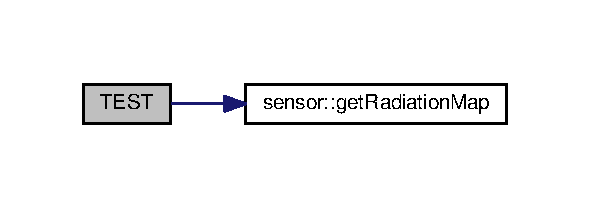
\includegraphics[width=283pt]{testSensor_8cpp_acde73c74a87cd4e2a6be903ae254b3ae_cgraph}
\end{center}
\end{figure}



%--- End generated contents ---

% Index
\backmatter
\newpage
\phantomsection
\clearemptydoublepage
\addcontentsline{toc}{chapter}{Index}
\printindex

\end{document}
